\documentclass[a4paper,11pt,oneside]{book}

% Essential packages
\usepackage[english]{babel}
\usepackage[utf8]{inputenc}
\usepackage[T1]{fontenc}
\usepackage{amsmath, amssymb, amsthm}  
\usepackage{graphicx}  
\usepackage{listings}                
\usepackage{xcolor}                  
\usepackage[most]{tcolorbox}                
\usepackage{enumitem}                   
\usepackage{float} 
\usepackage{titlesec}
\usepackage{algorithm}
\usepackage{algpseudocode}
\usepackage{pdfpages}
\usepackage{pgfplots}
\pgfplotsset{width=10cm,compat=1.15}


\usepackage[hidelinks,
            colorlinks=true,
            linkcolor=blue,
            urlcolor=blue,
            citecolor=blue,
            bookmarks=true,
            bookmarksopen=true,
            bookmarksnumbered=true,
            pdfstartview=FitH,
            pdftitle={Machine Learning Exams Collection},
            pdfauthor={Your Name},
            pdfsubject={Machine Learning},
            pdfkeywords={Machine Learning, Exams, Solutions},
            pdfencoding=auto,
            unicode=true
]{hyperref}


% Define colors for different elements
\definecolor{solutioncolor}{RGB}{240, 247, 255}
\definecolor{codebackground}{RGB}{248, 248, 248}
\definecolor{commentcolor}{RGB}{0, 128, 0}

\DeclareMathOperator*{\argmax}{arg\,max}
\DeclareMathOperator*{\argmin}{arg\,min}

% Custom styling for code listings
\lstset{
    backgroundcolor=\color{codebackground},
    commentstyle=\color{commentcolor},
    basicstyle=\ttfamily\small,
    breaklines=true,
    numbers=left,
    numberstyle=\tiny,
    frame=single,
    tabsize=2
}

% Custom environment for questions
\newcounter{question}[section]
\newenvironment{question}[1][]
    {\refstepcounter{question}\par\medskip
        \noindent\textbf{Question \thequestion.} \rmfamily #1\rmfamily}
    {\par\medskip}

    \newtcolorbox{solution}{
        enhanced,
        breakable,
        parbox=false,
        colback=white,
        colframe=black!70,
        arc=0mm,
        outer arc=0mm,
        leftrule=2pt,
        rightrule=0pt,
        toprule=0.5pt,
        bottomrule=0.5pt,
        left=4mm,
        right=4mm,
        top=2mm,
        bottom=2mm,
        title=\textbf{\sffamily Solution},
        fontupper=\normalfont
    }

\titleformat{\chapter}[display]
    {\normalfont\huge\bfseries}
    {Exam \thechapter} 
    {0pt}
    {\huge}

\titlespacing*{\chapter}
    {0pt} 
    {0pt}  
    {10pt}


\title{Machine Learning Exams Collection\\
University of Padua\\[1em]
\author{by \href{https://github.com/antoniooodev}{Antonio Tangaro}}
\date{Last update: \today}
\href{https://github.com/antoniooodev}{
\includegraphics[width=2cm]{images/github-mark.png}}}


\begin{document}

\maketitle
\tableofcontents

\chapter*{Introduction}
    \addcontentsline{toc}{chapter}{Introduction}
    This document is a collection of Machine Learning exam solutions from the course held between 2018 and 2022. The material is organized chronologically, with each chapter representing a different exam date.

    Each exam chapter follows a consistent structure:
    \begin{itemize}
        \item The chapter title indicates the exam date.
        \item The exam text is presented first, including any figures or tables.
        \item The solutions are provided in dedicated solution blocks using the \texttt{solution} environment.
        \item Mathematical formulas and equations are formatted using appropriate LaTeX notation.
        \item Figures and diagrams are included where necessary to support the explanations.
    \end{itemize}

    Each solution aims to provide clear explanations of concepts, mathematical derivations where required, and practical implementations when necessary. The document serves as both a reference for exam preparation and a comprehensive review of key machine learning concepts.

%-----------------------------------------------------------------------------------------------

\chapter{Quiz}

\section{Multiple Choice Questions}

\begin{enumerate}

    \item The goal of supervised learning is:
    \begin{enumerate}[label=\alph*)]
        \item to learn useful features
        \item None of the above
        \item to learn a neural network
        \item to learn a model with low generalization error
        \item to learn a model with low training error
    \end{enumerate}

    \item If you flip 10 times a coin that has probability 0.25 to give tail, the probability that you obtain 10 heads is:
    \begin{enumerate}[label=\alph*)]
        \item (1 - 0.25) $\times$ 10
        \item (1 - 0.25)$^{10}$
        \item None of the above
        \item (0.25)$^{10}$
        \item 0.25 $\times$ 10
    \end{enumerate}

    \item To use the ERM approach means that we learn a model by:
    \begin{enumerate}[label=\alph*)]
        \item finding the hypothesis with smallest training error
        \item finding the hypothesis with smallest generalization error
        \item finding the hypothesis that minimizes the expected regularization
        \item None of the above
        \item finding the hypothesis with smallest complexity
    \end{enumerate}

    \item The difference between classification and regression is given by:
    \begin{enumerate}[label=\alph*)]
        \item the loss function L you can use
        \item the label set Y
        \item None of the above
        \item the type of models you can use (e.g., SVM vs linear models)
        \item the approach used to find the model
    \end{enumerate}

    \clearpage
    \item What does "overfitting" refer to?
    \begin{enumerate}[label=\alph*)]
        \item Failing to converge during training
        \item None of the above
        \item Learning a model that performs well on training data but poorly on new data
        \item Learning a model that is too simple
        \item Learning a model that has perfect accuracy on all datasets
    \end{enumerate}

    \item For an hypothesis class H, being PAC learnable with respect to a loss function L, means:
    \begin{enumerate}[label=\alph*)]
        \item that for some D we can find the best h in H, independently of the amount of data
        \item that for some D we can find the best h in H, with enough data
        \item None of the above
        \item that for all D we can find the best h in H, independently of the amount of data
        \item that for all D we can find the best h in H, with enough data
    \end{enumerate}

    \item What is the main idea behind the concept of bias-complexity trade-off?
    \begin{enumerate}[label=\alph*)]
        \item Balancing the trade-off between model simplicity and interpretability
        \item Balancing the trade-off between accuracy and training time
        \item Balancing the trade-off between estimation error and approximation error
        \item Balancing the trade-off between feature selection and feature engineering
        \item None of the above
    \end{enumerate}

    \item What is the purpose of regularization?
    \begin{enumerate}[label=\alph*)]
        \item To increase model complexity so to prevent overfitting
        \item None of the above
        \item To reduce model complexity so to prevent overfitting
        \item To eliminate bias in the model
        \item To improve training speed
    \end{enumerate}

    \clearpage
    \item What is the purpose of validation?
    \begin{enumerate}[label=\alph*)]
        \item To assess the model's performance on the training set
        \item To train the model on multiple datasets
        \item None of the above
        \item To obtain a good estimate of the generalization error
        \item To compare different models on unseen data
    \end{enumerate}

    \item What is a main difference between SVMs and linear models?
    \begin{enumerate}[label=\alph*)]
        \item None of the above
        \item SVM can be used to learn models that are polynomial in the features
        \item there is no difference
        \item SVMs can be used only for linearly separable data
        \item SVMs consider the margin of the model, linear models do not
    \end{enumerate}

    \item The VC dimension is a measure of:
    \begin{enumerate}[label=\alph*)]
        \item None of the above
        \item the dimension of each point in a dataset
        \item the complexity of an hypothesis class
        \item the number of features in a model
        \item the generalizability of an hypothesis
    \end{enumerate}

    \item What is the primary goal of clustering?
    \begin{enumerate}[label=\alph*)]
        \item assigning labels to data points
        \item None of the above
        \item identifying patterns in unlabeled data
        \item predicting a continuous target variable
        \item classifying data into predefined categories
    \end{enumerate}

    \item Let $X, Y, D, \ell(x, y), \mathcal{H}, h, S$ defined as usual during the course. The definition of training error $L_S(h)$ is:
    \begin{enumerate}[label=\alph*)]
        \item $L_S(h) = E_{x,y \sim D}[\ell(h(x) - y)^2]$
        \item $L_S(h) = \frac{1}{|S|} \sum_{(x_i, y_i) \in S} (h(x_i) - y_i)^2$
        \item $L_S(h) = E_{x,y \sim D}[\ell(h(x), y)]$
        \item $L_S(h) = \frac{1}{|S|} \sum_{(x_i, y_i) \in S} \ell(h(x_i), y_i)$
        \item none of the above
    \end{enumerate}

    \item Let $X, Y, D, \ell(x, y), \mathcal{H}, h, S$ defined as usual during the course. The definition of generalization error $L_D(h)$ is:
    \begin{enumerate}[label=\alph*)]
        \item $L_D(h) = E_{x,y \sim D}[\ell(h(x) - y)^2]$
        \item $L_D(h) = \frac{1}{|S|} \sum_{(x_i, y_i) \in S} (h(x_i) - y_i)^2$
        \item $L_D(h) = E_{x,y \sim D}[\ell(h(x), y)]$
        \item $L_D(h) = \frac{1}{|S|} \sum_{(x_i, y_i) \in S} \ell(h(x_i), y_i)$
        \item none of the above
    \end{enumerate}

    \item The realizability assumption is defined as:
    \begin{enumerate}[label=\alph*)]
        \item there exists $h^* \in \mathcal{H}$ with $L_S(h) = 0$
        \item there exists $h^* \in \mathcal{H}$ with $L_D(h) = 0$
        \item ERM finds $h^* \in \mathcal{H}$ such that $L_S(h) = 0$
        \item ERM finds $h^* \in \mathcal{H}$ such that $L_D(h) = 0$
        \item none of the above
    \end{enumerate}

\end{enumerate}

\clearpage
\section{Answer Key}

\begin{enumerate}
    \item (1, d)
    \item (2, b)
    \item (3, a)
    \item (4, b)
    \item (5, c)
    \item (6, c)
    \item (7, c)
    \item (8, c)
    \item (9, e)
    \item (10, e)
    \item (11, c)
    \item (12, c)
    \item (13, d)
    \item (14, c)
    \item (15, b)
\end{enumerate}


%-----------------------------------------------------------------------------------------------

\chapter{31 January 2023}

\begin{figure}[H]
    \centering
    \begin{minipage}{0.45\textwidth}
        \includegraphics[width=\textwidth,page=3]{images/ex1_31_Jan_2023.png}
    \end{minipage}
    \hfill
    \begin{minipage}{0.45\textwidth}
        \includegraphics[width=\textwidth,page=5]{images/ex2_31_Jan_2023.png}
    \end{minipage}
    
    \vspace{1cm}
    
    \centering
    \begin{minipage}{0.45\textwidth}
        \includegraphics[width=\textwidth,page=7]{images/ex3_31_Jan_2023.png}
    \end{minipage}
    \hfill
    \begin{minipage}{0.45\textwidth}
        \includegraphics[width=\textwidth,page=9]{images/ex4_31_Jan_2023.png}
    \end{minipage}
\end{figure}
\clearpage

\section{Exercise 1}
    Consider the problem of supervised learning.
    \begin{enumerate}
        \item Describe all the components of the formal statistical learning model (domain set, ...) and the general goal of supervised learning.
            \begin{solution}
                A supervised learning problem consists of the following elements:
                \begin{itemize}
                    \item \textbf{Input space} $X$: The set of possible input instances.
                    \item \textbf{Output space} $Y$: The set of possible labels (discrete for classification, continuous for regression).
                    \item \textbf{Probability distribution} $D$: The unknown distribution over $X \times Y$ that generates data.
                    \item \textbf{Hypothesis class} $\mathcal{H}$: A set of functions $h : X \to Y$ representing possible models.
                    \item \textbf{Loss function} $\ell(h(x), y)$: A function that quantifies the error of a hypothesis on an individual example.
                    \item \textbf{Expected risk} $L_D(h)$: The average loss over the true distribution:
                    \[
                    L_D(h) = \mathbb{E}_{(x,y) \sim D} [\ell(h(x), y)].
                    \]
                    \item \textbf{Empirical risk} $L_S(h)$: The average loss over a training sample $S = \{(x_i, y_i)\}_{i=1}^{m}$:
                    \[
                    L_S(h) = \frac{1}{m} \sum_{i=1}^{m} \ell(h(x_i), y_i).
                    \]
                \end{itemize}
                The goal of supervised learning is to find a hypothesis $h \in \mathcal{H}$ that minimizes the expected risk $L_D(h)$. Since $D$ is unknown, we use empirical risk minimization (ERM) to approximate it.
            \end{solution}
        
        \clearpage
        \item Formally define when a training set is $\epsilon$-representative.
            \begin{solution}
                A training set $S$ is $\varepsilon$-\textbf{representative} for a hypothesis class $\mathcal{H}$ if the empirical risk is a good approximation of the expected risk for all hypotheses:
                \[
                \sup_{h \in \mathcal{H}} |L_S(h) - L_D(h)| \leq \varepsilon.
                \]
                This ensures that the empirical risk does not deviate from the expected risk by more than $\varepsilon$, making $S$ a reliable approximation of the true distribution.
            \end{solution}
            
        \item Provide and prove the upper bound to the generalization error $L_D(h_S)$ of the hypothesis $h_S$ picked by empirical risk minimization when the training set is $\frac{\epsilon}{2}$-representative (briefly motivating all the steps of the proof).
            \begin{solution}
                We prove that if $S$ is $\frac{\varepsilon}{2}$-representative, the generalization error of the empirical risk minimizer $h_S$ satisfies:
                \[
                L_D(h_S) \leq L_D(h^*) + \varepsilon,
                \]
                where $h^* = \arg\min_{h \in \mathcal{H}} L_D(h)$ is the optimal hypothesis.
                
                \textbf{Proof:}
                \begin{enumerate}
                    \item By assumption, $S$ is $\frac{\varepsilon}{2}$-representative, meaning:
                    \[
                    \sup_{h \in \mathcal{H}} |L_S(h) - L_D(h)| \leq \frac{\varepsilon}{2}.
                    \]
                    \item Since $h_S$ is chosen by ERM, it satisfies:
                    \[
                    L_S(h_S) \leq L_S(h^*).
                    \]
                    \item Applying the $\frac{\varepsilon}{2}$-representative property:
                    \[
                    L_D(h_S) \leq L_S(h_S) + \frac{\varepsilon}{2},
                    \]
                    \[
                    L_D(h^*) \leq L_S(h^*) + \frac{\varepsilon}{2}.
                    \]
                    \item Substituting $L_S(h_S) \leq L_S(h^*)$ into the first inequality:
                    \[
                    L_D(h_S) \leq L_S(h^*) + \frac{\varepsilon}{2}.
                    \]
                    \item Using $L_S(h^*) \leq L_D(h^*) + \frac{\varepsilon}{2}$, we obtain:
                    \[
                    L_D(h_S) \leq L_D(h^*) + \frac{\varepsilon}{2} + \frac{\varepsilon}{2} = L_D(h^*) + \varepsilon.
                    \]
                \end{enumerate}
                Thus, the generalization error of $h_S$ is at most $\varepsilon$ worse than the best possible hypothesis in $\mathcal{H}$.
            \end{solution}    
    \end{enumerate}

    \section{Exercise 2}
    \begin{enumerate}
        \item Describe the stochastic gradient descent (SGD) algorithm (in general).
            \begin{solution}
                Stochastic Gradient Descent (SGD) is an optimization algorithm designed to minimize an objective function, typically a loss function, by iteratively updating the model parameters using a single randomly chosen data point per iteration.
                
                The general update rule for SGD is:
                \[
                w^{(t+1)} = w^{(t)} - \eta \nabla_w \ell(w; x_i, y_i)
                \]
                where:
                \begin{itemize}
                    \item $w^{(t)}$ represents the model parameters at iteration $t$.
                    \item $\eta$ is the \textbf{learning rate}, which controls the step size of the update.
                    \item $\nabla_w \ell(w; x_i, y_i)$ is the \textbf{gradient} of the loss function with respect to the parameters, computed using only a single example $(x_i, y_i)$.
                \end{itemize}
                Unlike \textbf{Batch Gradient Descent (GD)}, which computes the gradient using the entire dataset at each iteration, SGD updates the model parameters using only \textbf{one sample at a time}, making it more efficient for large-scale problems.
            \end{solution}
        \clearpage
        \item What is the main advantage of SGD with respect to the gradient descent (GD) algorithm?
            \begin{solution}
                SGD has several advantages over Gradient Descent (GD):
                
                \begin{enumerate}
                    \item \textbf{Computational efficiency:}
                    \begin{itemize}
                        \item GD computes the gradient over the entire dataset, making it inefficient for large datasets.
                        \item SGD updates the parameters using only one sample per iteration, significantly reducing computational cost.
                    \end{itemize}
                
                    \item \textbf{Faster convergence for large datasets:}
                    \begin{itemize}
                        \item SGD performs more frequent updates, allowing faster convergence compared to GD in large-scale scenarios.
                        \item GD requires processing all samples before each update, slowing down the process.
                    \end{itemize}
                
                    \item \textbf{Better for non-convex optimization:}
                    \begin{itemize}
                        \item The randomness in SGD updates introduces noise, preventing the risk of getting stuck in poor-quality local minima.
                        \item GD, being deterministic, is more likely to converge to a local minimum rather than a global one.
                    \end{itemize}
                
                    \item \textbf{Online learning capability:}
                    \begin{itemize}
                        \item SGD is suitable for \textbf{online learning}, where data arrives sequentially and must be processed immediately.
                        \item GD requires the entire dataset to be available before starting training, making it less suitable for real-time applications.
                    \end{itemize}
                \end{enumerate}
                
                Consequently, \textbf{SGD is preferred for large datasets and online learning due to its computational efficiency and ability to escape poor local minima}.
            \end{solution}
            
        \item Consider a regression problem where the training data is $S = \{(x_i, y_i), (x_2, y_2), \dots, (x_m, y_m)\}$ with $x_i = [x_{i,1}, x_{i,2}] \in \mathbb{R}^2$ and $y_i \in \mathbb{R}$ for $i=1, \dots, m$.
            Assume the hypothesis class $\mathcal{H}$ is given by (simplified) linear models, that is, $\mathcal{H}$ is defined as $\mathcal{H} = \{h_w(x): h_w(x) = w_1x_1 + w_2x_2, w = [w_1, w_2] \in \mathbb{R}^2\}$, with $x = [x_1, x_2]$. Assume that the loss function is $\ell(h_w(x), y) = (h_w(x) - y)^2$, and that SGD is used to learn a model from the training data $S$.
            \\ Write the SGD update when the hypothesis class $\mathcal{H}$ is as described above.

                \begin{solution}
                    Consider a \textbf{linear regression problem} with a training dataset:
                    \[
                    S = \{(x_1, y_1), (x_2, y_2), \dots, (x_m, y_m)\}
                    \]
                    where:
                    \begin{itemize}
                        \item Each input $x_i$ is a two-dimensional vector $x_i = [x_{i,1}, x_{i,2}] \in \mathbb{R}^2$.
                        \item Each output $y_i$ is a real number $y_i \in \mathbb{R}$.
                    \end{itemize}
                    
                    The hypothesis class consists of linear models:
                    \[
                    h_w(x) = w_1 x_1 + w_2 x_2
                    \]
                    where the parameter vector is $w = [w_1, w_2] \in \mathbb{R}^2$.
                    
                    The loss function used is the \textbf{squared loss}:
                    \[
                    \ell(h_w(x), y) = (h_w(x) - y)^2.
                    \]
                    
                    To compute the SGD update, we first derive the gradient of the loss function with respect to $w$:
                    \[
                    \nabla_w \ell(h_w(x_i), y_i) = 2 (h_w(x_i) - y_i) \nabla_w h_w(x_i).
                    \]
                    
                    Since $h_w(x_i) = w_1 x_{i,1} + w_2 x_{i,2}$, the partial derivatives are:
                    \[
                    \frac{\partial h_w}{\partial w_1} = x_{i,1}, \quad \frac{\partial h_w}{\partial w_2} = x_{i,2}.
                    \]
                    
                    Thus, the gradient is:
                    \[
                    \nabla_w \ell(h_w(x_i), y_i) = 2 (h_w(x_i) - y_i) [x_{i,1}, x_{i,2}].
                    \]
                    
                    Applying the SGD update rule:
                    \[
                    w_j^{(t+1)} = w_j^{(t)} - \eta \frac{\partial \ell}{\partial w_j}, \quad \text{for } j = 1, 2.
                    \]
                    
                    Substituting the gradient:
                    \[
                    w_1^{(t+1)} = w_1^{(t)} - \eta \cdot 2 (h_w(x_i) - y_i) x_{i,1},
                    \]
                    \[
                    w_2^{(t+1)} = w_2^{(t)} - \eta \cdot 2 (h_w(x_i) - y_i) x_{i,2}.
                    \]
                    
                    Therefore, for each randomly selected training point $(x_i, y_i)$, the weight update follows:
                    \[
                    w^{(t+1)} = w^{(t)} - 2\eta (h_w(x_i) - y_i) x_i.
                    \]
                    
                    where $x_i$ is the feature vector $[x_{i,1}, x_{i,2}]$.
                \end{solution}  
    \end{enumerate}


\clearpage
\section{Exercise 3}
    Consider neural networks (NNs) for classification with 0-1 loss.
    \begin{enumerate}
        \item Describe what you need to fix to define the hypothesis class of a NN, and what is instead learned from data.
        
            \begin{solution}
                To define the \textbf{hypothesis class} of a neural network, we must fix:
                \begin{itemize}
                    \item The number of \textbf{hidden layers} and \textbf{neurons per layer}.
                    \item The \textbf{activation function} for each layer, in this case, the \textbf{sign function}.
                    \item The \textbf{weight constraints}, here limited to $\{-1, 0, 1\}$.
                    \item The \textbf{connectivity structure}, which defines how neurons are linked.
                \end{itemize}
                
                Instead, what is \textbf{learned from data} during training includes:
                \begin{itemize}
                    \item The \textbf{weights} connecting neurons.
                    \item The \textbf{bias terms}, which allow neurons to shift activation thresholds.
                    \item A function that approximates the \textbf{decision boundary} by minimizing a loss function.
                \end{itemize}
                
                Once these elements are set, the neural network learns an optimal function by adjusting its weights through optimization algorithms.
            \end{solution}
        
        \clearpage
        \item Let $x = [x_1, x_2]$, with $x_1, x_2 \in \{-1, 1\}$. Consider the NN in the figure below, where the activation function for each hidden node and the output node is the $sign$ function. Assume that the weights are constrained to be in the set $\{-1, 0, 1\}$. You want your network to represent the function $f$ that is 1 when the input is $[1, 1]$ or $[-1, -1]$ (for all other inputs the function is -1).
        \begin{enumerate}
            \item Find the network's weights so that the network represents the function $f$ described above. Write the weights in the dashed boxes in the figure.
            \item Briefly describe the procedure you used to find the weights.
        \end{enumerate}

        \begin{figure}[H]
            \centering
            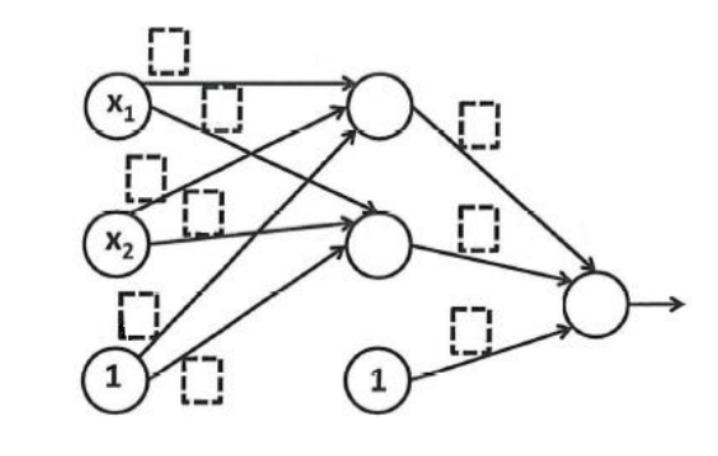
\includegraphics[width=0.4\textwidth,height=0.6\textheight,keepaspectratio]{images/3_31_Jan_2023.png}
        \end{figure}

            \begin{solution}
                The goal is to design a neural network that implements the function:
                \[
                f(x_1, x_2) = 1 \quad \text{if} \quad (x_1, x_2) = (1,1) \text{ or } (-1,-1), \quad \text{else} \quad f(x) = -1.
                \]
                Since the activation function is the \textbf{sign function}, we need to construct a \textbf{two-layer network} that correctly classifies these inputs.
                
                \subsection*{(a) Choosing the Weights}
                The required weights are assigned as follows:
                \begin{itemize}
                    \item \textbf{Hidden Layer Weights:}
                    \begin{itemize}
                        \item One neuron detects when $x_1 = x_2$ by computing $x_1 + x_2$.
                        \item Another neuron detects when $x_1 \neq x_2$ using $x_1 - x_2$.
                    \end{itemize}
                    \item \textbf{Output Layer Weights:}
                    \begin{itemize}
                        \item The output neuron applies the \textbf{sign function} to distinguish the correct class.
                    \end{itemize}
                \end{itemize}

                \begin{figure}[H]
                    \centering
                    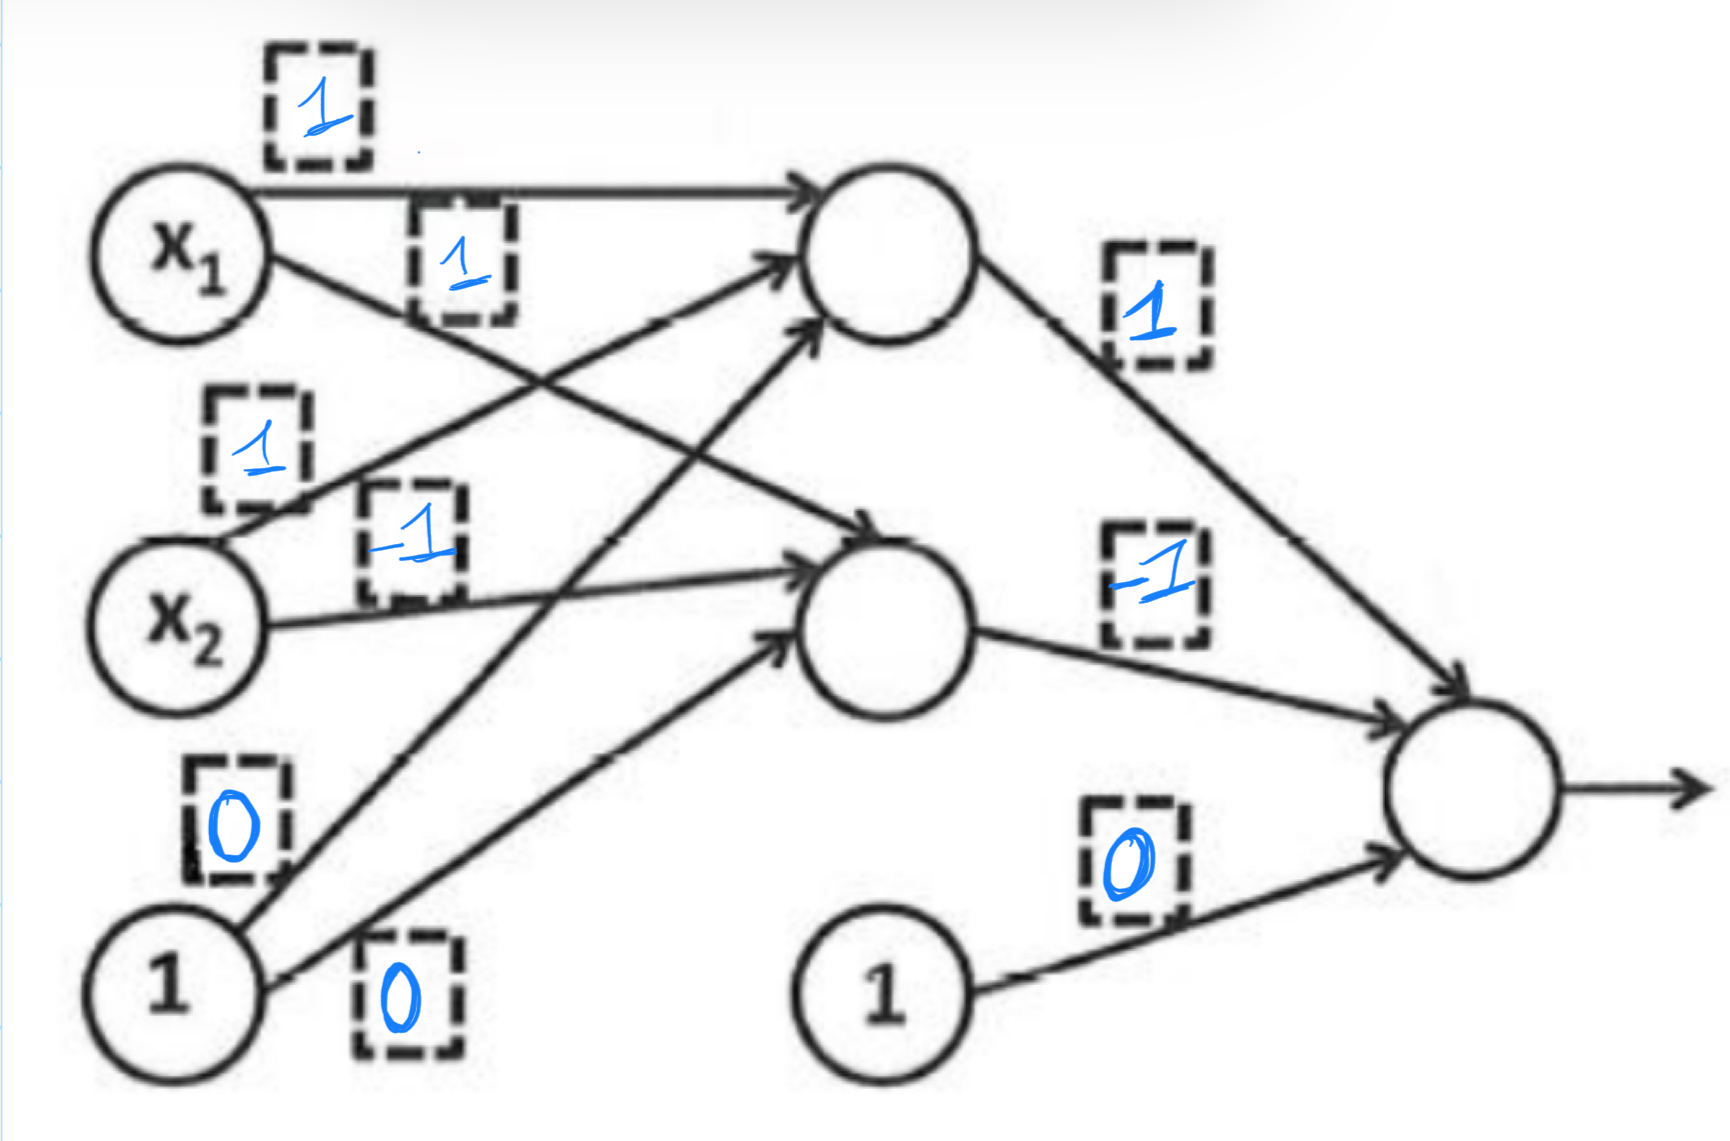
\includegraphics[width=0.9\textwidth,height=0.9\textheight,keepaspectratio]{images/2_4_31_Jan_2023.jpeg}
                \end{figure}
                
                This weight assignment ensures that:
                \begin{itemize}
                    \item When $x_1 = x_2$, the first hidden neuron is active.
                    \item When $x_1 \neq x_2$, the second hidden neuron is active.
                    \item The output neuron sums these signals and applies the \textbf{sign function}, correctly classifying the input.
                \end{itemize}
                
                \subsection*{(b) Procedure for Finding the Weights}
                The method follows a logical breakdown:
                \begin{enumerate}
                    \item \textbf{Analyze the function}: The network must recognize cases where $x_1 = x_2$.
                    \item \textbf{Design the hidden neurons}: One neuron detects equality, another detects inequality.
                    \item \textbf{Assign weights}: Set values to enforce correct neuron activation.
                    \item \textbf{Validate output behavior}: Ensure the final neuron applies the correct decision boundary.
                \end{enumerate}
                
                This systematic approach guarantees correct classification while respecting the constraints on weights.
            \end{solution}  
    \end{enumerate}

\clearpage
\section{Exercise 4}
    Consider the clustering problem.
    \begin{enumerate}
        \item Briefly describe linkage-based clustering: what is the input, what is the output, the general algorithm it employs, and a termination condition.
            \begin{solution}
                \textbf{Linkage-based clustering} is a hierarchical clustering method used to partition a dataset into clusters based on a \textbf{distance function}. 
                
                \textbf{Input:} 
                \begin{itemize}
                    \item A set $X$ of objects.
                    \item A \textbf{distance function} $d: X \times X \to \mathbb{R}^+$, which must satisfy properties like symmetry, identity of indiscernibles, and the triangle inequality.
                \end{itemize}
                
                \textbf{Output:} 
                A \textbf{dendrogram}, representing how clusters merge at different distance thresholds.
                
                \textbf{Algorithm:}
                \begin{enumerate}
                    \item \textbf{Initialization:} Each data point starts as its own cluster.
                    \item \textbf{Iterative Merging:} The two closest clusters are merged at each step based on a chosen \textbf{linkage criterion}.
                    \item \textbf{Termination Condition:} The process stops when a predefined stopping criterion is met.
                \end{enumerate}
                
                \textbf{Common termination conditions:}
                \begin{itemize}
                    \item \textbf{Fixed number of clusters:} The process stops when $k$ clusters remain.
                    \item \textbf{Distance threshold:} Clusters are not merged if the minimum distance between them exceeds a threshold $r$.
                    \item \textbf{Complete merging:} The process continues until all points belong to a single cluster, producing a dendrogram.
                \end{itemize}
            \end{solution}
        \clearpage
        \item Consider single linkage clustering. Describe how it is obtained by the general linkage-based clustering (no pseudocode needed).
            \begin{solution}
                \textbf{Single linkage clustering} is a specific type of linkage-based clustering where the distance between two clusters $A$ and $B$ is defined as:
                \[
                D(A, B) = \min \{ d(x, x') \mid x \in A, x' \in B \}.
                \]
                This means that at each step, the algorithm merges the two clusters whose \textbf{closest points} have the smallest distance.
                
                \textbf{Characteristics:}
                \begin{itemize}
                    \item \textbf{Chaining effect:} The algorithm tends to create elongated clusters rather than compact ones.
                    \item \textbf{Hierarchical approach:} The process follows the general linkage-based clustering structure but differs in how it measures distances between clusters.
                \end{itemize}
                
                At each iteration, the algorithm identifies and merges the two clusters with the smallest minimum inter-cluster distance. This process continues until a stopping condition is met.
            \end{solution}
        
        \clearpage
        \item Show the output of single linkage clustering when the input is given by the points in $\mathbb{R}^2$ shown as crosses below and the termination condition is given by having the points partitioned in $k=2$ clusters. (You can draw directly in the figure below.) Briefly describe how the algorithm reaches such output.
            \begin{solution}
                The dataset consists of points in $\mathbb{R}^2$ arranged in a curved pattern. The task is to apply \textbf{single linkage clustering} and stop when \textbf{two clusters remain} ($k = 2$).
                
                \textbf{Algorithm Execution:}
                \begin{itemize}
                    \item Each point starts as its own cluster.
                    \item The algorithm finds and merges the two closest clusters at each iteration.
                    \item Due to the \textbf{chaining effect}, clusters gradually extend along the data distribution.
                    \item The process stops when only \textbf{two clusters remain}.
                \end{itemize}
                
                \textbf{Final Clustering Output:}
                The final partition consists of \textbf{two clusters}, corresponding to the \textbf{upper and lower sets of points} in the figure. These clusters reflect the chaining effect of single linkage, where points progressively merge based on their closest neighbor.
            \end{solution}
            
        \begin{figure}[H]
            \centering
            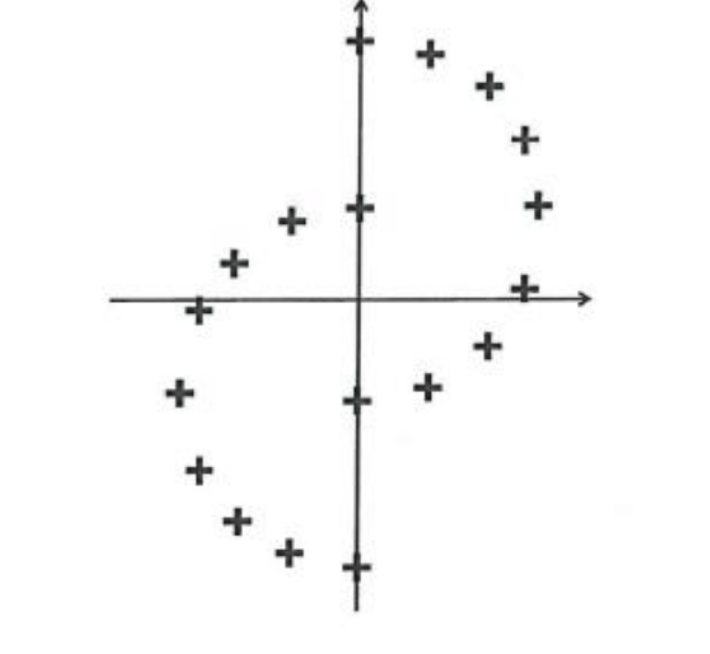
\includegraphics[width=0.4\textwidth,height=0.6\textheight,keepaspectratio]{images/4_31_Jan_2023.png}
        \end{figure}
    
    \end{enumerate}



%-----------------------------------------------------------------------------------------------

\chapter{16 February 2022}

\begin{figure}[H]
    \centering
    \begin{minipage}{0.45\textwidth}
        \includegraphics[width=\textwidth,page=3]{images/ex1_16_Feb_2022.png}
    \end{minipage}
    \hfill
    \begin{minipage}{0.45\textwidth}
        \includegraphics[width=\textwidth,page=5]{images/ex2_16_Feb_2022.png}
    \end{minipage}
    
    \vspace{1cm}
    
    \centering
    \begin{minipage}{0.45\textwidth}
        \includegraphics[width=\textwidth,page=7]{images/ex3_16_Feb_2022.png}
    \end{minipage}
    \hfill
    \begin{minipage}{0.45\textwidth}
        \includegraphics[width=\textwidth,page=9]{images/ex4_16_Feb_2022.png}
    \end{minipage}
\end{figure}
\clearpage

\section{Exercise 1}
    Consider the task of binary classification with 0-1 loss, domain set $\mathcal{X} = \mathbb{R}^d$, and hypothesis class $\mathcal{H} = \{h_w(x): h_w(x) = sign(<w,x>)\}$.
    \begin{enumerate}
        \item Clearly describe the perceptron algorithm, and provide a brief intuition for its update rule.
        \item With respect to the context above, what is is a tight value $\ell$ such $VCdim(\mathcal{H}) \geq \ell$? Prove that $VCdim(\mathcal{H}) \geq \ell$ (for your choice of $\ell$).
    \end{enumerate}

\section{Exercise 2}
    \begin{enumerate}
        \item Describe the stochastic gradient descent (SGD) algorithm (in general). What is the main advantage of SGD with respect to the gradient descent algorithm?
        \item Consider the regression problem with training data $S = \{(x_i, y_i), (x_2, y_2), \dots, (x_m, y_m)\}$ with $x_i = [x_{i,1}, x_{i,2}] \in \mathbb{R}^2$ and $y_i \in \mathbb{R}$ for $i=1, \dots, m$.
            Assume the hypothesis class $\mathcal{H}$ is given by the simple neural network with the architecture below, where the edge weights are $w_1$ and $w_2$.

            \begin{figure}[H]
                \centering
                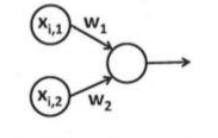
\includegraphics[width=0.4\textwidth,height=0.6\textheight,keepaspectratio]{images/2_16_Feb_2022.png}
            \end{figure}

            Assume the activation function for the output node is $\sigma(z) = z$ (the final prediction is the output of the output node), and the loss function is $\ell(h(x), y) = (h(x) - y)^2$.
            Write the SGD update when the hypothesis class $\mathcal{H}$ is as specified above.
    \end{enumerate}

\section{Exercise 3}
    Consider a regression problem with squared loss.
    \begin{enumerate}
        \item Formally define the label set $Y$, the loss function, the training error, and the generalization error.
        \item Consider the setting above with the addition of Tikhonov regularization. Describe the framework of regularized loss minimization (with Tikhonov regularization) and the relation of the parameter $\lambda$ with the decomposition of the generalization error in approximation error and estimation error.
        \item Assume the hypothesis class is given by linear models and Tikhonov regularization is used. Derive the formula for the best model in this case.
    \end{enumerate}

\section{Exercise 4}
    Consider a clustering problem
    \begin{enumerate}
        \item Briefly describe linkage-based clustering (what is the input, what is the output, the general algorithm it employs, and a termination condition).
        \item Consider single linkage clustering. Describe how it is obtained by the general linkage-based clustering (no pseudocode needed).
        \item Show the output of single linkage clustering when the input is given by the points in $\mathbb{R}^2$ as shown in the figure below and the termination condition is given by having the points partitioned in $k=2$ clusters. (You can draw directly in the figure below.) Briefly describe how the algorithm reaches such output.
            \begin{figure}[H]
                \centering
                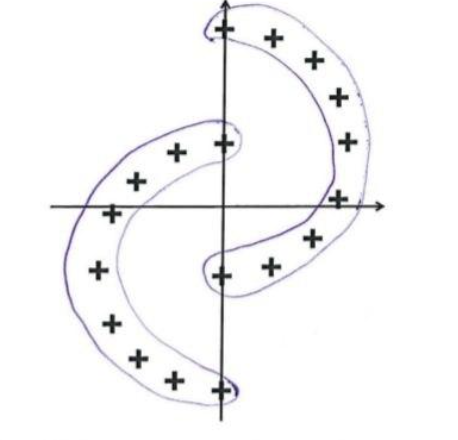
\includegraphics[width=0.4\textwidth,height=0.6\textheight,keepaspectratio]{images/4_16_Feb_2022.png}
            \end{figure}
    \end{enumerate}



%-----------------------------------------------------------------------------------------------

\chapter{1 February 2022}

\begin{figure}[H]
    \centering
    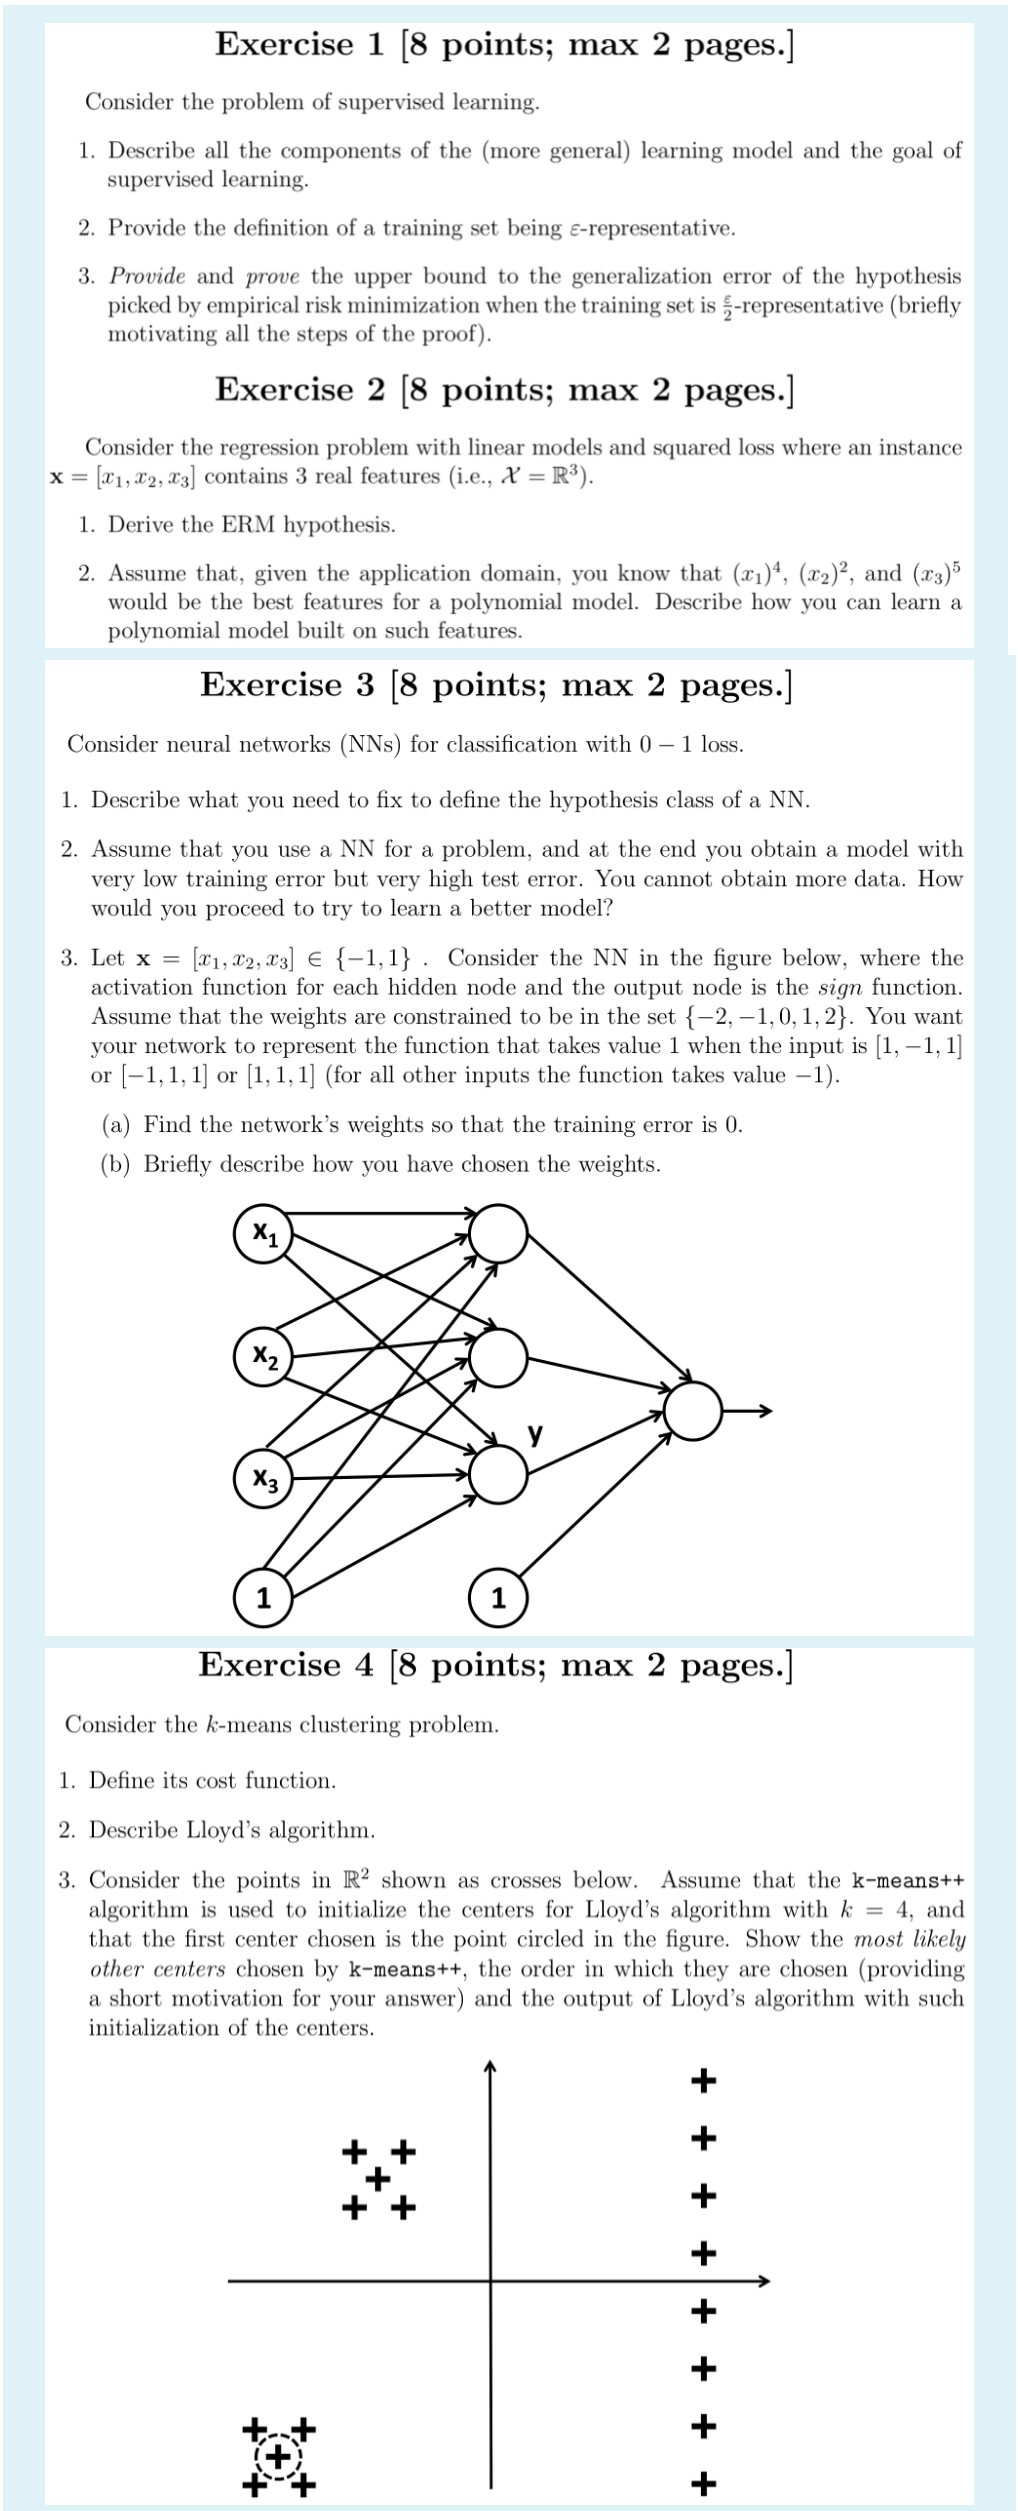
\includegraphics[width=0.8\textwidth,height=0.8\textheight,keepaspectratio]{images/1_Feb_22.png}
\end{figure}
\clearpage

\section{Exercise 1}
    Consider the problem of supervised learning.
    \begin{enumerate}
        \item Describe all the components of the (more general) learning model and the goal of supervised learning.
        \begin{solution}
            In supervised learning we have:
            \begin{itemize}
            \item An instance set $X$
            \item Label set $Y$
            \item Given a set $S = \{(\vec{x}_1, y_1),...,(\vec{x}_m, y_m)\}$ of $m$ labeled samples
            \end{itemize}
            
            Our goal is we have to choose an hypothesis class $H$ of functions $h: X \to Y$ and a loss function $l: H\times Z \to \mathbb{R}^+$, where $Z = X\times Y$, that tells us how much we lose by predicting $h(x)$ instead of the correct label $y_i$.
            
            The goal is to find an hypothesis $h \in H$ of low generalization error $L_D(h) = E_{z\sim D}[l(h,z)]$ where $z = (x,y)$ is sampled by an unknown distrib. $D$.
        \end{solution}
        \item Provide the definition of a training set being $\epsilon$-representative.
        \begin{solution}
            $S$ is $\varepsilon$-repr. if $\forall h \in H : |L_D(h)-L_S(h)| \leq \varepsilon$
        \end{solution}      
        \item Provide and prove the upper bound to the generalization error of the hypothesis picked by empirical risk minimization when the training set is $\frac{\epsilon}{2}$-representative (briefly motivating all the steps of the proof).
        \begin{solution}
            If $S$ is $\varepsilon/2$-repr. then $L_D(h_S) \leq \min_{h\in H} L_D(h) + \varepsilon$

            Proof:
            \begin{align*}
            \forall h \in H \quad L_D(h_S) &\leq L_S(h_S) + \varepsilon/2 \quad \text{[$\varepsilon/2$-repr.]} \\
            &\leq L_S(h) + \varepsilon/2 \quad \text{[ERM $(L_S(h_S) \leq L_S(h))$]} \\
            &\leq L_D(h) + \varepsilon/2 + \varepsilon/2 \quad \text{[$\varepsilon/2$-repr.]} \\
            &\leq L_D(h) + \varepsilon
            \end{align*}

            This is also true for $\argmin_{h\in H} L_D(h)$

            So $L_D(h_S) \leq \min_{h\in H} L_D(h) + \varepsilon$
        \end{solution}      
    \end{enumerate}

\section{Exercise 2}
    Consider the regression problem with linear models and squared loss where an instance
    $\mathbf{x} = [x_1, x_2, x_3]$ contains 3 real features (i.e., $\mathbf{X} = \mathbb{R}^3$).
    \begin{enumerate}
        \item Derive the ERM hypothesis.
        \begin{solution}
            $l(h, (x_i,y_i)) = (y_i - h(x_i))^2 = (y_i - \langle \vec{w}, \vec{x}_i \rangle)^2$
            
            $L_S(h) = \frac{1}{m} \sum_{i=1}^m (y_i - \langle \vec{w}, \vec{x}_i \rangle)^2 = (y_i - X\vec{w})^T(y_i - X\vec{w})$
            
            We have to minimize $L_S(h)$
            
            We can do it by picking the derivative = 0:
            
            \begin{align*}
            \frac{\partial L_S(h)}{\partial \vec{w}} &= 0 \Leftrightarrow -X^T(y_i - X\vec{w}) - X^T(y_i - X\vec{w}) = 0 \\
            &\Leftrightarrow -2X^T(y_i - X\vec{w}) = 0 \\
            &\Leftrightarrow X^Ty_i - X^TX\vec{w} = 0 \\
            &\Leftrightarrow \vec{w} = (X^TX)^{-1}X^Ty_i \quad \text{[it's invertible]}
            \end{align*}
        \end{solution}
        \item Assume that, given the application domain, you know that $(x_1)^2$, $(x_2)^2$, and $(x_3)^2$ would be the best features for a polynomial model. Describe how you can learn a polynomial model built on such features.
        \begin{solution}
            We can use feature expansion: we apply a transformation to each instance of the dataset: $x = [1, x_1, ..., x_1^2, ..., x_2, ..., x_3, ..., x_n]$. Then learn a linear model on this transformed dataset.
        \end{solution}
    \end{enumerate}

\clearpage
\section{Exercise 3}
    Consider neural networks (NNs) for classification with 0 - 1 loss.
    \begin{enumerate}
        \item Describe what you need to fix to define the hypothesis class of a NN.
        \begin{solution}
            We need to define:
            \begin{itemize}
            \item The number of hidden layers
            \item How many neurons we have in each layer
            \item The activation function we want to use: $\sigma = \{\text{sigmoid}, \tanh, ...\}$
            \end{itemize}
            
            The NN hypothesis class is $H_{(V,E,\sigma)}$
        \end{solution}
        \item Assume that you use a NN for a problem, and at the end you obtain a model with very low training error but very high test error. You cannot obtain more data. How would you proceed to try to learn a better model?
        \begin{solution}
            Low training error and high test error means we are overfitting.

            We can use several approaches:
            \begin{itemize}
            \item Probably the model is too complex so we can reduce the number of layers or number of neurons.

            \item We can use regularization that adds to the loss a term $\lambda\|\vec{w}\|^2$ that takes into account the model complexity and controls it with hyper parameter $\lambda$

            \item We can use dropout that at each iteration of the SGD ignores some neurons.

            \item Since we have a small amount of data, we can use cross-fold validation that allows us to train on several sub-sets of $S$ and test with 1 fold.
            \end{itemize}
        \end{solution}
        \clearpage
        \item Let $x = [x_1, x_2, x_3] \in {-1, 1}$. Consider the NN in the figure below, where the activation function for each hidden node and the output node is the sign function. Assume that the weights are constrained to be in the set ${-2, -1, 0, 1, 2}$. You want your network to represent the function that takes value 1 when the input is $[1, -1, 1]$ or $[-1, 1, 1]$ or $[1, 1, 1]$ (for all other inputs the function takes value -1).
        \begin{enumerate}
            \item Find the network's weights so that the training error is 0.
            \item Briefly describe how you have chosen the weights.
        \end{enumerate}
        \begin{figure}[H]
            \centering
            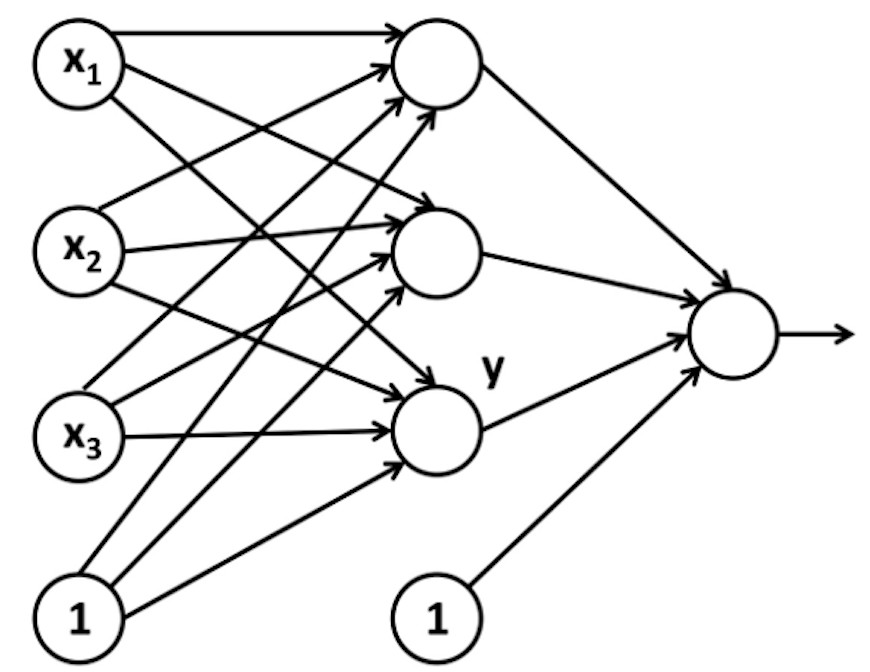
\includegraphics[width=0.4\textwidth,height=0.6\textheight,keepaspectratio]{images/graph_3_1_Feb_2022.png}
        \end{figure}
        \begin{solution}
            In class we have seen that a function $f:\{-1,1\}^d \to \{-1,1\}$ can be implemented by the network in the figure.
            
            \begin{itemize}
            \item The weights between the last 2 layers are all 1 except for the bias that is $1-k = -2$
            
            \item Each neuron in the hidden layer implements a function:
            $$y_i = sgn(\langle w,x \rangle)$$
            For each input that has as output 1 for a total of $k=3$ hidden neurons.
            Where its weights are the value of such instance except for the bias that is equal to: $d-1 = 2$
    
            \end{itemize}
            \begin{figure}[H]
                \centering
                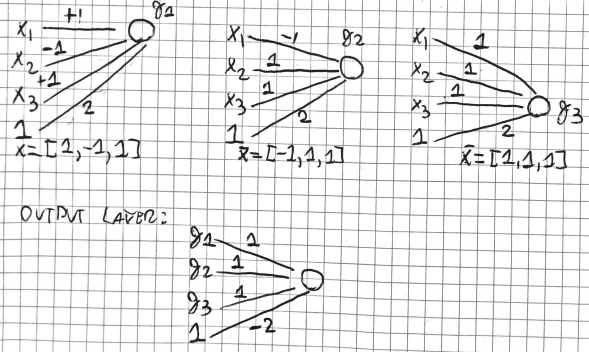
\includegraphics[width=0.6\textwidth,height=0.6\textheight,keepaspectratio]{images/graph_3_3_Feb_2022.png}
            \end{figure}
            \end{solution}
    \end{enumerate}

\section{Exercise 4}
    Consider the k-means clustering problem.
    \begin{enumerate}
        \item Define its cost function.
        \begin{solution}
            k-means cost function:
            $$\sum_{i=1}^k \sum_{x \in C_i} d(x, \mu_i)^2$$
            where $\mu_i$ with $i \in [1,...,k]$ are centroids
            \end{solution}
        \item Describe Lloyd's algorithm.
        \begin{solution}
            Lloyd algo.: $O(tkdm)$ time complexity\\
            where $k = \text{num. clusters}$, $m = \text{num. samples}$\\
            $d = \text{space dimension}$, $t = \text{num. iterations}$
            
            Input: $X = (x_1,...,x_m)$ with $x_i \in \mathbb{R}^d$, $k \in \mathbb{N}^+$\\
            Output: $\{\vec{\mu}_1,...,\vec{\mu}_k\}$ centroids, $C = \{C_1,...,C_k\}$ clustering of X
            
            \begin{algorithmic}[1]
            \State Initialize $\vec{\mu}_1^{(0)},...,\vec{\mu}_k^{(0)}$ at random \Comment{Assign instances}
            \State For $t = 0,...$ till convergence: \Comment{to the nearest cluster}
            \For{$i = 1,...,k$}
               \State $C_i \gets \{x \in X : i = \argmin_j d(x,\mu_j)\}$
            \EndFor
            \For{$i = 1,...,k$}
               \State $\vec{\mu}_i^{(t+1)} \gets \frac{1}{|C_i|}\sum_{x \in C_i} x$ \Comment{Update centroids}
            \EndFor
            \If{convergence reached}
               \State Return $\vec{\mu}_1^{(t+1)},...,\vec{\mu}_k^{(t+1)}$ and $C = \{C_1,...,C_k\}$
            \EndIf
            \end{algorithmic}
            
            Common convergence conditions:
            \begin{itemize}
            \item $\sum_{i=1}^k d(\vec{\mu}_i^{(t)}, \vec{\mu}_i^{(t+1)}) \leq \varepsilon$
            \item $\max_{i \in [1,...,k]}\{d(\vec{\mu}_i^{(t)}, \vec{\mu}_i^{(t+1)})\} \leq \varepsilon$
            \item Cost function on current iteration is not lower than the previous iteration
            \end{itemize}
            \end{solution}
        \item Consider the points in $\mathbb{R}^2$ shown as crosses below. Assume that the $k-means++$ algorithm is used to initialize the centers for Lloyd's algorithm with k = 4, and that the first center chosen is the point circled in the figure. Show the most likely other centers chosen by $k-means++$  (providing a short motivation for your answer) and the output of Lloyd's algorithm with such initialization of the centers.
        \begin{figure}[H]
            \centering
            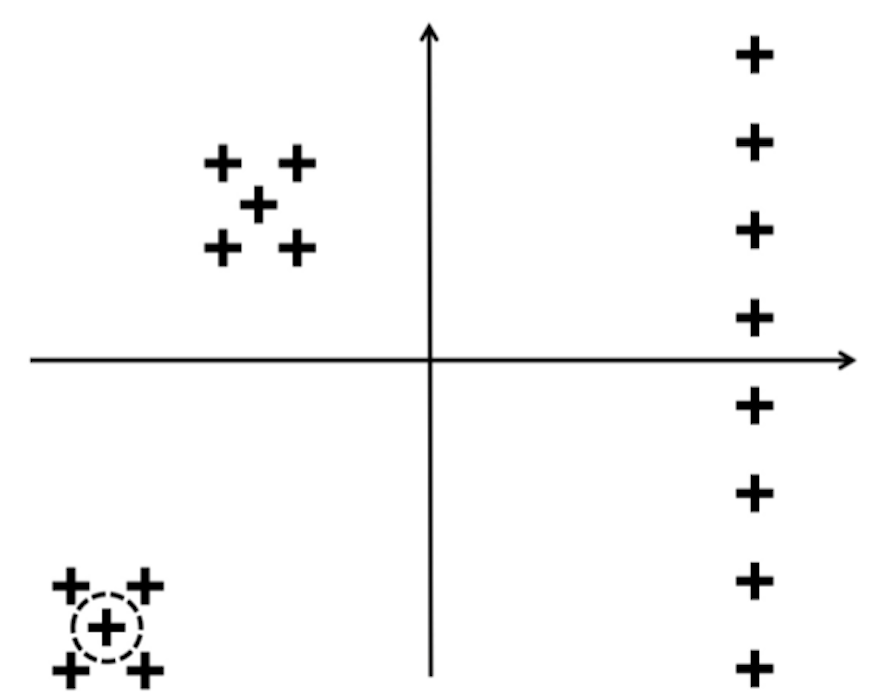
\includegraphics[width=0.5\textwidth,height=0.5\textheight,keepaspectratio]{images/graph_4_1_Feb_2022.png}
        \end{figure}
        \begin{solution}
            k-means++:
            
            \begin{algorithmic}[1]
            \State $\mu_1 \gets$ random $x \in X$
            \State $F = \{\mu_1\}$
            \For{$i = 2,...,k$}
               \State $\mu_i \gets \argmax_{x \in X \setminus F} d(x,F)^2$ \Comment{Distance from $x$ to each point in F}
               \State $F \gets F \cup \{\mu_i\}$
            \EndFor
            \State Return $F$
            \end{algorithmic}
            
            At each iteration picks the point that is farthest from the already chosen centroids (quadratic).
            
            So the order in which k-means++ chose the centroids is:
            
            \begin{figure}[H]
                \centering
                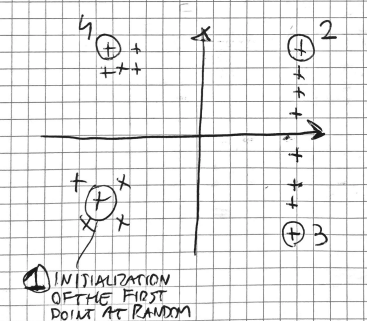
\includegraphics[width=0.4\textwidth,height=0.4\textheight,keepaspectratio]{images/graph_3_4_Feb_2022.png}
            \end{figure}
        \end{solution}
    \end{enumerate}

%-----------------------------------------------------------------------------------------------
\chapter{7 September 2021}

\begin{figure}[H]
    \centering
    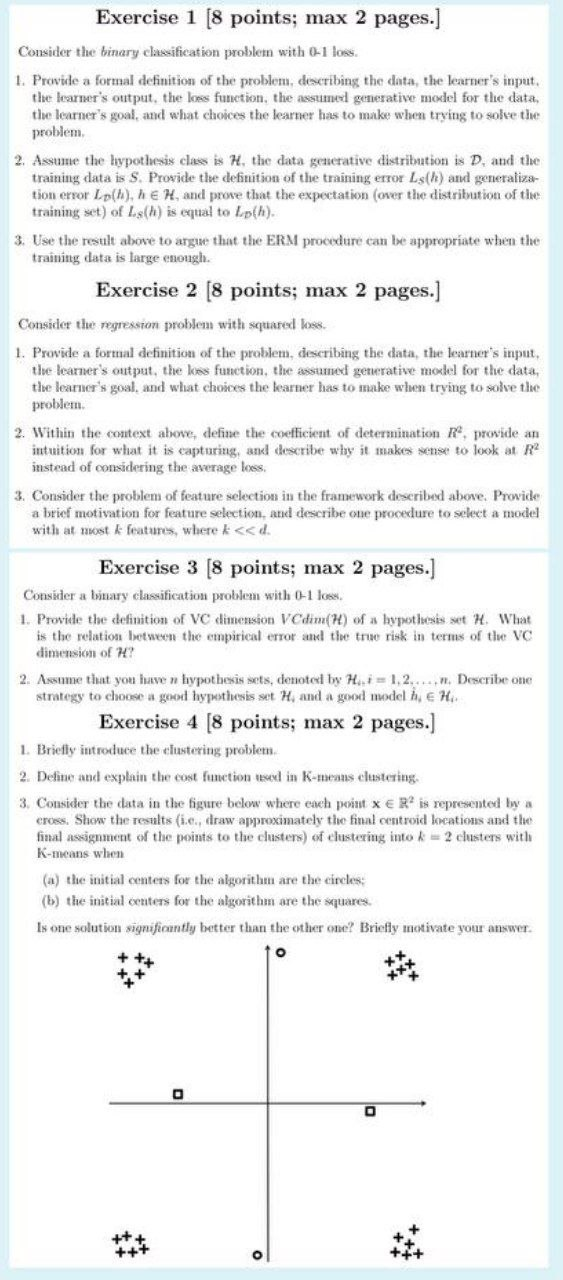
\includegraphics[width=0.8\textwidth,height=0.8\textheight,keepaspectratio]{images/7_Set_2021.jpg}
\end{figure}

\clearpage 
\section{Exercise 1}
Consider the binary classification problem with 0-1 loss.

\begin{enumerate}
\item Provide a formal definition of the problem, describing the data, the learner's input, the learner's output, the loss function, the assumed generative model for the data, the learner's goal, and what choices the learner has to make when trying to solve the problem.

\begin{solution}
    The binary classification problem with 0-1 loss is a supervised learning problem with:
    
    \begin{itemize}
    \item Domain set $X$ which is the set of all possible objects to make predictions about, where a domain point $\vec{x} \in X$ is called instance and is usually represented by a vector of features
    
    \item Label set $Y = \{-1, +1\}$, that defines the set of all possible labels in this case the labels are only 2
    \end{itemize}
    
    Given a training set $S = ((\mathbf{x}_1, y_1) ... (\mathbf{x}_m, y_m))$ with $x_i \in X, y_i \in Y$ $\forall i = 1,..,m$ we need to choose an hypothesis class H, which defines the possible models or classification rules, from which we can pick our model to make predictions, and a loss function $l: H \times Z \to \mathbb{R}^+$ where $Z = X \times Y$ that given an hypothesis provides a measure of how much we lose by predicting the value $h(\vec{x})$ for $\vec{x}$ instead of the correct value $y$. In particular in the case of 0-1 loss the function is exactly the following:
    
    $$l(h, (\vec{x},y)) = \begin{cases} 
    1 \text{ if } h(\vec{x}) \neq y \\
    0 \text{ if } h(\vec{x}) = y
    \end{cases}$$
    
    The goal is to find an hypothesis $\hat{h} \in H$ with low generalization error: $L_d(\hat{h}) = E_{z\sim D}[l(\hat{h},z)]$ where:
    
    \begin{itemize}
    \item $D$ is the unknown probability distribution over $Z$ from which $(x_i, y_i) \in S$ have been drawn (as independent samples).
    \end{itemize}
    \end{solution}

\clearpage 
\item Assume the hypothesis class is $\mathcal{H}$, the data generative distribution is $\mathcal{D}$, and the training data is $\mathcal{S}$. Provide the definition of the training error $L_S(h)$ and generalization error $L_{\mathcal{D}}(h)$, $h \in \mathcal{H}$, and prove that the expectation (over the distribution of the training set) of $L_S(h)$ is equal to $L_{\mathcal{D}}(h)$.

\begin{solution}
    Let:
    \begin{itemize}
    \item $X$ be the domain set, which is the set of all possible objects to make predictions about, where a domain point $\vec{x} \in X$ is called instance and is usually represented by a vector of features
    \item $Y$ be the label set that defines the set of all possible labels
    \item $S = ((\vec{x}_1, y_1) ... (\vec{x}_m, y_m))$ with $\vec{x}_i \in X, y_i \in Y$ $\forall i = 1,..,m$ be the training set
    \item $l: H\times Z \to \mathbb{R}^+$ where $Z = X\times Y$ be the loss function namely a function that given an hypothesis provides a measure of how much we lose by predicting the value $h(\vec{x})$ for $\vec{x}$ instead of the
    \item $D$ be the unknown distribution
    \item $H$ be the hypothesis class
    \end{itemize}
    
    We define the training error as: \\ $L_S(h) = \frac{1}{m}\sum_{i=1}^m l(h, (\vec{x}_i,y_i))$.
    
    We define the generalization error as: \\ $L_d(h) = E_{z\sim D}[l(h,z)]$ where $z = (\vec{x}, y)$

    \begin{align*}
    E[L_s(h)] &= E\left[\frac{1}{m}\sum_{i=1}^m l(h, (\vec{x}_i,y_i))\right] \\
    &= \frac{1}{m}\sum_{i=1}^m E[l(h, (\vec{x}_i,y_i))] \\
    &= \frac{1}{m}\sum_{i=1}^m L_d(h) \\
    &= L_d(h)
    \end{align*}
\end{solution}

\clearpage
\item Use the result above to argue that the ERM procedure can be appropriate when the training data is large enough.
\begin{solution}
    $L_s(h)$ is the probability that a pair $(\vec{x},y)$ taken uniformly at random from $S$ the event $h(\vec{x}) \neq y$. That means, if we compute $E[L_s(h)]$, then it is equal to $L_d(h)$ if we have enough data because $S$ is taken from $D$. Therefore $L_s(h) \approx L_d(h)$ because with enough data $E[L_s(h)] = L_d(h)$.
\end{solution}
\end{enumerate}


\section{Exercise 2}
Consider the regression problem with squared loss.

\begin{enumerate}
\item Provide a formal definition of the problem, describing the data, the learner's input, the learner's output, the loss function, the assumed generative model for the data, the learner's goal, and what choices the learner has to make when trying to solve the problem.
\begin{solution}
    Regression problem with squared loss is a supervised learning task with:
    
    \begin{itemize}
    \item Domain set $X$ which is the set of all possible objects to make predictions about, where a domain point $x \in X$ is called instance and is usually represented by a vector of features, usually is equal to $\mathbb{R}^d$
    
    \item Label set $Y = \mathbb{R}$
    \end{itemize}
    
    Given a training set $S = ((x_1, y_1) ... (x_m, y_m))$ with $x_i \in X, y_i \in Y$ $\forall i = 1,..,m$ we need to choose an hypothesis class H, which defines the possible models or classification rules, from which we can pick our model to make predictions, and a loss function $l: H \times Z \to \mathbb{R}^+$ where $Z = X \times Y$ that given an hypothesis provides a measure of how much we lose by predicting the value $h(\vec{x})$ for $\vec{x}$ instead of the correct value $y$. In particular in the case of squared loss such function is exactly the following: $l(h, (\vec{x}, y)) = (h(x) - y)^2$.
    
    The goal is to find an hypothesis $\hat{h} \in H$ with low generalization error: $L_d(\hat{h}) = E_{z\sim D}[l(\hat{h},z)]$ where:
    
    \begin{itemize}
    \item $D$ is the unknown probability distribution over $Z$ from which $(x_i, y_i) \in S$ have been drawn (as independent samples).
    \end{itemize}
\end{solution}

\item Within the context above, define the coefficient of determination $R^2$, provide an intuition for what it is capturing, and describe why it makes sense to look at $R^2$ instead of considering the average loss.

\begin{solution}
    The coefficient of determination in the context of a regression problem with squared loss is defined as:
    
    $$R^2 = 1 - \frac{\sum_{i=1}^m(\hat{y}_i-y_i)^2}{\sum_{i=1}^m(y_i-\bar{y})^2}$$ 
    where $\hat{y}_i$ is the value predicted, $y_i$ is the true label, $\bar{y} = \frac{1}{m}\sum_{i=1}^m y_i$ and $S = ((x_1, y_1) ... (x_m, y_m))$ is the training set.
    
    This coefficient measures how good it performs our model compare to a "dumb" model that predicts always the average value of the labels. In particular the values of $R^2$ can be:
    
    \begin{itemize}
    \item Equal to 1 it means that everything is correctly classified
    \item Equal to 0 it means that our model has the same power as the "dumb" one
    \item If it is less than 0 the performance of the model are very poor
    \end{itemize}
    
    Such value are used instead of the average loss because it is easier to interpret in certain situations.
\end{solution}

\clearpage 
\item Consider the problem of feature selection in the framework described above. Provide a brief motivation for feature selection, and describe one procedure to select a model with at most $k$ features, where $k \ll d$.
\begin{solution}
    The feature selection problem is the problem of selecting which features we use to learn. The goal is to find the number $k \ll d$ of features that:
    
    \begin{itemize}
    \item Prevents overfitting (because less features = less complexity)
    \item Improve performance (less feature are faster to process)
    \end{itemize}
    
    This problem can be solved through the use of the ERM procedure, therefore mathematically it can be stated as follows:
    
    $$\min_{\vec{w}}L_S(\vec{w}) \text{ subject to: } \|\vec{w}\|_0 \leq k$$
    $$\text{where } \|\vec{w}\|_0 \text{ is the 0-norm of the vector } \vec{w} \text{ i.e. } \|\vec{w}\|_0 = |\{i : w_i \neq 0\}|$$

    Let
    \begin{center}
    $I = \{1,...,m\}$

    $p = \{i_1,...,i_k\}$

    $H_p = \text{ hypothesis or models where only } w_{i_1}, ..., w_{i_k} \text{ are used as features}$
    \end{center}

    To solve this problem we can use the following\linebreak
    algorithms:
    
    \begin{itemize}
    \item Subset Selection algorithm: it select the set composed by k features that minimizes the training error.
    The pseudocode is the following:
    
    \begin{algorithmic}[1]
    \State $P^{(k)} = \{J \subseteq I : |J| = k\}$
    \ForAll{$p \in P^{(k)}$}
        \State $h_p = \argmin_{h \in H_p}L_S(h)$
    \EndFor
    \State \Return $h^{(k)} = \argmin_{h_p \in P^{(k)}}L_S(h_p)$
    \end{algorithmic}
    Time complexity is: $O(d^k)$
    
    \item Forward selection algorithm: It is a greedy algorithm. Iteratively it add to the current set of features a feature not yet added to such set, such that it minimizes the training error. (It is useful to apply such algorithm when k is small and d is quite huge)
    The pseudocode is the following:
    
    \begin{algorithmic}[1]
    \State $sol = \emptyset$
    \While{$|sol| < k$}
        \ForAll{$i \in (I\setminus sol)$}
            \State $p = sol \cup \{i\}$
            \State $h_p = \argmin_{h \in H_p}L_S(h)$
        \EndFor
        \State $sol = sol \cup \argmin_{i \in I\setminus sol}L_S(h_{sol\cup\{i\}})$
    \EndWhile
    \State \Return $sol$
    \end{algorithmic}
    
    \item Backward selection algorithm: It is a greedy algorithm. Iteratively it remove to the current set of features a feature not yet removed to such set that maximizes the training error. (It is useful to apply such algorithm when k is small and d is quite huge)
    The pseudocode is the following:
    
    \begin{algorithmic}[1]
    \State $sol = I$
    \While{$|sol| > k$}
        \ForAll{$i \in sol$}
            \State $p = sol\setminus\{i\}$
            \State $h_p = \argmin_{h \in H_p}L_S(h)$
        \EndFor
        \State $sol = sol \setminus \argmax_{i \in sol}L_S(h_{sol\setminus\{i\}})$
    \EndWhile
    \State \Return $sol$
    \end{algorithmic}
    \end{itemize}
    \end{solution}
\end{enumerate}

\clearpage
\section{Exercise 3}
Consider a binary classification problem with 0-1 loss.

\begin{enumerate}
\item Provide the definition of VC dimension $VCdim(\mathcal{H})$ of a hypothesis set $\mathcal{H}$. What is the relation between the empirical error and the true risk in terms of the VC dimension of $\mathcal{H}$?
\begin{solution}
    Let $h \in H$ be such that $h : X \to \{0,1\}$. Let $C = \{c_1, ..., c_m\}$ with $C \subset X$. The restriction $H_C$ of $H$ to $C$ is:
    $$H_C = \{[h(c_1), ..., h(c_m)]: h \in H \}\text{.}$$ 
    We say that $H$ shatters $C$ if $|H_C| = 2^m$, that is $H_C$ contains all $2^m = 2^{|C|}$ functions from $C$ to $\{0,1\}$.
    
    The Vc-dimension $VCdim(H)$ of $H$ is the maximal size of set $C \subset X$ that can be shattered by $H$; if $H$ can shatter sets of arbitrary large size then $VCdim(H) = +\infty$.
    
    The relationship between $L_S(h)$ and $L_D(h)$ is the following: let $H$ be an hypothesis class with $VCdim(H) = d < +\infty$ then, with probability $\geq 1-\delta$ we have:
    $$\forall h \in H \quad L_D(h) \leq L_S(h) + C\sqrt{\frac{VCdim(H)+\log(\frac{1}{\delta})}{2m}}$$ 
    where $C$ is the universal constant.
\end{solution}

\clearpage
\item Assume that you have $n$ hypothesis sets, denoted by $\mathcal{H}_i$, $i = 1,2,\ldots,n$. Describe one strategy to choose a good hypothesis set $\mathcal{H}_i$ and a good model $h \in \mathcal{H}_i$.
\begin{solution}
    One strategy is to use cross-validation to choose $H_i$ and then, once $H_i$ is chosen, we use all the data to learn the $\hat{h}_i \in H_i$. Therefore recalling i, $\vartheta$, we can apply the cross validation method.
    
    Assuming that we have enough data another strategy is to use validation to choose $H_i$ and then, once $H_i$ is chosen, we use all the data to learn the $\hat{h}_i \in H_i$.
    
    \textbf{CROSS VALIDATION}
    
    To be more precise, cross validation consists in a way to select a value of a parameter $\vartheta$ by understanding what is the best value that such parameter can assume with the data we have.
    
    To do so, we split the dataset into k different folds of size m/k (this quantity is supposed to be integer). Then for each value of the parameter $\vartheta$ we find the best model for all the possible k-1 folds that we can select. In addition to that, we compute the average error of each parameter as the average of the errors on the folds left out, and when we have repeated such procedure for all the values of the parameters, then we select the optimal one by choosing the one that minimizes the error computed for each parameter. To conclude, we train our model on all the dataset with the parameter found.
    
    The pseudo code is the following:
    
    Input: $S = ((\vec{x}_1, y_1) ... (\vec{x}_m, y_m))$; set of parameters $\Theta$; integer k; learning algorithm A
    
    \begin{algorithmic}[1]
    \State Split $S$ into $S_1, ..., S_k$
    \ForAll{$\vartheta \in \Theta$}
       \For{i = 1 ... k}
           \State $h_{i,\vartheta} = A(S\setminus S_i; \vartheta)$
           \State $error(\vartheta) = \frac{1}{k}\sum_{i=1}^k L_{S_i}(h_{i,\vartheta})$
       \EndFor
    \EndFor
    \State Output: $\vartheta^* = \argmin_\vartheta(error(\vartheta))$
    \State \hspace{35pt} $h_{\vartheta^*} = A(S; \vartheta^*)$
    \end{algorithmic}
    
    \textbf{VALIDATION}
    
    To be more precise validation consists in a way to select a value of a parameter $\vartheta$ by understanding what is the best value that such parameter can assume with the data we have.
    
    To do so we split out dataset into 2 parts training set and validation set. Then, for each value of the parameter that we have, we find the best model for every possible values of the parameter on the training set. Then among such models that correspond to a value of the parameter we select the one that minimizes the validation error. The model obtain then is trained on the entire dataset.
    
    Notice that training error is computed as: \\ $L_S(h) = \frac{1}{m}\sum_{i=1}^m l(h, (\vec{x}_i,y_i))$  \\ where $S$ is the training set, namely, $S = ((\vec{x}_1, y_1) ... (\vec{x}_m, y_m))$, $l: H \times Z \to \mathbb{R}^+$ is the loss function where $Z = X \times Y$, that, given an hypothesis provides a measure of how much we lose by predicting the value $h(\vec{x})$ for $\vec{x}$ instead of the correct value $y$.
    
    The validation error instead is computed as: \\ $L_V(h) = \frac{1}{mv}\sum_{i=1}^{mv} l(h, (\vec{x}_i,y_i))$ \\ where $V$ is the validation set, namely $V = ((\vec{x}_1, y_1) ... (\vec{x}_{mv}, y_{mv}))$, $l: H \times Z \to \mathbb{R}^+$ is the loss function where $Z = X \times Y$, that, given an hypothesis provides a measure of how much we lose by predicting the value $h(\vec{x})$ for $\vec{x}$ instead of the correct value $y$.
\end{solution}
\end{enumerate}

\clearpage
\section{Exercise 4}
\begin{enumerate}
\item Briefly introduce the clustering problem.
\begin{solution}
    Clustering is an unsupervised learning problem, namely a type of problem in which the training set is $(x_1, ..., x_m)$ so, there are no target values. The goal is to find interesting structure in the data or organize it in some meaningful way. To be precise:
    clustering is the task of grouping a set of objects such that similar objects end up in the same group and dissimilar objects are separated into different groups.
    
    More formally the problem has the following input and output:
    
    \begin{itemize}
    \item Input: set $X$ of objects and a distance function $d : X\times X \to \mathbb{R}^+$ that is a function that:
       \begin{enumerate}
       \item Is symmetric: $d(x,x') = d(x',x)$ for all $x,x' \in X$
       \item $d(x,x) = 0$ for all $x \in X$
       \item $d$ satisfies the triangular inequality, namely: $d(x,x') \leq d(x,z) + d(z,x')$
       \end{enumerate}
    
    \item Output: a partition of $X$ into clusters, that is $C = (C_1,..,C_k)$ such that:
       \begin{enumerate}
       \item $\bigcup_{i=1}^k C_i = X$
       \item For all $i \neq j : C_i \neq C_j$
       \end{enumerate}
    \end{itemize}
    
    Sometimes the input includes the number of clusters to produce. In addition the output depends on the definitions of the problem for instance, it could be a dendogram, or, the clusters produced depends from a cost function. Also, we can also have that instead of using a distance function as input we use a similarity function $s : X \times X \to \mathbb{R}^+$ that is a function that:
    
    \begin{itemize}
    \item Is symmetric: $s(x,x') = s(x',x)$ for all $x,x' \in X$
    \item $s(x,x) = 1$ for all $x \in X$
    \end{itemize}
\end{solution}

\clearpage
\item Define and explain the cost function used in K-means clustering.
\begin{solution}
    Let the input data points be $\vec{x}_1, ..., \vec{x}_m$ with $\vec{x}_i \in \mathbb{R}^d$ for i=1...m. The K-means cost function is:
    
    $$\sum_{i=1}^k \sum_{\vec{x}\in C_i} d(\vec{x},\vec{\mu}_i)^2$$
    
    where $C_1,..,C_k$ are the clusters, $d(.)$ is the Euclidian distance in $\mathbb{R}^d$ and $\vec{\mu}_i$ is the center of cluster $C_i$ for i=1...m. Therefore the cost of a clustering for k-means is defined as the sum of the squares of the distances of each point to the center of the cluster it belongs to.
\end{solution}

\item Consider the data in the figure below where each point $\mathbf{x} \in \mathbb{R}^2$ is represented by a cross. Show the results (i.e., draw approximately the final centers locations and the final assignment of the points to the clusters) of clustering into $k = 2$ clusters with K-means when:
    \begin{enumerate}
    \item the initial centers for the algorithm are the circles;
    \item the initial centers for the algorithm are the squares.
    \end{enumerate}
    Is one solution significantly better than the other one? Briefly motivate your answer.

    \begin{figure}[H]
        \centering
        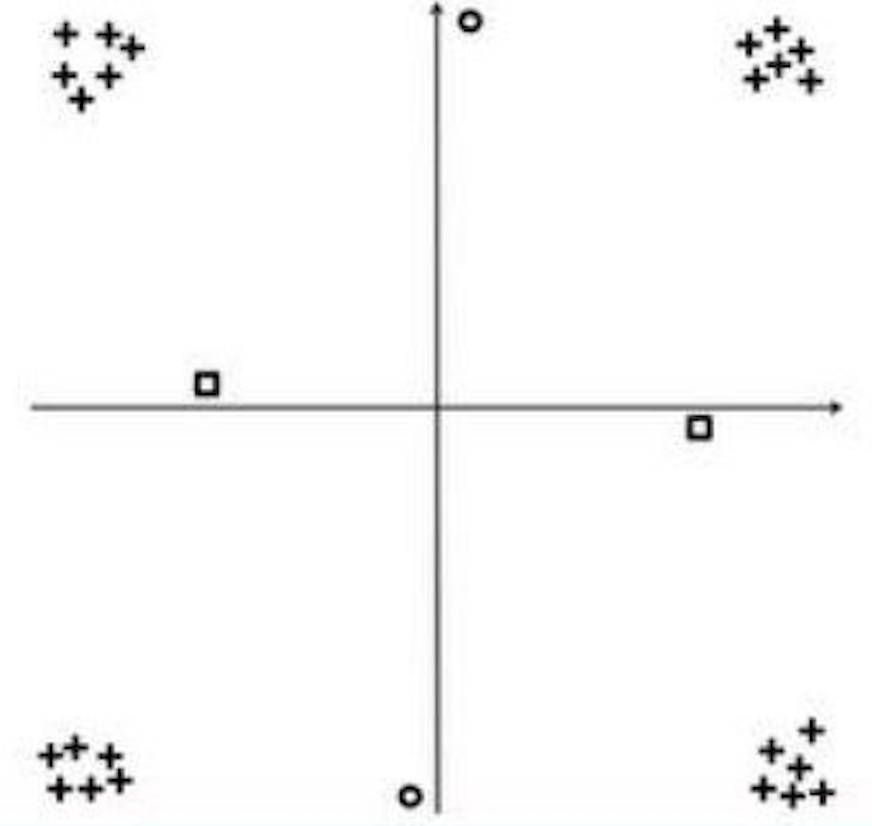
\includegraphics[width=0.6\textwidth,height=0.6\textheight,keepaspectratio]{images/graph_7_Sept_2021.png}
    \end{figure}

    \begin{solution}
        \begin{figure}[H]
            \centering
            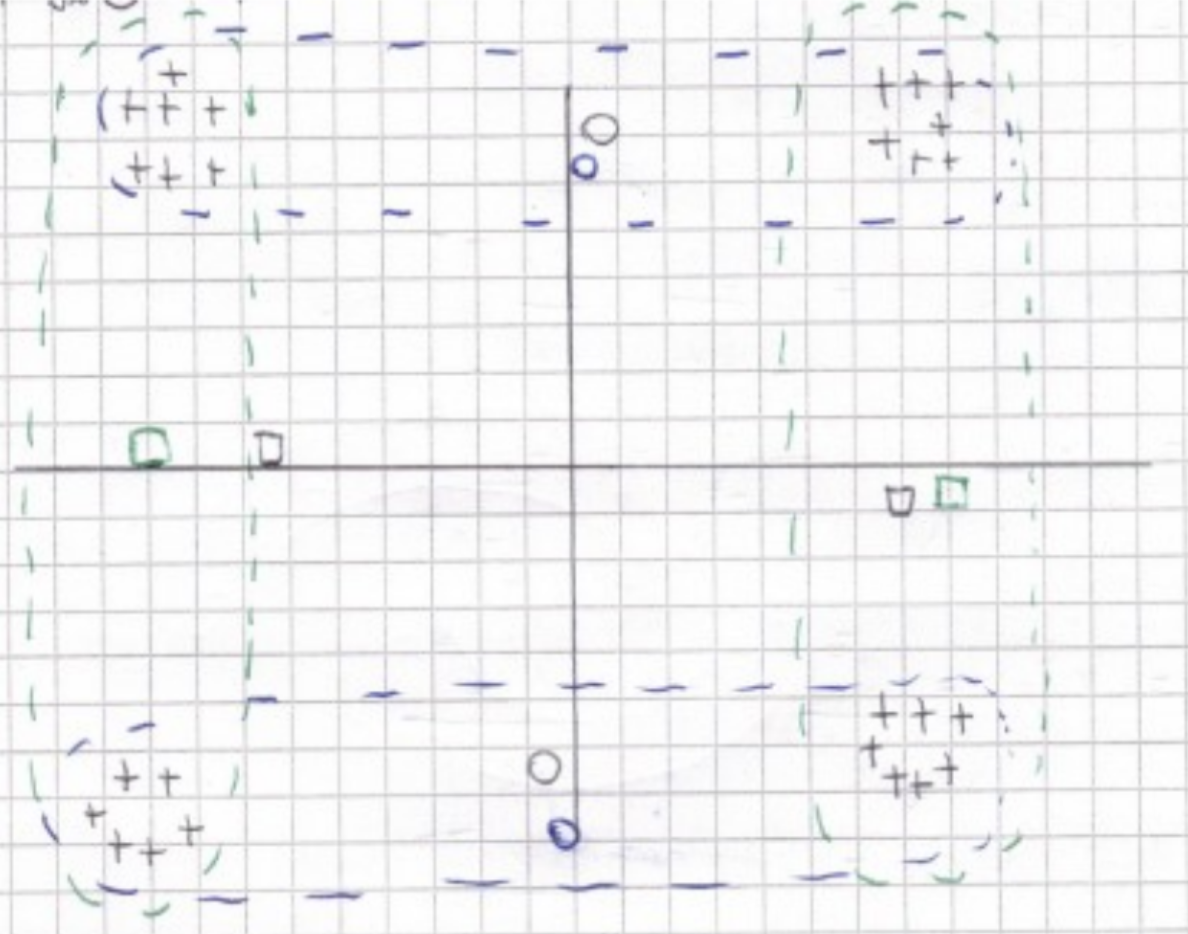
\includegraphics[width=0.6\textwidth,height=0.6\textheight,keepaspectratio]{images/solution_4_7_Sept_2021.png}
        \end{figure}

        There is no solution that is significantly better than the other one since the data consists of 4 groups of points that are essentially symmetric with respect to the origin, and the two solutions are just two different ways to group them into two groups. Also the coefficient silhouette of the two solutions is probably similar.
    \end{solution}
\end{enumerate}

%-----------------------------------------------------------------------------------------------

\chapter{6 July 2021}

\begin{figure}[H]
   \centering
   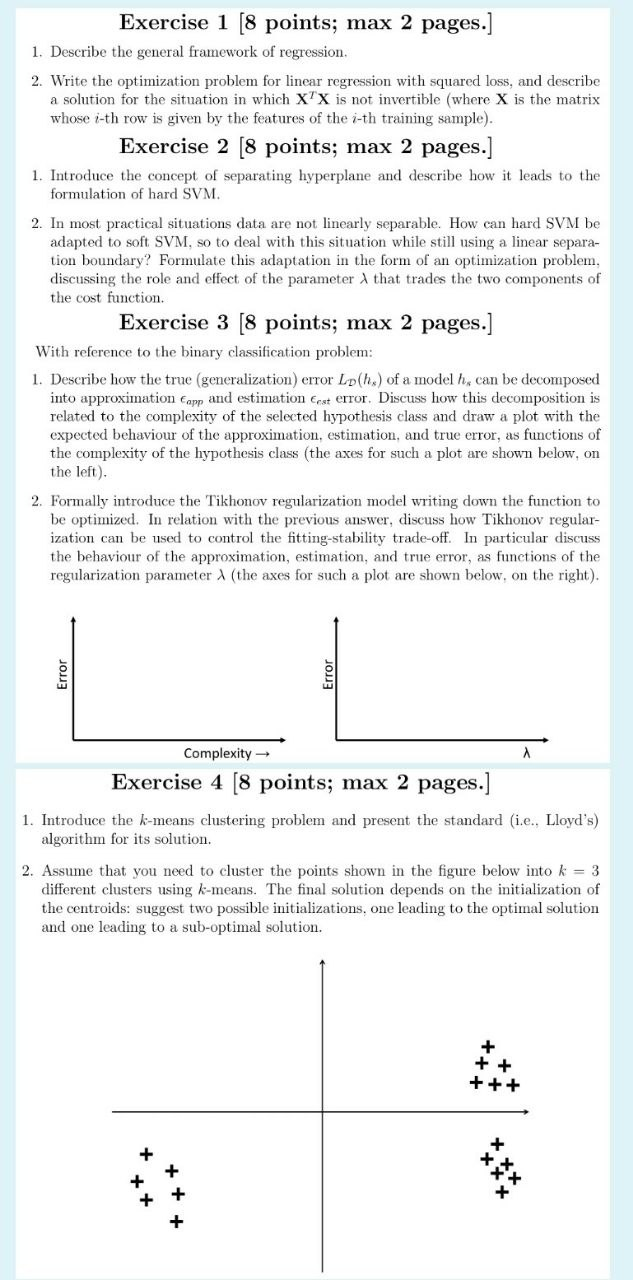
\includegraphics[width=0.8\textwidth,height=0.8\textheight,keepaspectratio]{images/6_Jul_2021.jpg}
\end{figure}

\clearpage
\section{Exercise 1}
\begin{enumerate}
\item Describe the general framework of regression.
    \begin{solution}
        Regression task is a supervised learning task with:
        
        \begin{itemize}
        \item Domain set $X$ which is the set of all possible objects to make predictions about, where a domain point $x \in X$ is called instance and is usually represented by a vector of features, usually is equal to $\mathbb{R}^d$
        
        \item Label set $Y = \mathbb{R}$
        \end{itemize}
        
        Given a training set $S = ((x_1, y_1) ... (x_m, y_m))$ with $x_i \in X, y_i \in Y$ $\forall i = 1,..,m$ we need to choose an hypothesis class H, which defines the possible models or classification rules, from which we can pick our model to make predictions, and a loss function $l: H \times Z \to \mathbb{R}^+$ where $Z = X \times Y$ that given an hypothesis provides a measure of how much we lose by predicting the value $h(\vec{x})$ for $\vec{x}$ instead of the correct value $y$.
        
        The goal is to find an hypothesis $\hat{h} \in H$ with low generalization error: $L_d(\hat{h}) = E_{z\sim D}[l(\hat{h},z)]$ where:
        
        \begin{itemize}
        \item $D$ is the unknown probability distribution over $Z$ from which $(x_i, y_i) \in S$ have been drawn (as independent samples).
        \end{itemize}
    \end{solution}
\clearpage
\item Write the optimization problem for linear regression with squared loss, and describe a solution for the situation in which $X^TX$ is not invertible (where $X$ is the matrix whose $i$-th row is given by the features of the $i$-th training sample).
    \begin{solution}

        The optimization problem for linear regression with squared loss can be described as follow:
        
        Given:
        \begin{itemize}
        \item $S = ((x_1, y_1) ... (x_m, y_m))$ with $x_i \in X, y_i \in Y$ $\forall i = 1,..,m$ training set
        \item $H = L_d = \{h_{\vec{w},b}: \mathbb{R}^d \to \mathbb{R}\}$ where $h_{\vec{w},b}(\vec{x}) = \langle \vec{w},\vec{x} \rangle + b$ be the hypothesis class
        \item $l(h, (\vec{x}, y)) = (h(\vec{x}) - y)^2 = (\langle \vec{w},\vec{x} \rangle + b - y)^2 = (\langle \vec{w}',\vec{x}' \rangle - y)^2$ if $\vec{w}' = [b, w_1, ..., w_m]$ and $x' = [1,x_1, ..., x_m]$ be the loss function
        \end{itemize}
        
        Then the function to be optimized is $\sum_{i=1}^m(\langle \vec{w}',\vec{x}'_i \rangle - y_i)^2$ therefore we obtain that $(X^TX)\vec{w} = X^T\vec{y}$
        
        Now if $X^TX$ is not invertible then we need to compute the generalized inverse of that matrix. So, let $A = X^TX$, the generalized inverse of $A$ is the matrix $A^+$ such that: $AA^+A = A$.
        To define $A^+$ we need to apply the following steps:
        
        \begin{itemize}
        \item Apply the eigenvalue decomposition to A and obtain $A = VDV^T$ where:
        \begin{enumerate}
        \item V is the matrix in which columns there are the eigenvectors normalized of A
        \item D is a diagonal matrix where in the diagonal there are the eigenvalues in the correspondence position of the correspondent eigenvector in V
        \end{enumerate}
        
        \item Finally define $A^+ = VD^+V^T$ where:
        \begin{enumerate}
        \item V is the matrix as above
        \item $D^+$ is defined as follows:
            $$d_{ij}^+ = \begin{cases}
            \frac{1}{d_{ij}} & \text{if } i = j \\
            0 & \text{otherwise}
            \end{cases}$$
            where $d_{ij}^+$ is the element in position $(i,j)$ of $D^+$ and $d_{ij}$ is the element in position $(i,j)$ of $D$
        \end{enumerate}
        \end{itemize}
    \end{solution}
\end{enumerate}

\section{Exercise 2}
\begin{enumerate}
\item Introduce the concept of separating hyperplane and describe how it leads to the formulation of hard SVM.
    \begin{solution}
        Given a binary classification problem where:
        \begin{itemize}
        \item Domain set $X$ which is the set of all possible objects to make predictions about, where a domain point $\vec{x} \in X$ is called instance and is usually represented by a vector of features
        \item Label set $Y = \{-1,+1\}$, that defines the set of all possible labels in this case the labels are only 2
        \item set $S = ((x_1, y_1) ... (x_m, y_m))$ with $x_i \in X, y_i \in Y$ $\forall i = 1,..,m$ is the so called training set
        \end{itemize}
        
        A separating hyperplane is an hyperplane that separates all the points of the training set $S$ into two parts, namely into two halfspaces which contains all and only the points that have either class -1 or +1.
        In case in which the training set $S$ is linearly separable, then there exists more than one such hyperplane and in particular we can define the optimal as the one that maximizes the margin i.e. the distance between the hyperplane and the closest points in $S$ to him.
        
        The optimal separating hyperplane introduced above is exactly the solution computed by the SVM when data are linearly separable. In particular if we define:
        \begin{itemize}
        \item hyperplane as: $L = \{v :\langle \vec{w}, \vec{v} \rangle +b = 0\}$
        \item distance between a point $x$ and $L$: $d(x,L) = \min \{|\vec{x} - \vec{v}|: v \in L\}$
        \end{itemize}
        
        Then the optimal separating hyperplane can be computed as:
        $$\argmax_{(\vec{w},b): \|\vec{w}\|=1 \; i\in\{1,...,m\}} \min |\langle \vec{w},\vec{x}_i \rangle +b| \text{ subject to: } \forall i \; y_i(\langle \vec{w},\vec{x}_i \rangle +b)$$
        
        Which corresponds to the formulation of the Hard-SVM, namely the formulation of the SVM when data are linearly separable.
    \end{solution}
\clearpage
\item In most practical situations data are not linearly separable. How can hard SVM be adapted to soft SVM, so to deal with this situation while still using a linear separation boundary? Formulate this adaptation in the form of an optimization problem, discussing the role and effect of the parameter $\lambda$ that trades the two components of the cost function.
    \begin{solution}
        Soft-SVM is similar to Hard-SVM, but can be used also when training data is not linearly separable (i.e., the training data cannot be perfectly classified with a linear model). Soft-SVM finds a model of large margin while allowing the training set to be inside the margin or wrongly classified. This is obtained by adding slack variables $\xi_i$ to the constraints of hard SVM. The constraint for soft-SVM are then:
        \begin{itemize}
        \item $\xi_i \geq 0$ for each $i = 1,...,m$
        \item $y_i(\langle \vec{w},\vec{x}_i \rangle +b) \geq 1 - \xi_i$ for each $(x_i,y_i)$ $i = 1,...,m$ in the training set where $\vec{w}$ and $b$ defines the model.
        \end{itemize}
        
        The interpretation of $\xi_i$ is the following:
        \begin{itemize}
        \item if $\xi_i = 0$ then $\vec{x}_i$ is correctly classified and outside the margin;
        \item if $0 < \xi_i < 1$ then $\vec{x}_i$ is correctly classified and inside the margin;
        \item if $\xi_i \geq 1$ then $\vec{x}_i$ is wrongly classified.
        \end{itemize}
        
        The function optimized by soft-SVM consider both the margin and the "violation" of the hard-SVM given by $\xi_i$.
        
        Therefore the optimization problem for soft-SVM can be described as follows:
        
        Input: $S = ((\vec{x}_1, y_1) ... (\vec{x}_m, y_m))$ and parameter $\lambda > 0$
        
        Goal: $\min_{\vec{w},b,\vec{\xi}} \lambda\|\vec{w}\|^2 + \frac{1}{m}\sum_{i=1}^m \xi_i$
        
        Output: $\vec{w}, b, \vec{\xi}$
        
        The parameter lambda controls the tradeoff between an high margin with several points misclassified and a small margin with most of the points correctly classified in particular, if $\lambda \approx 0$ then, soft-SVM will produce a model that tries to be as similar as possible as the one produced by hard-SVM namely, it tries to classified as many as possible points correctly. On the other hand, if $\lambda \gg 0$ then, soft-SVM cares only about maximizing the margin therefore, it produces a model that has most of the points misclassified but it has an high margin.
    \end{solution}
\end{enumerate}

\section{Exercise 3}
With reference to the binary classification problem:
\begin{enumerate}
\item Describe how the true (generalization) error $L_D(h_s)$ of a model $h_s$ can be decomposed into approximation $\epsilon_{app}$ and estimation $\epsilon_{est}$ error. Discuss how this decomposition is related to the complexity of the selected hypothesis class and draw a plot with the expected behaviour of the approximation, estimation, and true error, as functions of the complexity of the hypothesis class (the axes for such a plot are shown below, on the left).
    \begin{solution}
        The generalization error $L_D(h_S)$ can be decomposed into $L_D(h_S) = \epsilon_{app} + \epsilon_{est}$ where $\epsilon_{app} = \min_{h\in H}L_D(h)$ and $\epsilon_{est} = L_D(h_S) - \min_{h\in H}L_D(h)$.
        
        In words:
        \begin{itemize}
        \item $\epsilon_{app}$ = approximation error: is the minimum risk achievable by a predictor in the hypothesis class.
        \item $\epsilon_{est}$ = estimation error: is the difference between the approximation error and the error achieved by the ERM predictor.
        \end{itemize}
        
        Therefore if we plot in a graph those two error and the $L_D(h_S)$ as functions of the complexity we obtain that:
        \begin{itemize}
        \item $\epsilon_{app}$: will decrese if the complexity decreases if complexity increases
        \item $\epsilon_{est}$: will increase if the complexity increases  
        \item $L_D(h_S)$: has a "bell" behaviour
        \end{itemize}
        
        The graph is the following:
        
        \begin{figure}[H]
            \centering
            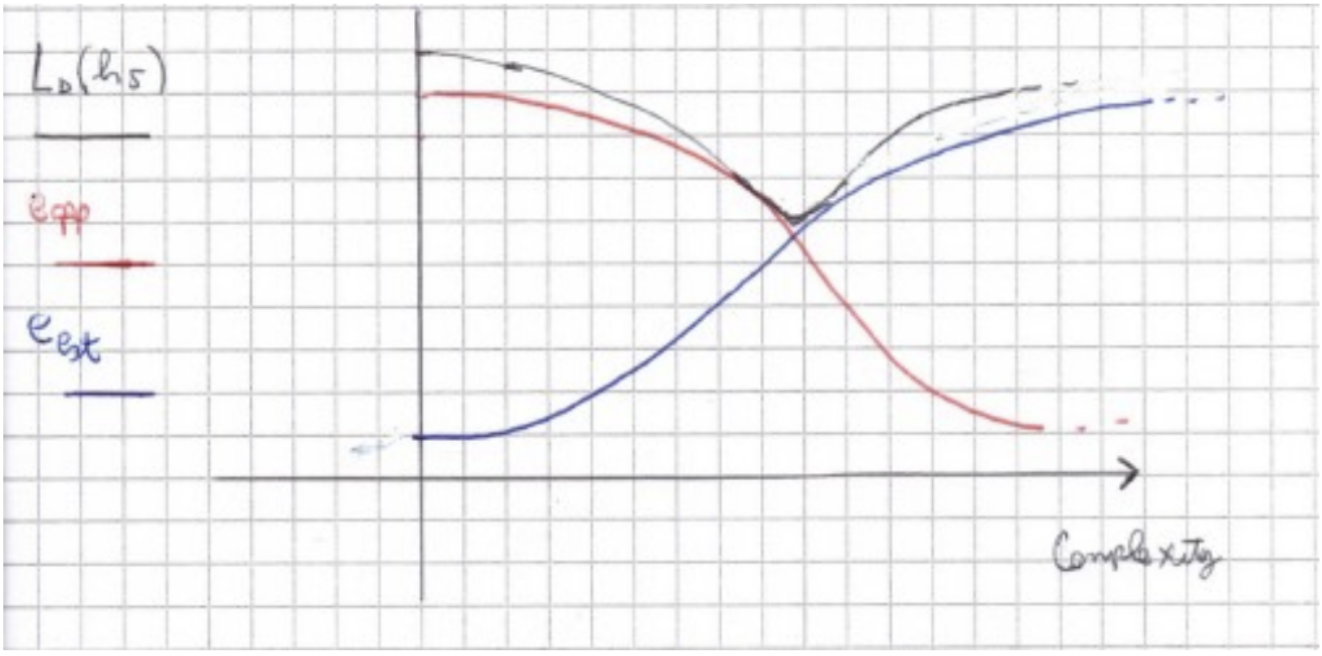
\includegraphics[width=0.6\textwidth,height=0.6\textheight,keepaspectratio]{images/1_3_6_Jul_2021.png}
         \end{figure}
        
        Notice that a low complexity hypothesis class corresponds to a underfitting situation while a high complexity class corresponds to a overfitting situation.
    \end{solution}
    
\item Formally introduce the Tikhonov regularization model writing down the function to be optimized. In relation with the previous answer, discuss how Tikhonov regularization can be used to control the fitting-stability trade-off. In particular discuss the behaviour of the approximation, estimation, and true error, as functions of the regularization parameter $\lambda$ (the axes for such a plot are shown below, on the right).
\begin{figure}[H]
    \centering
    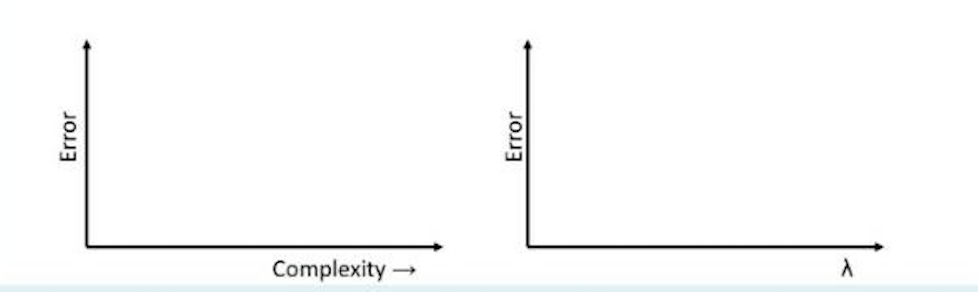
\includegraphics[width=0.6\textwidth,height=0.6\textheight,keepaspectratio]{images/3_Jul_2021.png}
 \end{figure}
    \begin{solution}
        Tikhonov regularization is the Regularized loss minimization paradigm with regularization function $R(\vec{w}) = \lambda\|\vec{w}\|^2$ where $\lambda > 0$ and $\|\vec{w}\|^2$ is the $l_2$ norm of the vector $\vec{w}$.
        
        Therefore the function to be optimized, i.e. minimized is the following: $\argmin_{\vec{w}}(L_S(\vec{w}) + \lambda\|\vec{w}\|^2)$ where $L_S(\vec{w})$ is the training error and $S$ is the training set.
        
        Notice that $\|\vec{w}\|^2$ measures the complexity of the hypothesis $\vec{w}$, while $\lambda$ is the parameter used to tradeoff the empirical risk and the complexity of the model.
        
        Now, the behavior of the $\epsilon_{app}$, $\epsilon_{est}$ and $L_D(h_S)$ in terms of the parameter $\lambda$ is the following:
        \begin{itemize}
        \item $\epsilon_{app}$ will increase if $\lambda$ increases because with a low $\lambda$ we have a complex hypothesis class
        \item $\epsilon_{est}$ will decrease if $\lambda$ increases because with an high $\lambda$ we have a low-complexity hypothesis class
        \item $L_D(h_S)$: has a "bell" behaviour
        \end{itemize}
        
        The graph is the following:
        
        \begin{figure}[H]
            \centering
            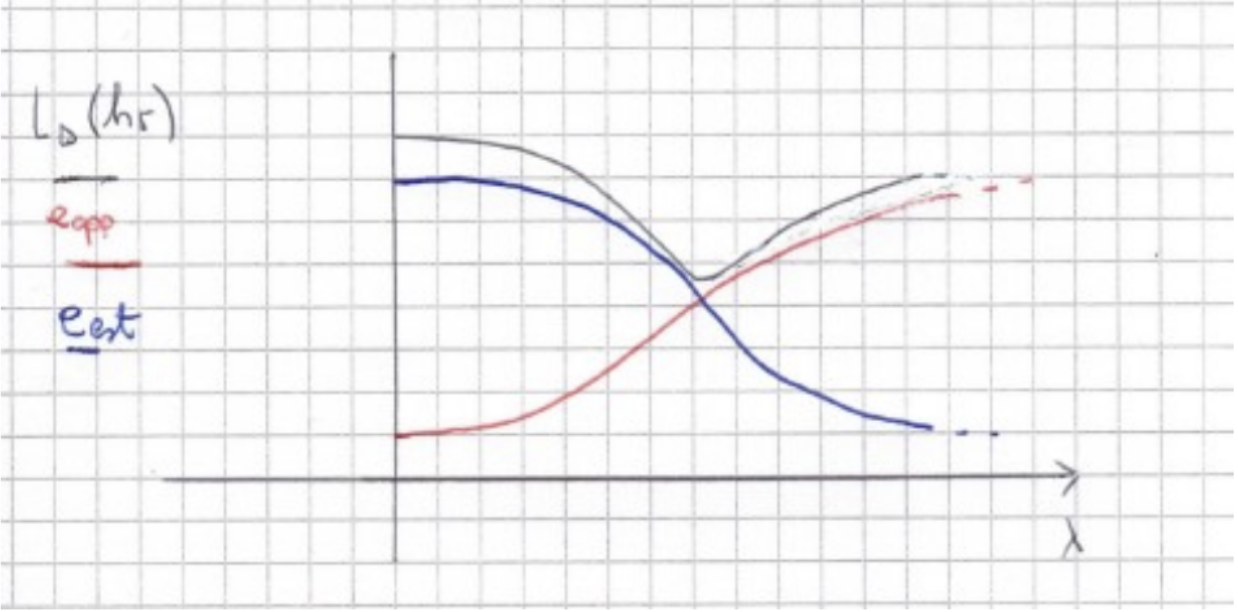
\includegraphics[width=0.6\textwidth,height=0.6\textheight,keepaspectratio]{images/2_3_6_Jul_2021.png}
         \end{figure}
    \end{solution}
\end{enumerate}

\section{Exercise 4}
\begin{enumerate}
\item Introduce the k-means clustering problem and present the standard (i.e., Lloyd's) algorithm for its solution.
    \begin{solution}
        K-means is a cost minimization clustering problem. Let $X \subseteq X'$ be the set of points to be clustered with $X = \{\vec{x}_1,...,\vec{x}_m\}$ while $X'$ is the space of possible points that we assume to be in $\mathbb{R}^d$ (i.e $X' = \mathbb{R}^d$).
        Let $k \in \mathbb{N}^+$ be the number of clusters, that is, with $X$, the input of the problem.
        Let $d(.)$ be a distance function: $d(\vec{x},\vec{x'}) = \|\vec{x} - \vec{x'}\|$.
        
        The goal is to find:
        \begin{itemize}
        \item A partition $C = (C_1,..,C_k)$ of $X$
        \item Centroids $\vec{\mu}_1,...,\vec{\mu}_k$ of $C_1,..,C_k$ respectively
        \end{itemize}
        
        That minimizes the k-means cost function: $\sum_{i=1}^k \sum_{\vec{x}\in C_i} d(\vec{x},\vec{\mu}_i)^2$
        
        To find the solution of this problem we can use an heuristic algorithm called Lloyd's Algorithm. Such algorithm works as follows:
        
        Input: data points $X = \{\vec{x}_1,...,\vec{x}_m\}$ and $k \in \mathbb{N}^+$\\
        Output: $C = (C_1,...,C_k)$ of $X$ and centroids $\vec{\mu}_1,...,\vec{\mu}_k$ of $C_1,...,C_k$ respectively
        
        To produce such things the algorithm works as follows:
        \begin{itemize}
        \item Randomly initialize the centroids $\vec{\mu}_1,...,\vec{\mu}_k$
        \item Until the convergence is not reached iteratively repeats the following steps:
        \begin{enumerate}
        \item Compute each cluster $C_i$ by associating the points to him that are closer to its centroid compared to others centroids.
        \item Compute the new centroids for the next iterations.
        \item If the convergence is reached then the output described above will be returned.
        \end{enumerate}
        \end{itemize}
        
        The pseudocode for such algorithm is the following:
        
        \begin{algorithmic}[1]
        \State Randomly choose $\vec{\mu}_1^0,...,\vec{\mu}_k^0$
        \For{$t \leftarrow 0,...$ do}
        \For{$i = 1,...,k$}
            \State $C_i \gets \{\vec{x} \in X : i = \argmin_j d(\vec{x},\vec{\mu}_j^t)\}$
        \EndFor
        \For{$i = 1,...,k$}
            \State $\vec{\mu}_i^{t+1} = \frac{1}{|C_i|}\sum_{\vec{x}\in C_i} \vec{x}$
        \EndFor
        \If{convergence reached}
            \State \Return $C = (C_1,...,C_k), \vec{\mu}_1^{t+1},...,\vec{\mu}_k^{t+1}$
        \EndIf
        \EndFor
        \end{algorithmic}
        
        The convergence criteria that can be used for such algorithm are the following:
        \begin{itemize}
        \item The k-means objective function is no lower than the k-means objective function at the next iteration
        \item $\sum_{i=1}^k d(\vec{\mu}_i^{t+1},\vec{\mu}_i^t) \leq \varepsilon$
        \item $\max_{1\leq i\leq k}d(\vec{\mu}_i^{t+1},\vec{\mu}_i^t) \leq \varepsilon$
        \end{itemize}
        
        Note that if the first criteria is used then, the algorithm will always converge.
        
        The time complexity is $O(tkmd)$ where $O(kmd)$ is due to the assignments of the points, while $O(md)$ is due to the computation of the centroids. Therefore the complexity depends on t which is the number of iterations of the algorithm.
    \end{solution}
\clearpage
\item Assume that you need to cluster the points shown in the figure below into $k = 3$ different clusters using k-means. The final solution depends on the initialization of the centroids; suggest two possible initializations, one leading to the optimal solution and one leading to a sub-optimal solution.
\begin{figure}[H]
    \centering
    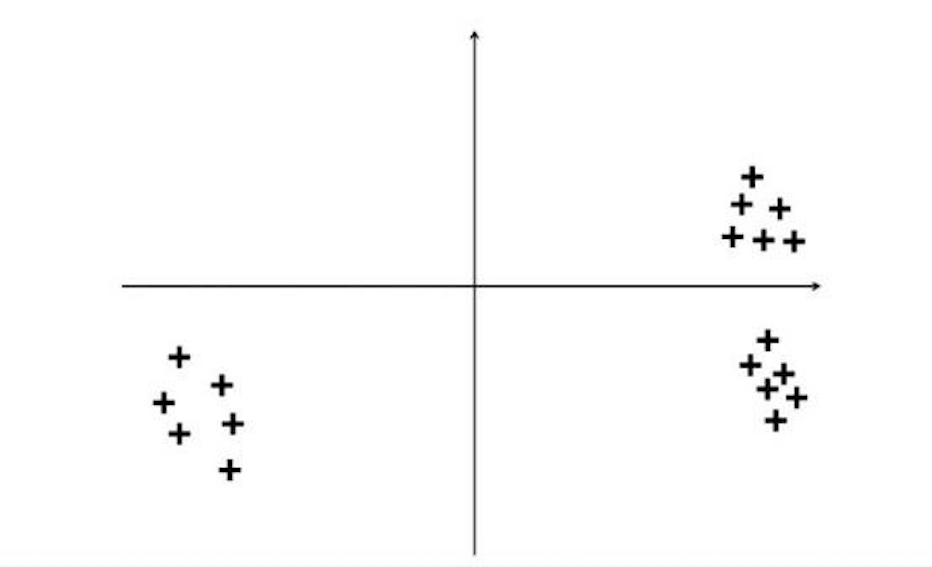
\includegraphics[width=0.7\textwidth,height=0.7\textheight,keepaspectratio]{images/4_Jul_2021.png}
 \end{figure}
    \begin{solution}
        \begin{figure}[H]
            \centering
            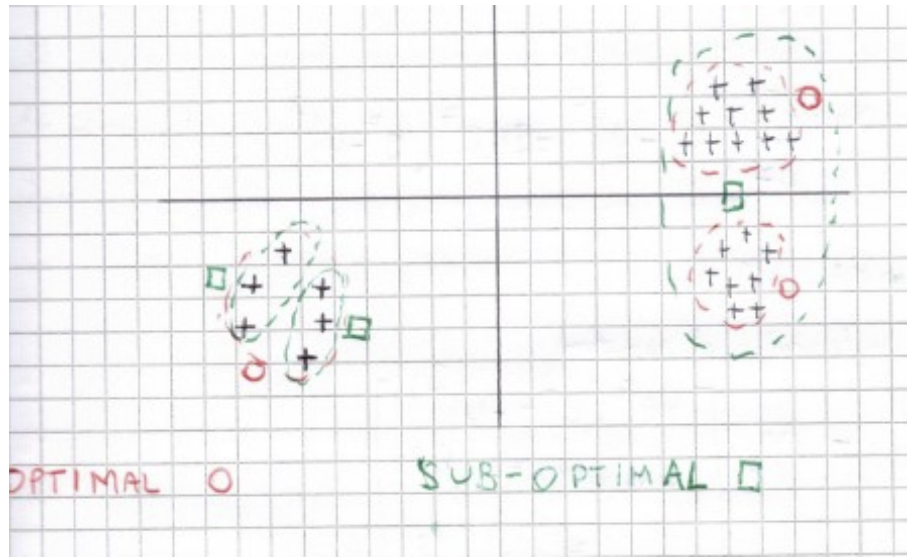
\includegraphics[width=0.8\textwidth,height=0.8\textheight,keepaspectratio]{images/2_4_6_Jul_2021.png}
         \end{figure}
    \end{solution}
\end{enumerate}

%-----------------------------------------------------------------------------------------------

\chapter{28 January 2021}

\begin{figure}[H]
    \centering
    \begin{minipage}{0.45\textwidth}
        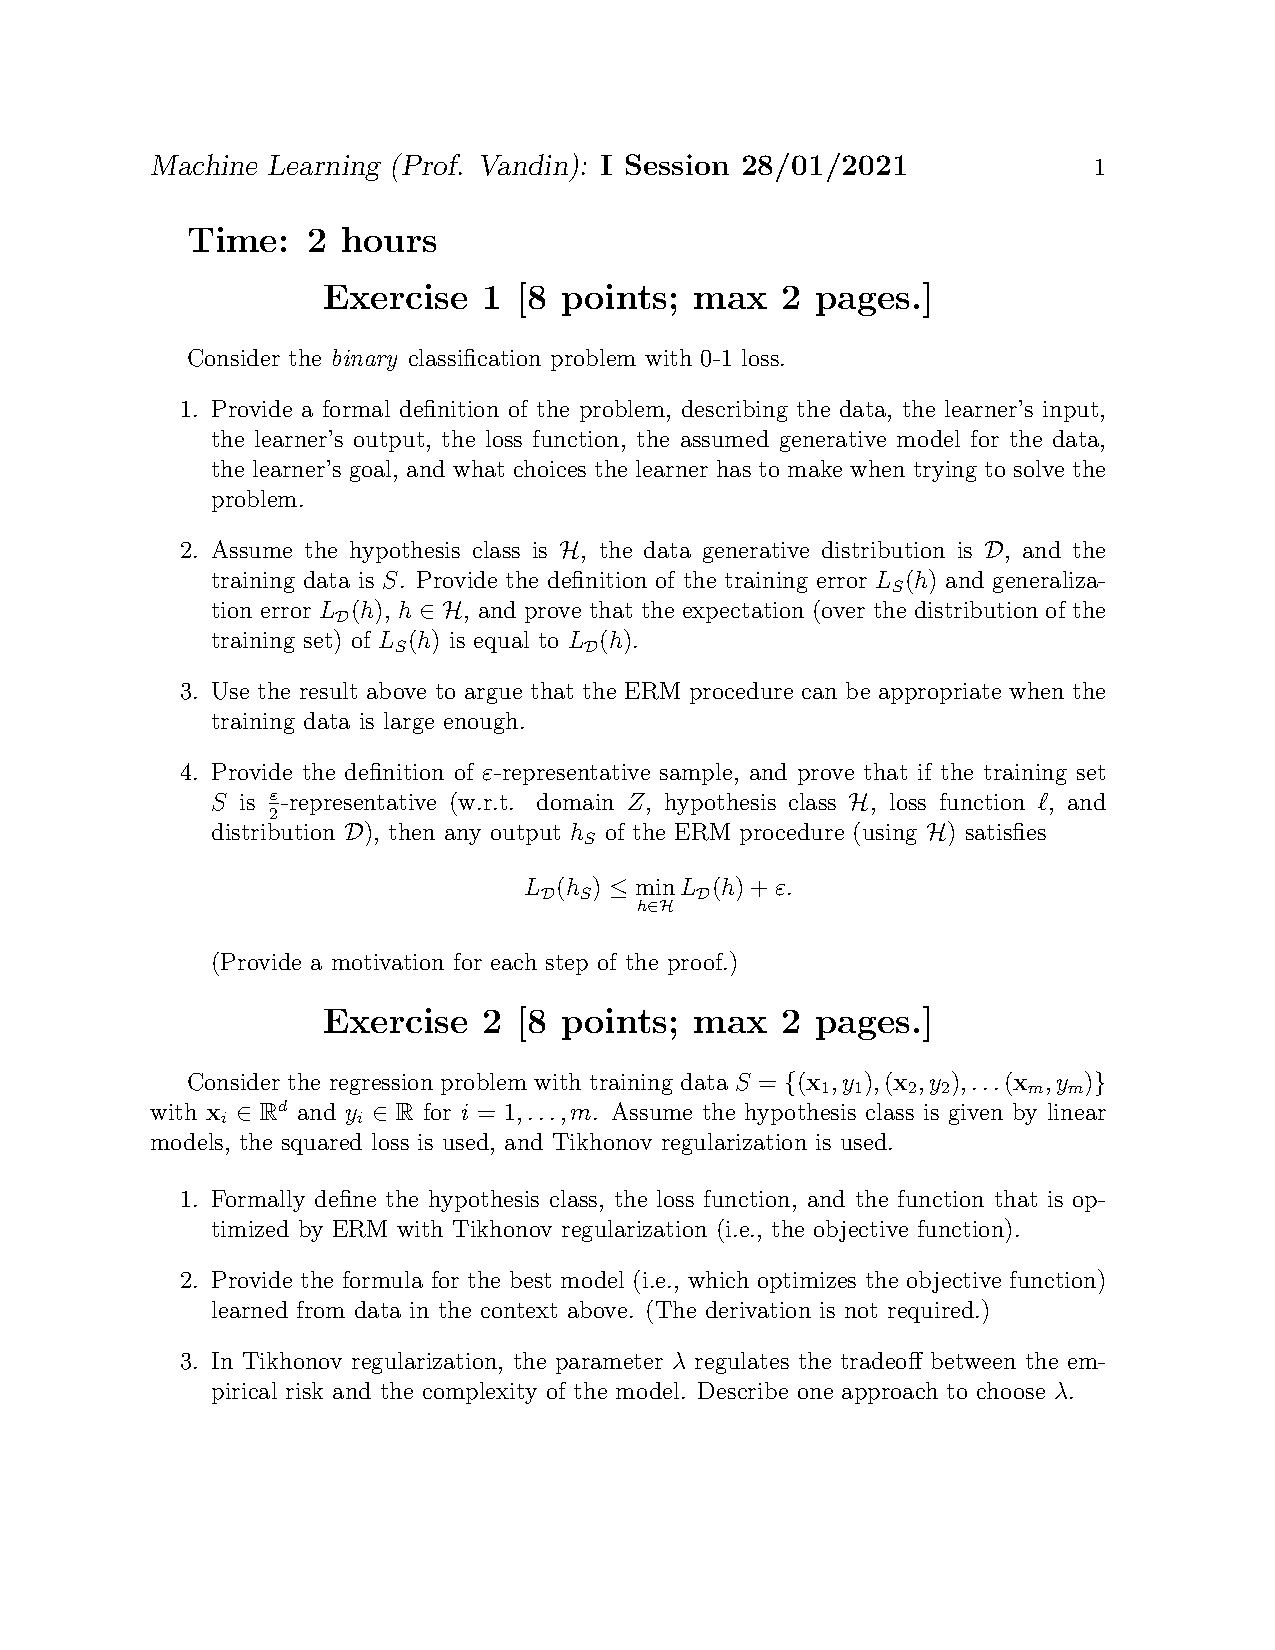
\includegraphics[width=\textwidth,page=1]{images/28_Jan_2021.pdf}
    \end{minipage}
    \hfill
    \begin{minipage}{0.45\textwidth}
        \includegraphics[width=\textwidth,page=2]{images/28_Jan_2021.pdf}
    \end{minipage}
    
    \vspace{1cm}
    
    \begin{minipage}{0.45\textwidth}
        \includegraphics[width=\textwidth,page=3]{images/28_Jan_2021.pdf}
    \end{minipage}
\end{figure}

\clearpage
\section{Exercise 1}
Consider the binary classification problem with 0-1 loss.
\begin{enumerate}
\item Provide a formal definition of the problem, describing the data, the learner's input, the learner's output, the loss function, the assumed generative model for the data, the learner's goal, and what choices the learner has to make when trying to solve the problem.
    \begin{solution}
        The binary classification problem with 0-1 loss is a supervised learning problem with:
        \begin{itemize}
        \item Domain set $X$ which is the set of all possible objects to make predictions about, where a domain point $\vec{x} \in X$ is called instance and is usually represented by a vector of features
        \item Label set $Y = \{-1,+1\}$, that defines the set of all possible labels in this case the labels are only 2
        \end{itemize}
        
        Given a training set $S = ((x_1, y_1) ... (x_m, y_m))$ with $x_i \in X, y_i \in Y$ $\forall i = 1,..,m$ we need to choose an hypothesis class H, which defines the possible models or classification rules, from which we can pick our model to make predictions, and a loss function $l: H \times Z \to \mathbb{R}^+$ where $Z = X \times Y$ that given an hypothesis provides a measure of how much we lose by predicting the value $h(\vec{x})$ for $\vec{x}$ instead of the correct value $y$.
        
        In particular in the case of 0-1 loss the function is exactly the following:
        $$l(h, (\vec{x},y)) = \begin{cases}
        1 \text{ if } h(\vec{x}) \neq y \\
        0 \text{ if } h(\vec{x}) = y
        \end{cases}$$
        
        The goal is to find an hypothesis $\hat{h} \in H$ with low generalization error: $L_d(\hat{h}) = E_{z\sim D}[l(\hat{h},z)]$ where:
        \begin{itemize}
        \item $D$ is the unknown probability distribution over $Z$ from which $(x_i, y_i) \in S$ have been drawn (as independent samples).
        \end{itemize}
    \end{solution}

\item Assume the hypothesis class is $\mathcal{H}$, the data generative distribution is $\mathcal{D}$, and the training data is $S$. Provide the definition of the training error $L_S(h)$ and generalization error $L_D(h)$, $h \in \mathcal{H}$, and prove that the expectation (over the distribution of the training set) of $L_S(h)$ is equal to $L_D(h)$.
    \begin{solution}
        Let:
        \begin{itemize}
        \item $X$ be the domain set, which is the set of all possible objects to make predictions about, where a domain point $\vec{x} \in X$ is called instance and is usually represented by a vector of features
        \item $Y$ be the label set that defines the set of all possible labels
        \item $S = ((\vec{x}_1, y_1) ... (\vec{x}_m, y_m))$ with $x_i \in X, y_i \in Y$ $\forall i = 1,..,m$ be the training set
        \item $l: H\times Z \to \mathbb{R}^+$ where $Z = X\times Y$ be the loss function namely a function that given an hypothesis provides a measure of how much we lose by predicting the value $h(\vec{x})$ for $\vec{x}$ instead of the
        \item $D$ be the unknown distribution
        \item $H$ be the hypothesis class
        \end{itemize}
        
        We define the training error as: $L_S(h) = \frac{1}{m}\sum_{i=1}^m l(h, (\vec{x}_i,y_i))$.
        
        We define the generalization error as: $L_d(h) = E_{z\sim D}[l(h,z)]$ where $z = (\vec{x}, y)$
        
        \begin{align*}
        E[L_s(h)] &= E\left[\frac{1}{m}\sum_{i=1}^m l(h, (\vec{x}_i,y_i))\right] \\
        &= \frac{1}{m}\sum_{i=1}^m E[l(h, (\vec{x}_i,y_i))] \\
        &= \frac{1}{m}\sum_{i=1}^m L_d(h) \\
        &= L_d(h)
        \end{align*}
    \end{solution}
\item Use the result above to argue that the ERM procedure can be appropriate when the training data is large enough.
    \begin{solution}
        $L_s(h)$ is the probability that a pair $(\vec{x}_i,y_i)$ taken uniformly at random from $S$ the event $h(\vec{x}_i) \neq y_i$. That means, if we compute $E[L_s(h)]$, then it is equal to $L_d(h)$ if we have enough data because $S$ is taken from $D$. Therefore $L_s(h) \approx L_d(h)$ because with enough data $E[L_s(h)] = L_d(h)$.
    \end{solution}
    $$L_D(h_S) \leq \min_{h\in\mathcal{H}} L_D(h) + \varepsilon.$$
\item Provide the definition of $\varepsilon$-representative sample, and prove that if the training set $S$ is $\frac{\varepsilon}{2}$-representative (w.r.t. domain $Z$, hypothesis class $\mathcal{H}$, loss function $\ell$, and distribution $\mathcal{D}$), then any output $h_S$ of the ERM procedure (using $\mathcal{H}$) satisfies
(Provide a motivation for each step of the proof.)
    \begin{solution}
        A set $S$ is $\varepsilon$-representative (with respect to domain $Z$, hypothesis class $H$, loss function $l$ and distribution $D$ if: 
        $$\forall h \in H \quad |L_S(h) - L_d(h)| \leq \varepsilon$$
    \end{solution}
\end{enumerate}

\section{Exercise 2}
Consider the regression problem with training data $S = \{(\mathbf{x}_1, y_1), (\mathbf{x}_2, y_2), \ldots (\mathbf{x}_m, y_m)\}$ with $\mathbf{x}_i \in \mathbb{R}^d$ and $y_i \in \mathbb{R}$ for $i = 1,\ldots,m$. Assume the hypothesis class is given by linear models, the squared loss is used, and Tikhonov regularization is used.
\begin{enumerate}
\item Formally define the hypothesis class, the loss function, and the function that is optimized by ERM with Tikhonov regularization (i.e., the objective function).
    \begin{solution}
        With the assumption made we have that:
        \begin{itemize}
        \item $H$: the hypothesis class is exactly equal to $L_d = \{h_{\vec{w},b}: \mathbb{R}^d \to \mathbb{R}\}$ where $h_{\vec{w},b}(\vec{x}) = \langle \vec{w},\vec{x} \rangle +b$
        \item $l$: the loss function is exactly equal to $l: H\times Z \to \mathbb{R}^+$ where $Z = X\times Y$ such that $l(h,(\vec{x},y)) = (h(\vec{x}) - y)^2 = (\langle \vec{w},\vec{x} \rangle + b - y)^2 = (\langle \vec{w}',\vec{x}' \rangle - y)^2$ if $\vec{w}' = [b,w_1,...,w_m]$ and $\vec{x}' = [1,x_1,...,x_m]$
        \item The function to be optimized becomes: $\lambda\|\vec{w}\|^2 + \sum_{i=1}^m(\langle \vec{w}',\vec{x}'_i \rangle - y_i)^2$
        \end{itemize}
    \end{solution}
\item Provide the formula for the best model (i.e., which optimizes the objective function) learned from data in the context above. (The derivation is not required.)
    \begin{solution}
        The formula to compute the best model with the previous assumption is $\vec{w} = (\lambda I + X^TX)^{-1}X^T\vec{y}$ where:
        
        $$X = \begin{bmatrix} 
        \vec{x}'_1 \\
        \vdots \\
        \vdots \\
        \vec{x}'_m
        \end{bmatrix} \text{ and } \vec{y} = \begin{bmatrix}
        y_1 \\
        \vdots \\
        \vdots \\
        y_m
        \end{bmatrix}$$
    \end{solution}
\item In Tikhonov regularization, the parameter $\lambda$ regulates the tradeoff between the empirical risk and the complexity of the model. Describe one approach to choose $\lambda$.
    \begin{solution}
        A possible strategy to estimate the parameter $\lambda$ is to use cross-validation. Therefore recalling $\lambda$, $\vartheta$, we can apply the cross validation method.
        
        To be more precise, cross validation consists in a way to select a value of a parameter $\vartheta$ by understanding what is the best value that such parameter can assume with the data we have.
        To do so, we split the dataset into k different folds of size m/k (this quantity is supposed to be integer). Then for each value of the parameter $\vartheta$ we find the best model for all the possible k-1 folds that we can select. In addition to that, we compute the average error of each parameter as the average of the errors on the folds left out, and when we have repeated such procedure for all the values of the parameters, then we select the optimal one by choosing the one that minimizes the error computed for each parameter. To conclude, we train our model on all the dataset with the parameter found.
        
        The pseudo code is the following:
        
        \begin{algorithmic}[1]
        \State Input: $S = ((\vec{x}_1,y_1) ... (\vec{x}_m,y_m))$; set of parameters $\Theta$; integer k; learning algorithm A
        \State Split $S$ into $S_1,...,S_k$
        \For{$\vartheta \in \Theta$}
        \For{i = 1 ... k}
            \State $h_{i,\vartheta} = A(S\setminus S_i; \vartheta)$
        \EndFor
        \State $error(\vartheta) = \frac{1}{k}\sum_{i=1}^k L_{S_i}(h_{i,\vartheta})$
        \EndFor
        \State Output: $\vartheta^* = \argmin_\vartheta(error(\vartheta))$
        \State \hspace{35pt} $h_{\vartheta^*} = A(S; \vartheta^*)$
        \end{algorithmic}
    \end{solution}
\end{enumerate}

\section{Exercise 3}
Consider the regression problem, with training data $S = \{(\mathbf{x}_1, y_1), (\mathbf{x}_2, y_2), \ldots (\mathbf{x}_m, y_m)\}$ with $\mathbf{x}_i = [x_{i,1}, x_{i,2}] \in \mathbb{R}^2$ and $y_i \in \mathbb{R}$ for $i = 1,\ldots,m$.

Assume the hypothesis class $\mathcal{H}$ is given by the simple neural network with the architecture described in the figure below, where $w_0, w_1, w_2$ are the edges' weights.

\begin{figure}[H]
    \centering
    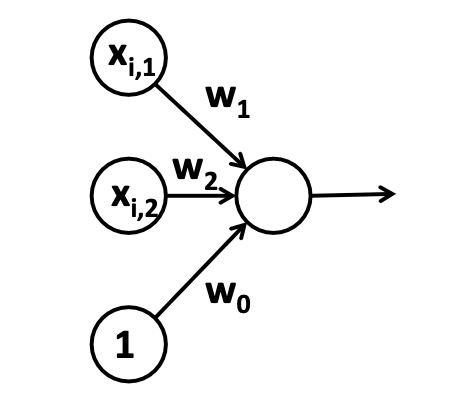
\includegraphics[width=0.4\textwidth,height=0.4\textheight,keepaspectratio]{images/3_28_Jan_2021.png}
 \end{figure}

Assume the activation function for the output node is $\sigma(z) = e^z$ (the final prediction is the output of the output node), and the loss function is $\ell(h, (\mathbf{x}, y)) = (h(\mathbf{x}) - y)^4$.
\begin{enumerate}
\item Derive a closed-form expression for the hypotheses in $\mathcal{H}$.
    \begin{solution}
        The closed-form expression for hypotheses in $\mathcal{H}$ is:
        
        $H_{V,E,e^z,w} = \{h_{V,E,e^z,w}: \mathbb{R}^2 \to \mathbb{R} \text{ such that w is a mapping from E to }\mathbb{R}\}$
        
        where:
        $$h_{V,E,e^z,w}(\vec{x}) = e^{(w_0 + w_1x_1 + w_2x_2)}$$
    \end{solution}

\item Describe the stochastic gradient descent (SGD) algorithm (in general). What is the main advantage of SGD with respect to the gradient descent algorithm?
    \begin{solution}
        The Stochastic Gradient Descent (SGD for short) algorithm is a general approach to minimize a differentiable convex function $f(\vec{w})$ where $f(\vec{w}): \mathbb{R}^d \to \mathbb{R}$.
        
        To do so, we update the current solution vector $\vec{w}^{(t)}$ as the following formula:
        \begin{itemize}
        \item Choose a vector $\vec{v}^{(t)}$ at random such that: $E[\vec{v}^{(t)}|\vec{w}^{(t)}] \in \nabla f(\vec{w})$
        \item $\vec{w}^{(t+1)} = \vec{w}^{(t)} - \eta\vec{v}^{(t)}$
        \end{itemize}
        
        Which can be translated, if $f(\vec{w}) = L_S(\vec{w})$ to:
        \begin{itemize}
        \item Pick a random point $(\vec{x}_i, y_i)$ uniformly at random from the training set $S = ((\vec{x}_1,y_1) ... (\vec{x}_m,y_m))$
        \item Compute $\vec{v}^{(t)} = \nabla l(h, (\vec{x}_i,y_i))$
        \item $\vec{w}^{(t+1)} = \vec{w}^{(t)} - \eta\vec{v}^{(t)}$
        \end{itemize}
        
        Therefore the main advantage is that with stochastic gradient descent we compute the gradient of a much less complicated function, (i.e. the gradient of the loss function), compare to the gradient descent algorithm because, in such algorithm we need to update $\vec{w}^{(t)}$ with the following rule:
        $\vec{w}^{(t+1)} = \vec{w}^{(t)} - \eta\nabla f(\vec{w})$. In addition it can be used also when $f(\vec{w}) = L_S(\vec{w}) + R(\vec{w})$.
    \end{solution}
\item Write the SGD update for learning a model from the hypothesis class $\mathcal{H}$ above.
    \begin{solution}
        In general, for stochastic gradient descent (SGD) let $\vec{w}^{(t)}$ be the weights optimize the model at iteration t. The update rule is given by:
        
        \begin{itemize}
        \item Pick $(\vec{x}_i,y_i) \in S$ uniformly at random
        \item $\vec{w}^{(t+1)} \leftarrow \vec{w}^{(t)} - \eta \nabla l(h,(\vec{x}_i,y_i))$
        \end{itemize}
        
        We need to compute the gradient for a specific model class and loss. In our case each model in our model class is a function:
        
        $$h(\vec{x}) = e^{w_0 + w_1x_1 + w_2x_2}$$
        
        Therefore:
        $$\nabla l(h,(\vec{x}_i,y)) = \begin{bmatrix}
        \frac{\partial l}{\partial w_0} \\
        \frac{\partial l}{\partial w_1} \\
        \frac{\partial l}{\partial w_2}
        \end{bmatrix} \text{ where } z = w_0 + w_1x_1 + w_2x_2$$
        
        $$\frac{\partial l}{\partial w_0} = \frac{\partial l}{\partial z} \cdot \frac{\partial z}{\partial w_0} = 4(e^z-y)^3 \cdot e^z$$
        
        $$\frac{\partial l}{\partial w_1} = \frac{\partial l}{\partial z} \cdot \frac{\partial z}{\partial w_1} = 4x_1e^z(e^z-y)^3$$
        
        $$\frac{\partial l}{\partial w_2} = \frac{\partial l}{\partial z} \cdot \frac{\partial z}{\partial w_2} = 4x_2e^z(e^z-y)^3$$
        
        Therefore the SGD update rule is:
        \begin{itemize}
            \item Pick $(\vec{x}_i,y_i) \in S$ uniformly at random
            \item $\vec{w}^{(t+1)} \leftarrow \vec{w}^{(t)} - \eta \begin{bmatrix}
            4e^z(e^z-y)^3 \\
            4x_1e^z(e^z-y)^3 \\
            4x_2e^z(e^z-y)^3
            \end{bmatrix}$
        \end{itemize}
    \end{solution}    
\end{enumerate}

\section{Exercise 4}
Consider the clustering problem.
\begin{enumerate}
\item Briefly describe linkage-based clustering, what is the input, what is the output, the general algorithm it employs, and three common termination conditions.
    \begin{solution}
        Linkage-based clustering is a class of algorithms that solves the general problem of clustering (i.e. grouping together similar element and separate into different groups dissimilar objects).
        
        Such algorithms can be described as follows:
        
        Input: set $X$ of objects and a distance function $d : X\times X \to \mathbb{R}^+$ that is a function that:
        \begin{itemize}
        \item Is symmetric: $d(x,x') = d(x',x)$ for all $x,x' \in X$
        \item $d(x,x) = 0$ for all $x \in X$
        \item $d$ satisfies the triangular inequality, namely: $d(x,x') \leq d(x,z) + d(z,x')$
        \end{itemize}
        
        Output: most of the time a dendogram, namely a graph that represent in which cluster each element are putted.
        
        Notice that, sometimes, the output is directly the partition of the element into $k$ different cluster, and this is mostly likely if as input we give also the value $k$ of how many clusters must be produced.
        
        The solution can be found through the following algorithm:
        \begin{itemize}
        \item Start with a trivial cluster: each point represent a cluster
        \item Until "termination condition" repeatedly merge the closest cluster in the previous clustering
        \end{itemize}
        
        The most common termination condition used are:
        \begin{enumerate}
        \item Data points are partitioned into $k$ clusters
        \item The minimum distance between pairs of clusters is greater than a value $r$
        \item All the points are in a cluster that means, the output is a dendogram.
        \end{enumerate}
    \end{solution}
\item Consider single linkage clustering. Describe how it is obtained by the general linkage-based clustering (no pseudocode needed).
    \begin{solution}
        As we have said at the beginning Linkage-based clustering is a class of algorithm and each of these algorithm works exactly as explained above, except on how to compute the distance between clusters. In particular one of the way to compute such distance is to compute it as the minimum distance between the points inside of those two different clusters. Mathematically speaking the formula is the following:
        
        $$D(A,B) = \frac{1}{|A||B|} \min\{d(x,x') : x \in A; x' \in B\}$$
        
        So, if we use such formula (to compute the distance between two clusters i.e. between cluster A and cluster B) then we are applying the so called single linkage clustering method.
    \end{solution}
\item Show the output of single linkage clustering when the input is given by the points in $\mathbb{R}^2$ shown as crosses below and the termination condition is given by having the points partitioned in $k = 2$ clusters. Briefly describe how the algorithm reaches such output.
\end{enumerate}

\begin{figure}[H]
    \centering
    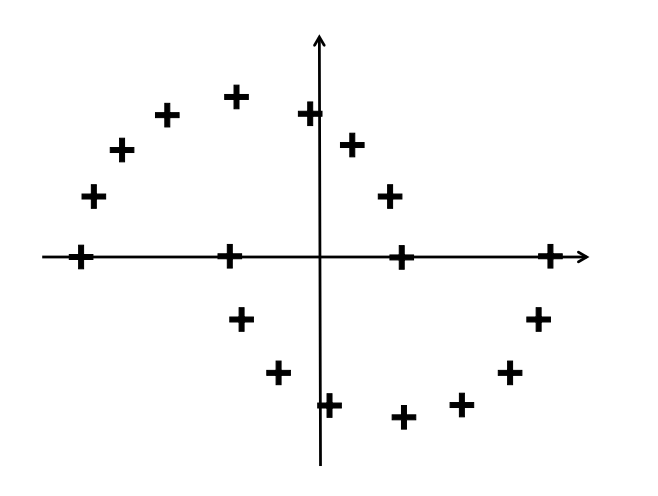
\includegraphics[width=0.5\textwidth,height=0.5\textheight,keepaspectratio]{images/4_28_Jan_2021.png}
 \end{figure}

 \begin{solution}
    \begin{figure}[H]
        \centering
        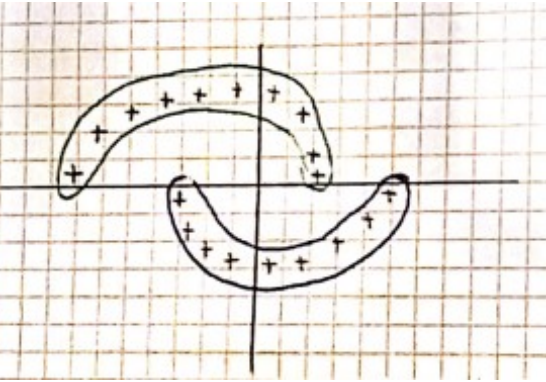
\includegraphics[width=0.5\textwidth,height=0.5\textheight,keepaspectratio]{images/3_4_28_Jan_2021.png}
     \end{figure}
 \end{solution}

 %-----------------------------------------------------------------------------------------------

 \chapter{29 June 2020}

 \begin{figure}[H]
    \centering
    \begin{minipage}{0.45\textwidth}
        
\includegraphics[width=\textwidth,page=3]{images/29_June_2020.pdf}
    \end{minipage}
    \hfill
    \begin{minipage}{0.45\textwidth}
        
\includegraphics[width=\textwidth,page=6]{images/29_June_2020.pdf}
    \end{minipage}
    
    \vspace{1cm}
    
    \centering
    \begin{minipage}{0.45\textwidth}
        
\includegraphics[width=\textwidth,page=9]{images/29_June_2020.pdf}
    \end{minipage}
    \hfill
    \begin{minipage}{0.45\textwidth}
        
\includegraphics[width=\textwidth,page=12]{images/29_June_2020.pdf}
    \end{minipage}
\end{figure}

\clearpage
\section{Exercise 1}
\begin{enumerate}
\item Describe the general framework of binary classification.
    \begin{solution}
        The binary classification problem is a supervised learning problem with:
        
        \begin{itemize}
        \item Domain set $X$ which is the set of all possible objects to make predictions about, where a domain point $\vec{x} \in X$ is called instance and is usually represented by a vector of features
        
        \item Label set $Y = \{-1,+1\}$, that defines the set of all possible labels in this case the labels are only 2
        \end{itemize}
        
        Given a training set $S = ((x_1, y_1) ... (x_m, y_m))$ with $x_i \in X, y_i \in Y$ $\forall i = 1,..,m$ we need to choose an hypothesis class H, which defines the possible models or classification rules, from which we can pick our model to make predictions, and a loss function $l: H \times Z \to \mathbb{R}^+$ where $Z = X \times Y$ that given an hypothesis provides a measure of how much we lose by predicting the value $h(\vec{x})$ for $\vec{x}$ instead of the correct value $y$.
        
        The goal is to find an hypothesis $\hat{h} \in H$ with low generalization error: $L_d(\hat{h}) = E_{z\sim D}[l(\hat{h},z)]$ where:
        
        \begin{itemize}
        \item $D$ is the unknown probability distribution over $Z$ from which $(x_i, y_i) \in S$ have been drawn (as independent samples).
        \end{itemize}
    \end{solution}

\item Discuss the use of the logistic regression model for binary classification and describe how it can be trained using stochastic gradient descent.
\end{enumerate}

\clearpage
\section{Exercise 2}
\begin{enumerate}
\item Introduce the concept of separating hyperplane and describe how it leads to the formulation of hard SVM.
    \begin{solution}
        Given a binary classification problem where:
        \begin{itemize}
        \item Domain set $X$ which is the set of all possible objects to make predictions about, where a domain point $\vec{x} \in X$ is called instance and is usually represented by a vector of features
        \item Label set $Y = \{-1,+1\}$, that defines the set of all possible labels in this case the labels are only 2 
        \item set $S = ((x_1, y_1) ... (x_m, y_m))$ with $x_i \in X, y_i \in Y$ $\forall i = 1,..,m$ is the so called training set
        \end{itemize}
        
        A separating hyperplane is an hyperplane that separates all the points of the training set $S$ into two parts, namely into two halfspaces which contains all and only the points that have either class -1 or +1.
        In case in which the training set $S$ is linearly separable, then there exists more than one such hyperplane and in particular we can define the optimal as the one that maximizes the margin i.e. the distance between the hyperplane and the closest points in $S$ to him.
        
        The optimal separating hyperplane introduced above is exactly the solution computed by the SVM when data are linearly separable. In particular if we define:
        \begin{itemize}
        \item hyperplane as: $L = \{v :\langle \vec{w}, \vec{v} \rangle +b = 0\}$
        \item distance between a point $x$ and $L$: $d(x,L) = \min \{|\vec{x} - \vec{v}|: v \in L\}$
        \end{itemize}
        
        Then the optimal separating hyperplane can be computed as:
        $$\argmax_{(\vec{w},b): \|\vec{w}\|=1 \; i\in\{1,...,m\}} \min |\langle \vec{w},\vec{x}_i \rangle +b| \text{ subject to: } \forall i \; y_i(\langle \vec{w},\vec{x}_i \rangle +b)$$
        
    \end{solution}

\item In most practical situations data are not linearly separable. How can hard SVM be adapted to cope with this situation while still using a linear separation boundary? Formulate this adaptation in the form of an optimization problem, discussing the role and effect of the parameter $\lambda$ that trades the two components of the cost function.
    \begin{solution}
        Soft-SVM is similar to Hard-SVM, but can be used also when training data is not linearly separable (i.e., the training data cannot be perfectly classified with a linear model). Soft-SVM finds a model of large margin while allowing the training set to be inside the margin or wrongly classified. This is obtained by adding slack variables $\xi_i$ to the constraints of hard SVM. The constraint for soft-SVM are then:
        \begin{itemize}
        \item $\xi_i \geq 0$ for each $i = 1,...,m$
        \item $y_i(\langle \vec{w},\vec{x}_i \rangle +b) \geq 1 - \xi_i$ for each $(x_i,y_i)$ $i = 1,...,m$ in the training set where $\vec{w}$ and $b$ defines the model.
        \end{itemize}
        
        The interpretation of $\xi_i$ is the following:
        \begin{itemize}
        \item if $\xi_i = 0$ then $\vec{x}_i$ is correctly classified and outside the margin;
        \item if $0 < \xi_i < 1$ then $\vec{x}_i$ is correctly classified and inside the margin;
        \item if $\xi_i \geq 1$ then $\vec{x}_i$ is wrongly classified.
        \end{itemize}
        
        The function optimized by soft-SVM consider both the margin and the "violation" of the hard-SVM given by $\xi_i$.
        
        Therefore the optimization problem for soft-SVM can be described as follows:
        
        Input: $S = ((\vec{x}_1, y_1) ... (\vec{x}_m, y_m))$ and parameter $\lambda > 0$
        
        Goal: $\min_{\vec{w},b,\vec{\xi}} \lambda\|\vec{w}\|^2 + \frac{1}{m}\sum_{i=1}^m \xi_i$
        
        Output: $\vec{w}, b, \vec{\xi}$
        
        The parameter lambda controls the tradeoff between an high margin with several points misclassified and a small margin with most of the points correctly classified in particular, if $\lambda \approx 0$ then, soft-SVM will produce a model that tries to be as similar as possible as the one produced by hard-SVM namely, it tries to classified as many as possible points correctly. On the other hand, if $\lambda \gg 0$ then, soft-SVM cares almost to maximize the margin therefore, it produces a model that has most of the points misclassified but it has an high margin.
    \end{solution}
\end{enumerate}

\section{Exercise 3}
With reference to the binary classification problem:
\begin{enumerate}
\item Describe how the true error $L_D(h_s)$ of a predictor $h_s$ can be decomposed into approximation $\epsilon_{app}$ and estimation $\epsilon_{est}$ error. Discuss how this decomposition is related to the complexity of the selected hypothesis class and draw a plot with the expected behaviour of the approximation, estimation, and true error, as functions of the complexity of the hypothesis class.
    \begin{solution}
        The generalization error $L_D(h_S)$ can be decomposed into $L_D(h_S) = \epsilon_{app} + \epsilon_{est}$ where $\epsilon_{app} = \min_{h\in H}L_D(h)$ and $\epsilon_{est} = L_D(h_S) - \min_{h\in H}L_D(h)$.
        
        In words:
        \begin{itemize}
        \item $\epsilon_{app}$ = approximation error: is the minimum risk achievable by a predictor in the hypothesis class
        \item $\epsilon_{est}$ = estimation error: is the difference between the approximation error and the error achieved by the ERM predictor
        \end{itemize}
        
        Therefore if we plot in a graph those two error and the $L_D(h_S)$ as functions of the complexity we obtain that:
        \begin{itemize}
        \item $\epsilon_{app}$: will decrease if the complexity decreases if complexity increases
        \item $\epsilon_{est}$: will increase if the complexity increases
        \item $L_D(h_S)$: has a "bell" behaviour
        \end{itemize}
        
        \begin{figure}[H]
        \centering
        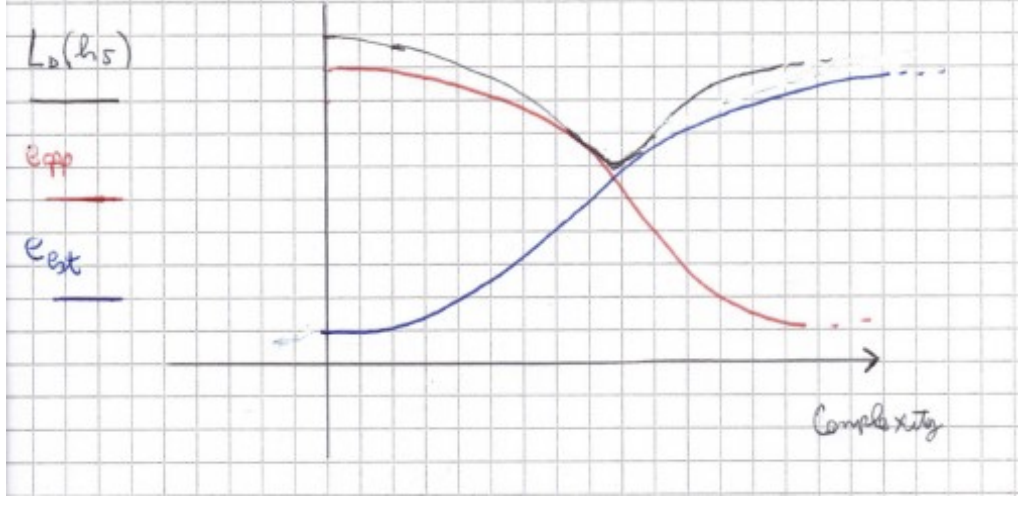
\includegraphics[width=0.6\textwidth]{images/1_3_29_June_2020.png}
        \end{figure}
    
    Notice that a low complexity hypothesis class corresponds to a underfitting situation while a high complexity class corresponds to a overfitting situation.
    \end{solution}
\item Formally introduce the Tikhonov regularization model writing down the function to be optimized. In relation with the previous answer, discuss how Tikhonov regularization can be used to control the fitting-stability trade-off. In particular discuss the behaviour of the approximation, estimation, and true error, as functions of the regularization parameter $\lambda$.
    \begin{figure}[H]
        \centering
        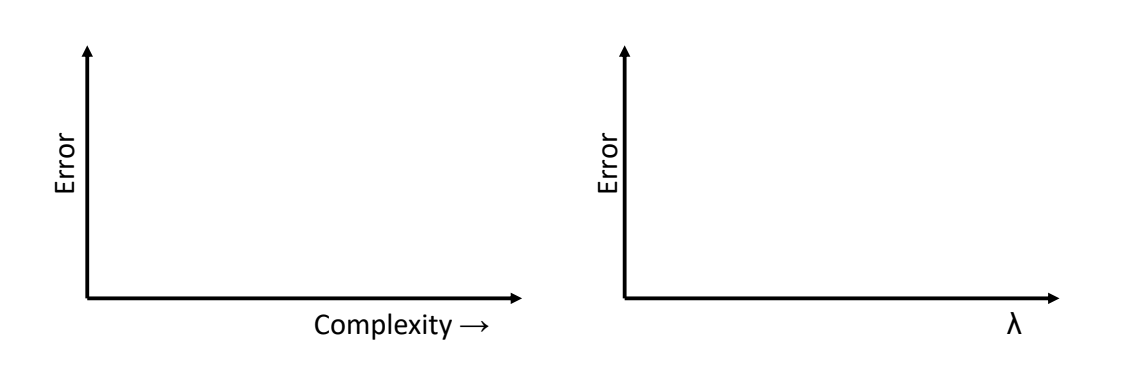
\includegraphics[width=0.6\textwidth,height=0.6\textheight,keepaspectratio]{images/3_29_June_2020.png}
    \end{figure}

    \begin{solution}
        Tikhonov regularization is the Regularized loss minimization paradigm with regularization function $R(\vec{w}) = \lambda\|\vec{w}\|^2$ where $\lambda > 0$ and $\|\vec{w}\|^2$ is the $l_2$ norm of the vector $\vec{w}$.
        
        Therefore the function to be optimized, i.e. minimized is the following: $\argmin_{\vec{w}}(L_S(\vec{w}) + \lambda\|\vec{w}\|^2)$ where $L_S(\vec{w})$ is the training error and $S$ is the training set.
        
        Notice that $\|\vec{w}\|^2$ measures the complexity of the hypothesis $\vec{w}$, while $\lambda$ is the parameter used to tradeoff the empirical risk and the complexity of the model.
        
        Now, the behavior of the $\epsilon_{app}$, $\epsilon_{est}$ and $L_D(h_S)$ in terms of the parameter $\lambda$ is the following:
        \begin{itemize}
        \item $\epsilon_{app}$ will increase if $\lambda$ increases because with a low $\lambda$ we have a complex hypothesis class
        \item $\epsilon_{est}$ will decrease if $\lambda$ increases because with an high $\lambda$ we have a low-complexity hypothesis class
        \item $L_D(h_S)$: has a "bell" behaviour
        \end{itemize}
        
        \begin{figure}[H]
            \centering
            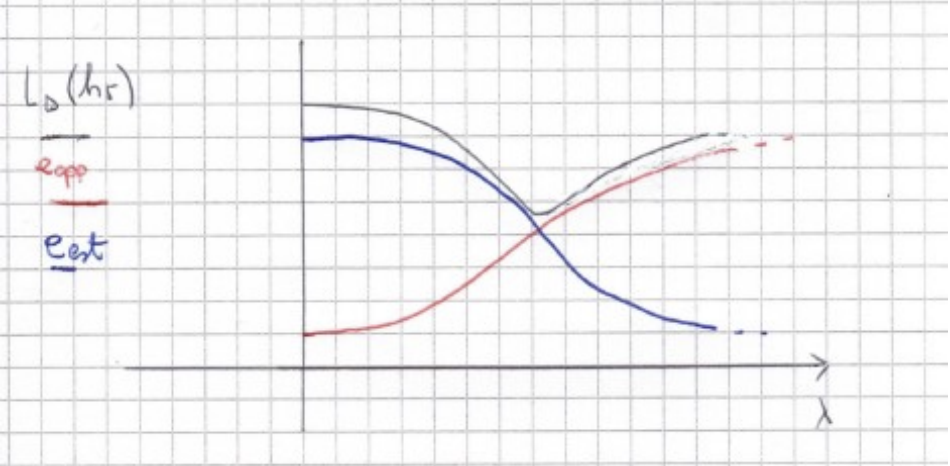
\includegraphics[width=0.6\textwidth]{images/2_3_29_June_2020.png}
            \end{figure}
        \end{solution}
\end{enumerate}


\section{Exercise 4}
\begin{enumerate}
\item Introduce the k-means clustering problem and present the standard (i.e., Lloyd's) algorithm for its solution.
\begin{solution}
    K-means is a cost minimization clustering problem. Let $X' \subseteq X$ be the set of points to be clustered with $X = \{\vec{x}_1,...,\vec{x}_m\}$ while $X'$ is the space of possible points that we assume to be in $\mathbb{R}^d$ (i.e $X' = \mathbb{R}^d$).
    Let $k \in \mathbb{N}^+$ be the number of clusters, that is, with $X$, the input of the problem.
    Let $d(.)$ be a distance function: $d(\vec{x},\vec{x'}) = \|\vec{x} - \vec{x'}\|$.
    
    The goal is to find:
    \begin{itemize}
    \item A partition $C = (C_1,..,C_k)$ of $X$
    \item Centroids $\vec{\mu}_1,...,\vec{\mu}_k$ of $C_1,..,C_k$ respectively
    \end{itemize}
    
    That minimizes the k-means cost function: $\sum_{i=1}^k \sum_{\vec{x}\in C_i} d(\vec{x},\vec{\mu}_i)^2$
    
    To find the solution of this problem we can use an heuristic algorithm called Lloyd's Algorithm. Such algorithm works as follows:
    
    Input: data points $X = \{\vec{x}_1,...,\vec{x}_m\}$ and $k \in \mathbb{N}^+$\\
    Output: $C = (C_1,...,C_k)$ of $X$ and centroids $\vec{\mu}_1,...,\vec{\mu}_k$ of $C_1,...,C_k$ respectively
    
    To produce such things the algorithm works as follows:
    \begin{itemize}
    \item Randomly initialize the centroids $\vec{\mu}_1,...,\vec{\mu}_k$
    \item Until the convergence is not reached iteratively repeats the following steps:
       \begin{enumerate}
       \item Compute each cluster $C_i$ by associating the points to him that closest to its centroids compared to others centroids.
       \item Compute the new centroids for the next iterations.
       \item If the convergence is reached then the output described above will be returned.
       \end{enumerate}
    \end{itemize}
    
    The pseudocode for such algorithm is the following:
    
    \begin{algorithmic}[1]
    \State Randomly choose $\vec{\mu}_1^0,...,\vec{\mu}_k^0$
    \For{t < 0,... do}
       \For{i = 1,...,k}
           \State $C_i \gets \{\vec{x} \in X : i = \argmin_j d(\vec{x},\vec{\mu}_j^t)\}$
       \EndFor
       \For{i = 1,...,k}
           \State $\vec{\mu}_i^{t+1} = \frac{1}{|C_i|}\sum_{\vec{x}\in C_i} \vec{x}$
       \EndFor
       \If{convergence reached}
           \State \Return $C = (C_1,...,C_k), \vec{\mu}_1^{t+1},...,\vec{\mu}_k^{t+1}$
       \EndIf
    \EndFor
    \end{algorithmic}
    
    The convergence criteria that can be used for such algorithm are the following:
    \begin{itemize}
    \item The k-means objective function is no lower than the k-means objective function at the next iteration
    \item $\sum_{i=1}^k d(\vec{\mu}_i^{t+1},\vec{\mu}_i^t) \leq \varepsilon$
    \item $\max_{1\leq i\leq k}d(\vec{\mu}_i^{t+1},\vec{\mu}_i^t) \leq \varepsilon$
    \end{itemize}
    
    Note that if the first criteria is used then, the algorithm will always converge.

    The time complexity is $O(tkmd)$ where $O(kmd)$ is due to the assignments of the points, while $O(md)$ is
    due to the computation of the centroids. Therefore the complexity depends on $t$ which is the number of
    iterations of the algorithm.
    \end{solution}

\clearpage
\item Assume that you need to cluster the points shown in the figure below into $k = 3$ different clusters using k-means. The final solution depends on the initialization of the centroids: suggest two possible initializations, one leading to the optimal solution and one leading to a sub-optimal solution.
\end{enumerate}
\begin{figure}[H]
    \centering
    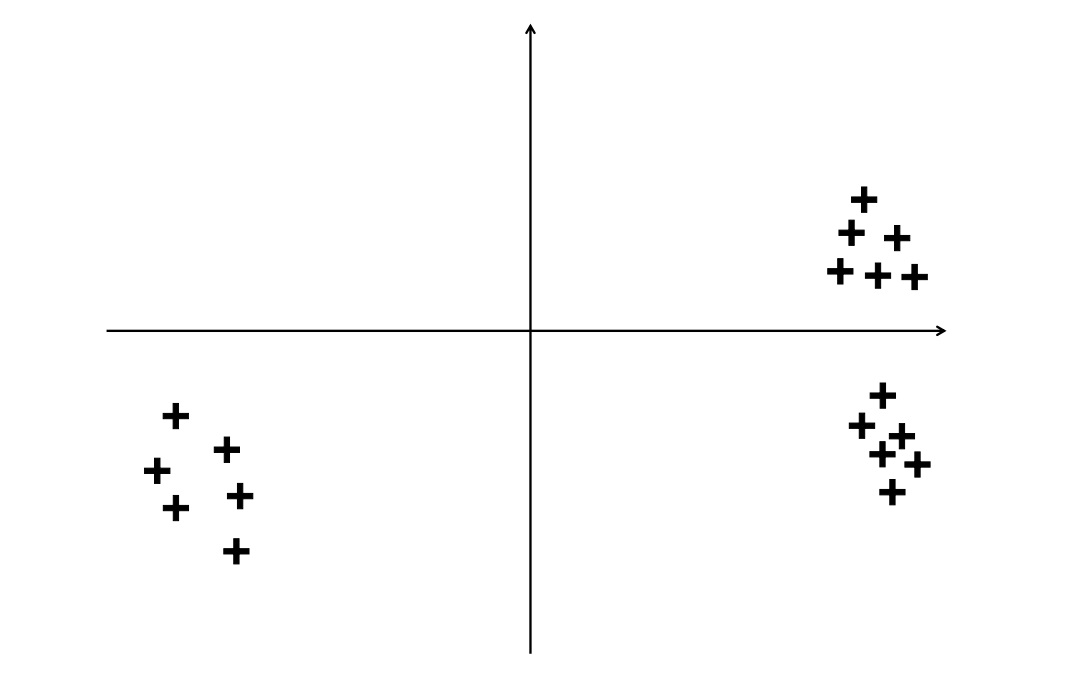
\includegraphics[width=0.6\textwidth,height=0.6\textheight,keepaspectratio]{images/4_29_June_2020.png}
 \end{figure}

    \begin{solution}
        \begin{figure}[H]
        \centering
        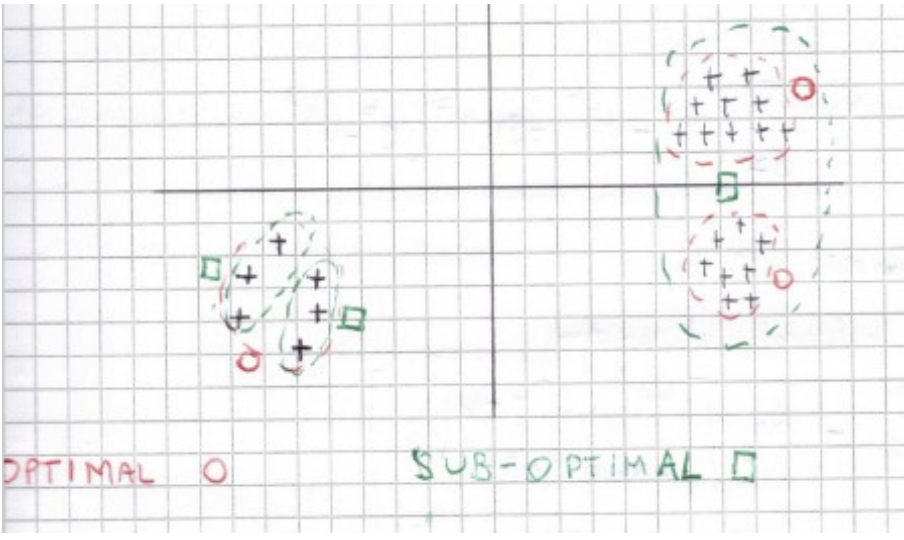
\includegraphics[width=0.9\textwidth]{images/2_4_29_June_2020.png}
        \end{figure}
    \end{solution}

%-----------------------------------------------------------------------------------------------

\chapter{21 February 2020}

\begin{figure}[H]
    \centering
    \begin{minipage}{0.45\textwidth}
        
\includegraphics[width=\textwidth,page=1]{images/21_Feb_2020.pdf}
    \end{minipage}
    \hfill
    \begin{minipage}{0.45\textwidth}
        
\includegraphics[width=\textwidth,page=2]{images/21_Feb_2020.pdf}
    \end{minipage}
    
    \vspace{1cm}
    
    \centering
    \begin{minipage}{0.45\textwidth}
        
\includegraphics[width=\textwidth,page=3]{images/21_Feb_2020.pdf}
    \end{minipage}
    \hfill
    \begin{minipage}{0.45\textwidth}
        
\includegraphics[width=\textwidth,page=4]{images/21_Feb_2020.pdf}
    \end{minipage}
\end{figure}
\section{Exercise 1}
\begin{enumerate}
\item Provide the formulation of PAC learning (including the definition of loss, risk, training algorithms, etc.).
    \begin{solution}        
        An hypothesis class H is PAC (Probably Approximately Correct) learnable with respect 
        to Z and a loss function $l: H\times Z \to \mathbb{R}^+$, if there exists a function $m_H: 
        (0,1)^2 \to \mathbb{N}$ (sample complexity) and a learning algorithm such that for 
        every $\delta \in (0,1)$, $\varepsilon \in (0,1)$, for every distribution D over Z and for 
        every true labeling function $f: X \to \{0,1\}$, if the realizability assumption holds with 
        respect to H, D, f; when running the learning algorithm on $m \geq m_H(\varepsilon, 
        \delta)$ iid samples generated by D and labeled by f the algorithm returns an 
        hypothesis h such that, with probability $\geq 1-\delta$: $L_{D,f}(h) \leq \varepsilon$.
        
        Where:
        \begin{itemize}
        \item $l: H\times Z \to \mathbb{R}^+$ where $Z = X\times Y$ is the loss function namely a 
        function that given an hypothesis provides a measure of how much we lose by 
        predicting the value $h(\vec{x})$ for $\vec{x}$ instead of the correct value.
        
        \item A learning algorithm is a type of algorithm that given input data it learns a function 
        that maps the input into output also for data it has not seen yet.
        
        \item $L_{D,f}(h) = E_{z\sim D}[l(h,z)]$ is the so called risk or generalization error.
        \end{itemize}
    \end{solution}
\clearpage
\item In the context of PAC learning define the concept of realizability and discuss how the formulation above changes when the realizability assumption cannot be made.
    \begin{solution}
        
        The realizability assumption is the assumption that consists of having an hypothesis 
        $h^* \in H$ such that $L_{D,f}(h^*) = 0$. If this assumption doesn't hold, then the 
        formulation of PAC learning changes into agnostic PAC learning.
        
        An hypothesis class H is agnostic PAC learnable with respect to Z and a loss function $l: 
        H\times Z \to \mathbb{R}^+$, if there exists a function $m_H: (0,1)^2 \to \mathbb{N}$ 
        (sample complexity) and a learning algorithm such that for every $\delta \in (0,1)$, 
        $\varepsilon \in (0,1)$, for every distribution D over Z, when running the learning 
        algorithm on $m \geq m_H(\varepsilon, \delta)$ iid samples generated by D the 
        algorithm returns an hypothesis such that, with probability $\geq 1-\delta$: $L_{D,f}(h) 
        \leq \min_{h'\in H} L_{D,f}(h') + \varepsilon$ where $L_{D,f}(h) = E_{z\sim D}[l(h,z)]$.
        \end{solution}
\item Provide a (probabilistic) bound on the generalization error for the ERM when working with finite hypothesis classes (proof not needed).
    \begin{solution}        
        Let H be a finite hypothesis class. Let $\delta \in (0,1)$, $\varepsilon \in (0,1)$, $m \in 
        \mathbb{N}$ such that: $m \geq \frac{\log(|H|/\delta)}{\varepsilon}$, then for any 
        labeling function f, for any distribution D for which the realizability assumption holds 
        with probability $\geq 1-\delta$ we have that for every ERM hypothesis $h_S$ it holds 
        that: $L_{D,f}(h_S) \leq \varepsilon$.
    \end{solution}
\end{enumerate}

\clearpage
\section{Exercise 2}
\begin{enumerate}
\item Introduce the neural network model highlighting its main components and pointing out which are the parameters to be learned in the training process. Describe how the output layer of a neural network for binary classification can be designed.
    \begin{solution}        
        Neural networks models are the most complex models that we can use. To use them we need to define the architecture of a neural network i.e. the graph specifics or practically speaking the number of edges and neurons of a neural network and the activation function.
        
        Therefore the hypothesis class of neural networks becomes:
        $$H_{V,E,\sigma} = \{h_{V,E,\sigma,w}: \mathbb{R}^{|V_0|-1} \to \mathbb{R}^{|V_T|} \text{ where w is a mapping from E to R}\}$$
        So, the learning process of a neural network is aimed to learn the weights in order to define a function that maps the set of edges to the set of real numbers.
        
           \begin{itemize}
        \item Layers are not fully connected one's like for MLP. That means given a non fully connected layer of a CNN we have that the neurons of the next layer are connected with not all the neurons of the current one
        
        \item Parameters are shared in a layer. In addition to what we have said before, namely that the layers are not fully connected, the weights on such edges are the same for a certain subset of edges therefore, the numbers of parameter to learn decreases
        \end{itemize}
     In particular, about the graph
 specific, one important thing is that the output layer of the neural network must be composed by only two neurons for binary classification one used to highlighting the probability that the label of the input will be +1 while the other to highlighting the probability that the label of the input will be -1. This is due to the fact that, binary classification is a problem that has only two possible output values i.e. the values +1 or -1. For what concerns the other layers and the activation function, a good strategy to choose them, is to copy the architecture of neural networks already used in literature that works well with the problem of binary classification.
        
        One neuron?
    \end{solution}
\clearpage
\item Consider a fully connected neural network $N$ with $L = 4$ layers, with $n_1 = 5$ neurons in the input layer, $n_2 = n_3 = 4$ neurons in the two inner layers and a single neuron ($n_4 = 1$) in the last (i.e., output) layer. How many trainable parameters are there in the network? How is this number related to the number of neurons in each layer?
    \begin{solution}
        \# of trainable parameters: $\left(n_1 + 1\right)\left(n_2\right) + \left(n_2 + 1\right)n_3 + \left(n_3 + 1\right)n_4$

        \begin{align*}
        &= 6 \cdot 4 + 5 \cdot 4 + 5 \cdot 1 \\
        &= 24 + 20 + 5 = 49
        \end{align*}
    \end{solution}

\item Which provisions are used in the Convolutional Neural Network (CNN) model to reduce the number of trainable parameters? Highlight in your answer the differences with respect to the fully connected model.
    \begin{solution}        
        The main provision done by CNN to reduce the number of parameters are the followings:
        
        \begin{itemize}
        \item Layers are not fully connected one's like for MLP. That means given a non fully connected layer of a CNN we have that the neurons of the next layer are connected with not all the neurons of the current one
        
        \item Parameters are shared in a layer. In addition to what we have said before, namely that the layers are not fully connected, the weights on such edges are the same for a certain subset of edges therefore, the numbers of parameter to learn decreases
        \end{itemize}
    \end{solution}
\end{enumerate}

\clearpage
\section{Exercise 3}
With reference to the binary classification problem:
\begin{enumerate}
\item Describe a framework under which the decision boundary can be an arbitrary polynomial function of degree $M$.
    \begin{solution}
        To have decision boundaries that are polynomial functions of degree M we can use two strategies:
        
        \begin{itemize}
        \item We can use SVM with polynomial kernels with Q=M
        
        \item We can use different representation of the data namely feature expansion/transformation where we map a vector $\vec{x}$ to a polynomial function of degree M in the features $x_i's$ of $\vec{x}$ and then use linear models with the new feature space.
        
        Ex $\vec{x} \in R \to \varphi(\vec{x}) = \begin{bmatrix}
        x_1 \\
        . \\
        . \\
        x_M
        \end{bmatrix} \to \text{ linear model for the transoformed } \\ \varphi(\vec{x}) = w_0+w_1x_1 + \cdots + w_Mx_M \text{ and so for binary classification } \\ sign(w_0+w_1x_1 + \cdots + w_Mx_M)$
        \end{itemize}
    \end{solution}
\item Discuss how this can be related to kernel SVM, possibly highlighting which is the advantage of the "kernel" interpretation.
    \begin{solution}
        What we have introduced in the previous point is related to Kernels SVM because to have polynomial functions as boundaries we use polynomial kernels with Q=M. In addition to that the main advantage is that we do not have to apply any transformation of the input because everything is done by the kernel.
    \end{solution}
\clearpage
\item Assuming one has $(x_i, y_i), i \in [m]$ data points with $m$ "small", describe a procedure to perform the selection of $M$ (deciding the "most suitable" degree of the polynomial boundary), $M \in \{2, 3, 4, .., 10\}$.
    \begin{solution}
        The strategy to select the best value for parameter M is to use cross-validation and once M is chosen we use all the data to learn the best model with such parameter.
        
        To be more precise, cross validation consists in a way to select a value of a parameter $\vartheta$ by understanding what is the best value that such parameter can assume with the data we have.
        To do so, we split the dataset into k different folds of size m/k (this quantity is supposed to be integer). Then for each value of the parameter $\vartheta$ we find the best model for all the possible k-1 folds that we can select. In addition to that, we compute the average error of each parameter as the average of the errors on the folds left out, and when we have repeated such procedure for all the values of the parameters, then we select the optimal one by choosing the one that minimizes the error computed for each parameter. To conclude, we train our model on all the dataset with the parameter found.
        
        The pseudo code is the following:
        \begin{algorithmic}[1]
            \State Input: $S = ((\bar{x}_1, y_1) \ldots (\bar{x}_m, y_m))$; set of parameters $\theta$; integer $k$; learning algorithm $A$
            
            \State Split $S$ into $S_1, \ldots, S_k$
            
            \For{$\theta \in \Theta$}
                \For{$i = 1 \ldots k$}
                    \State $h_{i,\theta} = A(S\setminus S_i; \theta)$
                    \State $error(\theta) = \frac{1}{k}\sum_{i=1}^k L_{S_i}(h_{i,\theta})$
                \EndFor
            \EndFor
            
            \State Output: $\theta^* = \argmin_\theta(error(\theta))$
            \State $h_{\theta^*} = A(S; \theta^*)$
        \end{algorithmic}
    \end{solution}
\end{enumerate}

\clearpage
\section{Exercise 4}
\begin{enumerate}
\item Introduce the problem of dimensionality reduction, describing what is the input, what is the output, and what is its goal.

\item Consider a linear regression problem with squared loss, where the input feature vectors are $\mathbf{x}_1, \mathbf{x}_2, \ldots, \mathbf{x}_m$. Assume that the (design) matrix $\mathbf{X}$, whose $i$-th row is $\mathbf{x}_i^T$ is such that $\mathbf{X}^T\mathbf{X}$ is almost singular. (Remember that a square matrix is singular if and only if it is not invertible.) Explain how dimensionality reduction can be used to reduce the number of parameters to be estimated and to learn a model in this situation.

\item Consider the two datasets with points $\mathbf{x} \in \mathbb{R}^2$ shown in Figure (a) and (b) below. For both datasets, describe i) whether it is possible to meaningfully reduce the dimensionality of the data and ii) what is the most appropriate dimension of the data after dimensionality reduction.
    \begin{figure}[H]
        \centering
        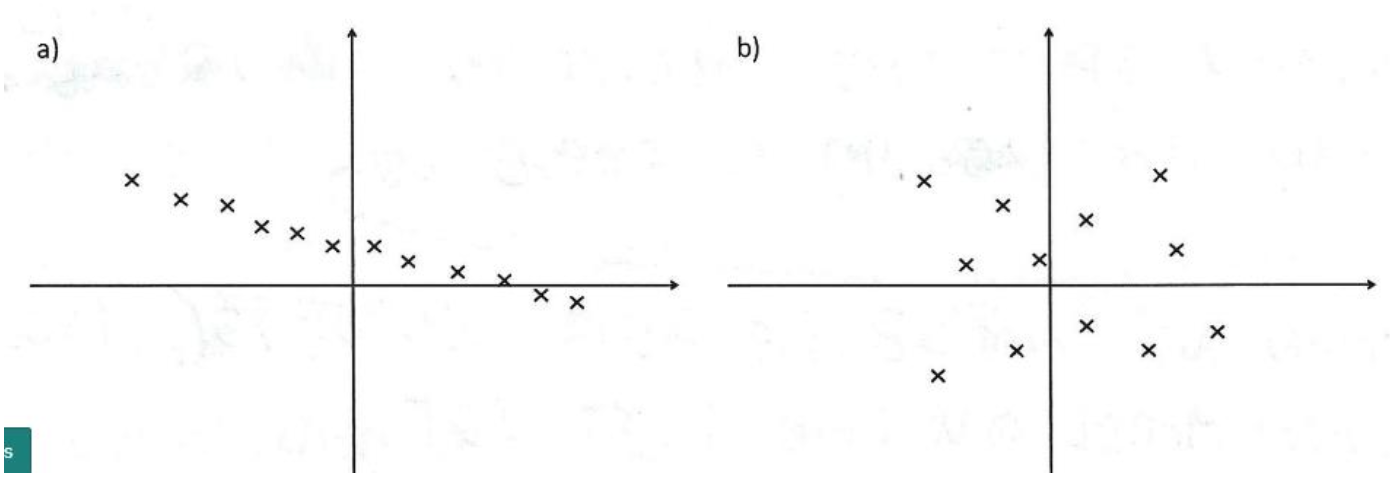
\includegraphics[width=0.7\textwidth,height=0.7\textheight,keepaspectratio]{images/4_21_Feb_2020.png}
    \end{figure}
\end{enumerate}

%-----------------------------------------------------------------------------------------------

\chapter{7 February 2020}

\begin{figure}[H]
    \centering
    \begin{minipage}{0.45\textwidth}
        \includegraphics[width=\textwidth,page=3]{images/ex1_7_Feb_2020.png}
    \end{minipage}
    \hfill
    \begin{minipage}{0.45\textwidth}
        \includegraphics[width=\textwidth,page=6]{images/ex2_7_Feb_2020.png}
    \end{minipage}
    
    \vspace{1cm}
    
    \centering
    \begin{minipage}{0.45\textwidth}
        \includegraphics[width=\textwidth,page=8]{images/ex3_7_Feb_2020.png}
    \end{minipage}
    \hfill
    \begin{minipage}{0.45\textwidth}
        \includegraphics[width=\textwidth,page=11]{images/ex4_7_Feb_2020.png}
    \end{minipage}
\end{figure}

\clearpage
\section{Exercise 1}
Consider the regression problem when the training data is \( S = \{(x_1, y_1), (x_2, y_2), \ldots (x_m, y_m)\} \) with \( x_i = [x_{i,1}, x_{i,2}] \in \mathbb{R}^2 \) and \( y_i \in \mathbb{R} \) for \( i = 1, \ldots, m \).

\begin{enumerate}
    \item Formally define the problem when the hypothesis class is \( \mathcal{H} = \{h(x) \text{ s.t. } h(x) = w_0 + w_1 x_1 + w_2 x_2; w_0, w_1, w_2 \in \mathbb{R}\} \) and the squared loss is used. In particular, describe what the goal is.
        \begin{solution}
            Given the training data \( S = \{ (x_1, y_1), \ldots, (x_m, y_m) \} \), with \( x_i \in \mathbb{R}^2 \), \( y_i \in \mathbb{R} \) for \( i = 1, \ldots, m \), our goal is to find a hypothesis \( \hat{h} \) that minimizes the generalization error. That is, we want to find \( \hat{h} \) such that  
            \[
            E_{(x, y) \sim D} [\ell(\hat{h}, (x, y))]
            \]
            is minimized, where  
            \[
            \ell(\hat{h}, (x, y)) = (\hat{h}(x) - y)^2
            \]
            and \( D \) is the (unknown) probability distribution from which \( (x_i, y_i) \in S \), \( i = 1, \ldots, m \) have been drawn independently.
        \end{solution}
    \clearpage
    \item Describe \( \ell_2 \) regularization within the context described above. Given an hypothesis \( h \in \mathcal{H} \), let \( L_S(h) \) be its training error (i.e., the average loss on the training set), \( J(h) = L_S(h) + \lambda R(h) \) be the regularized training error, where \( R(h) \) is the \( \ell_2 \) regularization function. Formally define the regularization function for \( \ell_2 \) regularization and \textit{derive} the hypothesis that minimizes the \( \ell_2 \) regularized training error.
        \begin{solution}
            \( l_1 \) regularization in the context above corresponds to ridge regression. In particular, the design matrix is  
            \[
            X = \begin{bmatrix} 
            -\bar{X}_1^1 \\ 
            -\bar{X}_2^1 \\ 
            -\bar{X}_3^1 
            \end{bmatrix}, 
            \text{ where } \bar{X}_i^1 = [1, x_{i_1}, x_{i_2}] \text{ and } \bar{Y} = \begin{bmatrix} 
            Y_1 \\ 
            Y_2 \\ 
            \vdots \\ 
            Y_n 
            \end{bmatrix}. 
            \]  
        
            Let \( \vec{w} = \begin{bmatrix} 
            w_0 \\ 
            w_1 \\ 
            w_2 
            \end{bmatrix} \). Since an hypothesis block is defined by the coefficient vector \( \vec{w} \), we have that the training error is  
            \[
            L_s(\hat{h}) = L_s(\vec{w}) = \frac{1}{m} \left( \vec{Y} - X \vec{w} \right)^T \left( \vec{Y} - X \vec{w} \right), 
            \]  
            and minimizing \( L_s(\hat{h}) \) (or \( L_s(\vec{w}) \)) corresponds to minimizing  
            \[
            \left( \vec{Y} - X \vec{w} \right)^T \left( \vec{Y} - X \vec{w} \right), 
            \]  
            In ridge regression, the regularization function \( R(\hat{h}) = \| \vec{w} \|^2 \), therefore, the hypothesis that minimizes the regularized training error \( L_s(\hat{h}) + \lambda R(\hat{h}) \) is  
            \[
            \arg \min_{\vec{w}} \left( \left( \vec{Y} - X \vec{w} \right)^T \left( \vec{Y} - X \vec{w} \right) + \lambda \vec{w}^T \vec{w} \right).
            \]  
            To find \( \vec{w} \), we compute the gradient and set it to zero:  
            \[
            \frac{\partial (L_s(\vec{w}) + \lambda R(\vec{w}))}{\partial \vec{w}} = 2 \lambda \vec{w} - 2 X^T \left( \vec{y} - X \vec{w} \right) = 0.
            \]  
            This leads to the equation:  
            \[
            (\lambda I + X^T X) \vec{w} = X^T \vec{y} \Leftrightarrow \vec{w} = (\lambda I + X^T X)^{-1} X^T \vec{y}.
            \]  
            Note that \( \lambda I + X^T X \) is positive definite, thus invertible.
        \end{solution}
    \item Given an hypothesis \( h \), let \( \mathcal{L}(h) \) be the true (or generalization) error of \( h \). Let \( h_s \) be the hypothesis that, given data \( S \), minimizes the regularized training error \( J(h) \). Plot the typical behavior of \( L_S(h_s) \) and \( \mathcal{L}(h_s) \) as a function of \( \lambda \geq 0 \), and describe how this is linked to overfitting.
        \begin{solution}
            \begin{tikzpicture}[scale=1.2]
                % Axes
                \draw[->] (0,0) -- (5,0) node[right] {$\lambda$};
                \draw[->] (0,0) -- (0,4) node[left] {$L_D(\vec{w})$};
                
                % Labels on y-axis
                \node[left] at (0,0.8) {$L_S(h_S)$};
                \node[left] at (0,2) {$L_D(h_S)$};
                
                % Curves
                % Training error curve (dashed) - keeping it below the main curve
                \draw[dashed] (0,0.8) .. controls (1.5,0.9) and (3,1.8) .. (4.8,2.8);
                
                % Generalization error curve (solid) - starting from L_D(h_S)
                \draw[thick] (0,2) .. controls (1,1.6) and (2.5,1.8) .. (4.8,3);
                
                % Top horizontal dashed line
                \draw[dashed] (0,3.5) -- (4.8,3.5);
            \end{tikzpicture}

            For low values of $\lambda$ we are ignoring the complexity of $h_S$ and only care about minimizing the training error, thus we may find $h_S$ with low training error $L_S(h_S)$ but high generalization error $L_D(h_S)$, which corresponds to overfitting. Increasing $\lambda$ we take the complexity of $h_S$ more and more into account, and for some value of $\lambda$ we may have a good balance between training error and complexity, thus providing an hypothesis $h_S$ with lower generalization error.
        \end{solution}
\end{enumerate}

\clearpage
\section{Exercise 2}
Consider the classification problem in machine learning.

\begin{enumerate}
    \item Provide a formal definition, describing data, loss functions, classification rules etc.
        \begin{solution}
            The classification problem is a supervised learning problem, with:
            \begin{itemize}
            \item domain set X, that is the set of all possible objects to make predictions about, where a domain point $\vec{x} \in X$ is called instance, and is usually represented by a vector of features
            
            \item label set Y, that defines the set of possible labels. Y is a discrete set in classification. For example, in binary classification Y = \{-1,1\} or similar
            \end{itemize}
            
            Given training data $S = ((\vec{x}_1, y_1), ..., (\vec{x}_m, y_m))$, with $\vec{x}_i \in X$, $y_i \in Y$ $\forall i=1,...,m$, we need to choose an hypothesis class H, which defines the possible models or classification rules we can pick to make prediction, and a loss function $l: H \times Z \to \mathbb{R}^+$, with $Z = X \times Y$, that given an hypothesis provides a measure of how much we lose by predicting the label $h(\vec{x})$ for $\vec{x}$ instead of the (correct) label y. The goal is then to find an hypothesis $h \in H$ with low generalization error, defined as:
            
            $L_D(h) = E_{z\sim D}[l(h,z)]$
            
            where D is the unknown probability distribution over Z from which $(\vec{x}_i, y_i) \in S$, $i=1,...,m$, have been drawn (as independent samples).
        \end{solution}

    \item Assuming inputs (or features) \( x \in \mathbb{R} \), and consider the model class, which is a modified version of logistic regression, defined as the set of models obtained composing the sigmoid function  
    \[
    \frac{1}{1 + e^{-z}}
    \]
    with the function  
    \[
    z = h_w(x) = w_1 + w_2x^2
    \]
    where the parameters are \(\mathbf{w} = [w_1, w_2]^\top \in \mathbb{R}^2\). Assume the loss is \(\ell(h, (x_i, y_i)) = (y_i - h(x_i))\) if \(y_i = 1\), and \(\ell(h, (x_i, y_i)) = h(x_i)\) if \(y_i = 0\). Write the stochastic gradient descent update for learning this model from data \((x_i, y_i)\), \(i = 1, ..., m\).
        \begin{solution}
            In general, for stochastic gradient descent (SGD), let $\vec{w}^{(t)}$ be the weights defining the model in iteration t. Then the update rule is given by:
            
            \begin{itemize}
            \item pick $(\vec{x}_i, y_i) \in S$ uniformly at random
            \item $\vec{w}^{(t+1)} \leftarrow \vec{w}^{(t)} - \eta \nabla l(\vec{w}^{(t)}, (\vec{x}_i,y_i))$
            \end{itemize}
            
            We need to compute $\nabla l(\vec{w}^{(t)}, (\vec{x}_i,y_i))$ for specific model class and loss we are considering. Each model h in our model class is a function of the form:
            $$h(x) = \frac{1}{1+e^{-(w_1+w_2x^2)}}$$
            Since the loss depends on the value of $y_i$, the gradient will depend on $y_i$ as well.
            
            Let's consider the two cases:
            
            i) $y_i = 1 \Rightarrow \nabla l(h(x),(x,y)) = \left[\frac{\partial l}{\partial w_1}, \frac{\partial l}{\partial w_2}\right]^T$, and:
            
            $\frac{\partial l}{\partial w_1} = \frac{\partial z}{\partial w_1} \cdot \frac{\partial l}{\partial z} = 1 \cdot \frac{\partial}{\partial z}(1-\frac{1}{1+e^z}) = -\frac{e^z}{(1+e^z)^2}$, with $z=w_1+w_2x^2$
            
            $\frac{\partial l}{\partial w_2} = \frac{\partial z}{\partial w_2} \cdot \frac{\partial l}{\partial z} = x^2 \cdot (-\frac{e^z}{(1+e^z)^2}) = -x^2\frac{e^z}{(1+e^z)^2}$
            
            ii) $y_i = 0 \Rightarrow \nabla l(h(x),(x,y)) = \left[\frac{\partial l}{\partial w_1}, \frac{\partial l}{\partial w_2}\right]^T$, and:
            
            $\frac{\partial l}{\partial w_1} = \frac{\partial z}{\partial w_1} \cdot \frac{\partial l}{\partial z} = 1 \cdot \frac{\partial}{\partial z}(\frac{1}{1+e^z}) = \frac{e^z}{(1+e^z)^2}$
            
            $\frac{\partial l}{\partial w_2} = \frac{\partial z}{\partial w_2} \cdot \frac{\partial l}{\partial z} = x^2\frac{e^z}{(1+e^z)^2}$
            
            Therefore the SGD update rule is:
            \begin{itemize}
            \item pick $(\vec{x}_i,y_i) \in S$ uniformly at random;
            \item $z \leftarrow w_1^{(t)}+w_2^{(t)}x_i^2$
            \item if $y_i=1$ then $\vec{w}^{(t+1)} \leftarrow \vec{w}^{(t)} + \eta\begin{bmatrix} e^z/(1+e^z)^2 \\ x^2e^z/(1+e^z)^2 \end{bmatrix}$
            \item else $\vec{w}^{(t+1)} \leftarrow \vec{w}^{(t)} - \eta\begin{bmatrix} e^z/(1+e^z)^2 \\ x^2e^z/(1+e^z)^2 \end{bmatrix}$
            \end{itemize}
        \end{solution}
\end{enumerate}

\section{Exercise 3}
The Soft-SVM classifier aims at minimizing the following function:  
\[
\lambda||\mathbf{w}||^2 + \frac{1}{m}\sum_i \xi_i.
\]

\begin{enumerate}
    \item Briefly explain how the Soft-SVM classification method works and which are the constraints under which the function has to be minimized.
        \begin{solution}
            Soft-SVM is similar to hard-SVM, but can be used also when the training data is not linearly separable, (i.e., the training data cannot be perfectly classified with a linear model). Soft-SVM finds a model of large margin while allowing some points of the training set to be inside the margin or wrongly classified. This is obtained by adding slack variables $\xi_i$ to the constraints of hard-SVM. The constraints for soft-SVM are then:
            \begin{itemize}
            \item $\xi_i \geq 0$ for each $i=1,...,m$
            \item $y_i(\langle \vec{w}, \vec{x}_i \rangle +b) \geq 1-\xi_i$ for each point $(\vec{x}_i, y_i)$, $i=1,...,m$ in the training set, where $\vec{w}$ and b define the model. 
            \end{itemize}
            The interpretation of $\xi_i$ is the following: if $\xi_i=0$, then $\vec{x}_i$ is correctly classified and outside the margin; if $0<\xi_i<1$, then $\vec{x}_i$ is correctly classified but inside the margin. If $\xi_i \geq 1$ then $\vec{x}_i$ is incorrectly classified. The function optimized by soft-SVM considers both the margin and the "violation" of the hard-SVM given by $\xi_i$.
        \end{solution}

    \item The figure shows the results of a binary classification performed using a Soft-SVM model with parameter \(\lambda = 1\). The training samples are the circles and diamonds and the two shapes correspond to the two classes to which the samples belong. The solid line is the computed separating hyperplane, while the dotted lines represent the margins. For which points \(\xi_i\) is different from 0?
        \begin{solution}
            See the points circled in blue in the figure. Since they are not correctly classified, the corresponding $\xi_i's$ are > 0.
        \end{solution}
    
    \clearpage
    \item Does the margin increase or decrease when \(\lambda\) decreases? Guess how the solution changes when a very small value for the \(\lambda\) parameter (i.e., \(\lambda \approx 0\)) is used, and draw an estimate of the separating hyperplane that could be obtained in this case.
        \begin{figure}[H]
            \centering
            \includegraphics[width=0.6\textwidth,height=0.6\textheight,keepaspectratio]{images/3_7_Feb_2020.png}
        \end{figure}
        \begin{solution}
            When $\lambda$ decreases, the term $\frac{1}{m}\sum_{i=1}^m \xi_i$ becomes more important in the function minimized by soft-SVM, therefore a model that reduces the values of $\xi_i's$ is sought, even if the margin is smaller. In particular, for the dataset shown in the figure, when $\lambda \approx 0$ the margin is very small, since there is a linear model (shown in green in the figure) of small margin but that correctly classifies all points in the training set, so that $\xi_i=0$ $\forall i=1,...,m$.
        \end{solution}
\end{enumerate}

\section{Exercise 4}
\begin{enumerate}
    \item Briefly introduce the clustering problem.
        \begin{solution}
            Clustering is the problem of grouping a set of objects such that similar objects end up in the same group and dissimilar objects are separated into different groups.
            
            More formally, the problem has the following input and output:
            
            Input: set X of objects and a distance function $d: X \times X \to \mathbb{R}^+$
            
            Output: a partition of X into clusters, that is $C = (C_1, C_2, ..., C_k)$ such that:
            \begin{itemize}
            \item $\bigcup_{i=1}^k C_i = X$
            \item for all $i \neq j : C_i \cap C_j = \emptyset$
            \end{itemize}
            
            (Sometimes the input includes the number k of clusters.)
            
            The partition to be produced in output depends on the specific definition of the problem, and is sometimes captured by defining a cost for a given clustering.
        \end{solution}

    \item Define and explain the cost function used in K-means clustering.
        \begin{solution}
            Let the input data points be $\vec{x}_1, \vec{x}_2, ..., \vec{x}_m$ with $\vec{x}_i \in \mathbb{R}^d$ for $i=1,...,m$. The k-means cost function is:
            
            $$\sum_{i=1}^k \sum_{\vec{x}\in C_i} d(\vec{x},\vec{\mu}_i)^2$$
            
            where $C_1,...,C_k$ are the clusters, $d(\cdot,\cdot)$ is the Euclidean distance in $\mathbb{R}^d$, and $\vec{\mu}_i$ is the center of cluster $C_i$ for $i=1,...,k$ (the centers are part of the output). Therefore, the cost of a clustering for k-means is defined as the sum of the squares of the distances of each point to the center of the cluster it belongs to.
        \end{solution}
    \item Consider the data in the figure below where each point \( x \in \mathbb{R}^2 \) is represented by a cross. Show the results (i.e., draw approximately the final centroid locations and the final assignment of the points to the clusters) of clustering into \( k = 2 \) clusters with K-means when  
        \begin{itemize}
            \item (a) the initial centers for the algorithm are the circles;  
            \item (b) the initial centers for the algorithm are the squares.  
        \end{itemize}
        Is one solution \textit{significantly} better than the other one? Briefly motivate your answer.
        \begin{figure}[H]
            \centering
            \includegraphics[width=0.6\textwidth,height=0.6\textheight,keepaspectratio]{images/4_7_Feb_2020.png}
        \end{figure}
        \begin{solution}
            The solutions are shown in the figure. There is no solution that is significantly better than the other one, since the data consists of 4 groups of points that are essentially symmetric with respect to the origin, and the 2 solutions are just 2 different ways to group them into 2 groups. Also, the silhouette coefficient of the 2 solutions is probably very similar.
            \begin{figure}[H]
                \centering
                \includegraphics[width=0.9\textwidth,height=0.6\textheight,keepaspectratio]{images/3_4_7_Feb_2020.png}
            \end{figure}
        \end{solution}
\end{enumerate}

%-----------------------------------------------------------------------------------------------

\chapter{4 September 2019}

\begin{figure}[H]
    \centering
    \begin{minipage}{0.45\textwidth}
        \includegraphics[width=\textwidth,page=3]{images/4_Sept_2019.pdf}
    \end{minipage}
    \hfill
    \begin{minipage}{0.45\textwidth}
        \includegraphics[width=\textwidth,page=6]{images/4_Sept_2019.pdf}
    \end{minipage}
    
    \vspace{1cm}
    
    \centering
    \begin{minipage}{0.45\textwidth}
        \includegraphics[width=\textwidth,page=9]{images/4_Sept_2019.pdf}
    \end{minipage}
    \hfill
    \begin{minipage}{0.45\textwidth}
        \includegraphics[width=\textwidth,page=12]{images/4_Sept_2019.pdf}
    \end{minipage}
\end{figure}

\clearpage
\section{Exercise 1}
Consider the binary classification problem:

\begin{enumerate}
\item With reference to the binary classification problem, introduce the concepts of model class, loss function, empirical risk and (expected) risk.
    \begin{solution}
        The binary classification problem is a supervised learning problem with:
        \begin{itemize}
        \item Domain set X which is the set of all possible objects to make predictions about, where a domain point $\vec{x} \in X$ is called instance and is usually represented by a vector of features
        
        \item Label set $Y = \{-1,+1\}$, that defines the set of all possible labels in this case the labels are only 2
        
        \item Model class H: is the set of functions that represents a mapping from X to Y
        
        \item Loss function: is a function $l: H\times Z \to \mathbb{R}^+$ where $Z = X\times Y$ that, given an hypothesis provides a measure of how much we lose by predicting the value $h(\vec{x})$ for $\vec{x}$ instead of the correct value y
        
        \item Generalization error: $L_d(h) = E_{z\sim D}[l(h,z)]$ where D is the unknown probability distribution over Z from which $(x_i,y_i) \in S$ have been drawn (as independent samples)
        
        \item Training error: $L_S(h) = \frac{1}{m}\sum_{i=1}^m l(h,(x_i,y_i))$ where $S = ((x_1,y_1)...(x_m,y_m))$ is the training set
        \end{itemize}
    \end{solution}
\clearpage
\item In the context above, provide the formulation of PAC learning.
    \begin{solution}    
        An hypothesis class H is PAC learnable with respect to Z and a loss function $l: H\times Z \to \mathbb{R}^+$, if there exists a function $m_H: (0,1)^2 \to \mathbb{N}$ (sample complexity) and a learning algorithm such that for every $\delta \in (0,1)$, $\varepsilon \in (0,1)$, for every distribution D over Z and for every true labeling function $f: X \to \{0,1\}$, if the realizability assumption holds with respect to H, D, f; when running the learning algorithm on $m \geq m_H(\varepsilon,\delta)$ iid samples generated by D and labeled by f the algorithm returns an hypothesis h such that, with probability $\geq 1-\delta$: $L_{D,f}(h) \leq \varepsilon$.
    \end{solution}
\item Discuss the role that the model class complexity plays in determining sample complexity.
    \begin{solution}
        For instance, let H be an hypothesis class from domain X to {0,1} and consider the 0-1 loss. Assume $VCdim(H) = d < +\infty$. Then there are two absolute constants $C_1$, $C_2$ such that:
        
        $$C_1\frac{(d + \log(\frac{1}{\delta}))}{\varepsilon^2} \leq m_H(\varepsilon,\delta) \leq C_2\frac{(d + \log(\frac{1}{\delta}))}{\varepsilon^2}$$
        
        This shows that the sample complexity $m_H(\varepsilon,\delta)$ grows:
        \begin{itemize}
        \item Linearly with the VC-dimension d of the hypothesis class
        \item Logarithmically with $\frac{1}{\delta}$
        \item Quadratically with $\frac{1}{\varepsilon}$
        \end{itemize}
    \end{solution}
\end{enumerate}

\clearpage
\section{Exercise 2}
With reference to the regression problem:

\begin{enumerate}
\item Formulate the problem of estimating a function $h(x): \mathbb{R}^d \to \mathbb{R}$ under the squared loss.
    \begin{solution}
        Given:
        \begin{itemize}
        \item Domain set X which is the set of all possible objects to make predictions about, where a domain point $x \in X$ is called instance and in this case is equal to $\mathbb{R}^d$
        
        \item Label set $Y = \mathbb{R}$
        \end{itemize}
        
        Given a training set $S = ((\vec{x}_1,y_1) ... (\vec{x}_m,y_m))$ with $\vec{x}_i \in X, y_i \in Y$ $\forall i = 1,..,m$ we need to choose an hypothesis class H, which defines the possible models or classification rules, from which we can pick our model to make predictions, and a loss function $l: H\times Z \to \mathbb{R}^+$ where $Z = X\times Y$ that given an hypothesis provides a measure of how much we lose by predicting the value $h(\vec{x})$ for $\vec{x}$ instead of the correct value y.
        
        The goal is to find an hypothesis $\hat{h} \in H$ with low generalization error: $L_d(\hat{h}) = E_{z\sim D}[l(\hat{h},z)]$ where:
        
        \begin{itemize}
        \item D is the unknown probability distribution over Z from which $(x_i,y_i) \in S$ have been drawn (as independent samples)
        \item $l(h,(\vec{x},y) = (h(\vec{x})-y)^2$ is the squared loss function
        \end{itemize}
    \end{solution}
\item Assume you have to choose among the three model classes $\mathcal{H}_1$, $\mathcal{H}_2$, $\mathcal{H}_3$; let

    $$\hat{h}_i := \arg\min_{h\in\mathcal{H}_i} L_S(h)$$

    be as in the figure below. Which of the three model classes would you immediately discard and how would you choose between the other two?

    \begin{figure}[H]
    \centering
    \includegraphics[width=0.8\textwidth,height=0.4\textheight,keepaspectratio]{images/2_4_Sept_2019.png}
    \end{figure}

    \begin{solution}
        I will immediately discard $\hat{h}_1$ because it is the one with highest error. Between $\hat{h}_2$ and $\hat{h}_3$ I will choose $\hat{h}_2$ because it is not overfitting the data points.
    \end{solution}
\end{enumerate}
    
\section{Exercise 3}
\begin{enumerate}
\item Describe hard SVM for binary classification, highlighting how it is different from "standard" linear methods (e.g., the perceptron).
    \begin{solution}
        SVM is a supervised learning method that is used to find a solution for the binary classification problem. Hard-SVM is the formulation of SVM that works when data are linearly separable, namely, with reference to binary classification, when $\forall i = 1,...,m \; y_i(\langle \vec{w},\vec{x}_i \rangle +b) > 0$ or equivalently when there exists an halfspace $(\vec{w},\vec{x})$ such that $y_i = sign(\langle \vec{w},\vec{x}_i \rangle +b) \; \forall i = 1,...,m$ where $S = ((\vec{x}_1,y_1)...(\vec{x}_m,y_m))$ is the training set used to train the SVM.
        
        The objective of the SVM is not only to find a separating hyperplane that perfectly classifies the data as done for other types of methods like perceptron, but it also finds the one that maximizes the margin i.e. the distance between the hyperplane and the closest sample to it in the training set.
        
        Therefore the problem solved by Hard-SVM can be stated as follows:
        
        Input: $S = ((\vec{x}_1,y_1)...(\vec{x}_m,y_m))$ linearly separable dataset
        
        Goal: $\argmax_{(\vec{w},b)} \min_{i\in\{1,...,m\}}|\langle \vec{w},\vec{x}_i \rangle +b|$ subject to $\forall i = 1,...,m \; y_i(\langle \vec{w},\vec{x}_i \rangle +b) \geq 1$
        $\|\vec{w}\|=1$
        
        Output: $\frac{\vec{w}}{\|\vec{w}\|}, \frac{b}{\|\vec{w}\|}$
    \end{solution}
\item Describe the difference between hard SVM and soft SVM, using the objective function of soft SVM for the comparison.
    \begin{solution}
        As we can see the main difference between the Soft-SVM formulation and Hard-SVM formulation can be found in the constraint and mainly in the objective function. In fact, the objective function of Soft-SVM is:
        $\lambda\|\vec{w}\|^2 + \frac{1}{m}\sum_{i=1}^m \xi_i$ where $\xi_i$ are slack variables. As we can see, the soft-SVM formulation has two terms in the objective function instead of one. This thing is due to the fact that, hard-SVM is only able to treat linearly separable dataset while the soft formulation is also able to find a solution for non linearly separable one by allowing some violation in the constraints with the slack variables. Violations that can be described through the following constraints: $\forall i = 1,...,m \; y_i(\langle \vec{w},\vec{x}_i \rangle +b) \geq 1-\xi_i \text{ and } \xi_i \geq 0$.
    \end{solution}

\clearpage
\item The following figure shows an input for soft SVM for binary classification on the data points (in $\mathbb{R}^2$) in the figure, where the class of each point is represented by its shape (triangle or square). Let $\lambda$ be the (regularization) parameter for the objective function of soft SVM. Draw in the figure below (approximate) solutions for the soft SVM when:
    \begin{itemize}
    \item[(a)] the value of $\lambda$ is $\approx 0$;
    \item[(b)] the value of $\lambda$ is high.
    \end{itemize}

    Explain the reasoning you followed to derive the solution.

    \begin{figure}[H]
    \centering
    \includegraphics[width=0.5\textwidth,height=0.4\textheight,keepaspectratio]{images/3_4_Sept_2019.png}
    \end{figure}

    \begin{solution}
        The reasoning behind the solution is the following:
        
        When $\lambda \approx 0$ the soft-SVM works likely the hard SVM so it tries to classify correctly all the points without caring so very less about the maximization of the margin.
        
        When $\lambda \gg 0$ then, the soft-SVM emphasizes more a bigger margin than all the points correctly classified (i.e. having errors).
        
        \begin{figure}[H]
            \centering
            \includegraphics[width=0.6\textwidth,height=0.5\textheight,keepaspectratio]{images/3_3_4_Sept_2019.png}
         \end{figure}
    \end{solution}
\end{enumerate}

\clearpage
\section{Exercise 4}
Reducing the dimensionality of data can help machine learning tools to achieve better performances. Various techniques for this task have been proposed.

\begin{itemize}
\item Present a dimensionality reduction technique a briefly explain how it works.

\item Assume you need to classify the data in the Figure using a machine learning algorithm. Firstly describe what happens when you apply your dimensionality reduction technique to the data in the Figure in order to convert them from the bi-dimensional representation in the Figure to a one dimensional representation (you can use a drawing to show the transformation).

\item Does your dimensionality reduction approach allow to use a simpler classifier in order to recognize the two classes? Explain how could you classify the data before and after applying your dimensionality reduction tool.

\begin{figure}[H]
   \centering
   \includegraphics[width=0.6\textwidth,height=0.4\textheight,keepaspectratio]{images/4_4_Sept_2019.png}
\end{figure}
\end{itemize}

%-----------------------------------------------------------------------------------------------

\chapter{1 July 2019}

\begin{figure}[H]
    \centering
    \begin{minipage}{0.45\textwidth}
        \includegraphics[width=\textwidth,page=3]{images/1_July_2019.pdf}
    \end{minipage}
    \hfill
    \begin{minipage}{0.45\textwidth}
        \includegraphics[width=\textwidth,page=6]{images/1_July_2019.pdf}
    \end{minipage}
    
    \vspace{1cm}
    
    \centering
    \begin{minipage}{0.45\textwidth}
        \includegraphics[width=\textwidth,page=10]{images/1_July_2019.pdf}
    \end{minipage}
    \hfill
    \begin{minipage}{0.45\textwidth}
        \includegraphics[width=\textwidth,page=13]{images/1_July_2019.pdf}
    \end{minipage}
\end{figure}

\section{Exercise 1}
\begin{enumerate}
    \item Formulate the supervised learning problem, highlighting its main objective in terms of Generalization Error (= Expected Risk) and Training Error (= Empirical Risk).
        \begin{solution}
            The supervised learning problem is the problem to learn a function $h: X \to Y$ where:
            
            \begin{itemize}
            \item X be the domain set, which is the set of all possible objects to make predictions about, where a domain point $\vec{x} \in X$ is called instance and is usually represented by a vector of features
            
            \item Y be the label set that defines the set of all possible labels
            
            \item H be the hypothesis class
            \end{itemize}
            
            The function $\hat{h}$ that we need to pick from H must be the one with the lowest generalization error i.e. $L_d(\hat{h}) = E_{z\sim D}[l(\hat{h},z)]$ where:
            
            \begin{itemize}
            \item D is the unknown probability distribution over Z from which $(x_i,y_i) \in S$ have been drawn (as independent samples)
            
            \item $l: H\times Z \to \mathbb{R}^+$ where $Z = X\times Y$ be the loss function namely a function that given an hypothesis provides a measure of how much we lose by predicting the value $h(\vec{x})$ for $\vec{x}$ instead of the
            \end{itemize}
            
            However because we do not know D, under certain hypothesizes, a good estimate of $L_d(h)$ is given by the training error namely: $L_S(h) = \frac{1}{m}\sum_{i=1}^m l(h,(\vec{x}_i,y_i))$ where $S = ((\vec{x}_1,y_1)...(\vec{x}_m,y_m))$ is the training set.
        \end{solution}
    \clearpage
    \item Discuss one approach to pursue this objective for a given finite data set $(x_i,y_i)$, $i=1,...,n$.
        \begin{solution}
            One way to pursue the objective explained in point 1, is, as already introduce in point 1 as well, to use the so called Empirical Risk Minimization (ERM for short). So given a training set $S = ((\vec{x}_1,y_1)...(\vec{x}_m,y_m))$ with $\vec{x}_i \in X, y_i \in Y$ $\forall i = 1,..,m$ to find $\hat{h}$ that has the lowest generalization error we can find the hypothesis that minimizes the training error namely: $L_S(h) = \frac{1}{m}\sum_{i=1}^m l(h,(\vec{x}_i,y_i))$ where $l: H\times Z \to \mathbb{R}^+$ is the loss function.
            
            Notice that this paradigm works only under certain hypothesizes regarding the hypothesis class H.
        \end{solution}
    \item Denoting with $\hat{\theta}_n$ the estimated model with n training samples, and with $\theta^*$ the best model in the given class, draw in Fig. 1 the typical behaviour of the Generalization Error of $\theta^*$, the Generalization Error of $\hat{\theta}_n$ and the Training Error of $\hat{\theta}_n$ as a function of the number of samples n.

    \begin{figure}[H]
    \centering
    \includegraphics[width=0.6\textwidth,height=0.4\textheight,keepaspectratio]{images/1_1_July_2019.png}
    \end{figure}
    \end{enumerate}

        \begin{solution}
            \begin{figure}[H]
                \centering
                \includegraphics[width=0.6\textwidth,height=0.4\textheight,keepaspectratio]{images/3_1_1_July_2019.png}
                \end{figure}
        \end{solution}

\section{Exercise 2}
    You want to cluster the points in the figure below using k-means, with k = 3.

    \begin{enumerate}
    \item Is there a way to cluster the points using k-means so that in the solution the three clusters corresponds to the three sets with different marks (triangles, squares, circles)? Given a short explanation for your answer.
        \begin{solution}
            No there is no way to cluster the $\triangle$, $\bigcirc$, $\square$ to obtain a solution where all the $\triangle$, $\bigcirc$, $\square$ are separated because with k-means objective function we minimize the distance between points and centers.
        \end{solution}
    \item Before clustering, you can apply a transformation to the dataset. Describe a transformation such that the application of k-means with k = 3 to the transformed dataset results in three clusters corresponding to the three sets with different marks, and plot the transformed dataset.
        \begin{solution}
                \begin{figure}[H]
                    \centering
                    \includegraphics[width=0.6\textwidth,height=0.4\textheight,keepaspectratio]{images/2_2_1_July_2019.png}
                    \end{figure}
    
            Rule to obtain such clustering:
            
            Let $\vec{x} \in X$ then:
            \begin{itemize}
            \item If $(x_1 < 0$ and $x_2 > 0)$ then $\vec{x}' = [|x_1|, -|x_2|]$
            \item else if $(x_1 < 0$ and $x_2 < 0)$ then $\vec{x}' = [|x_1|, |x_2|]$
            \item else then leave as it is
            \end{itemize}
        \end{solution}
    \clearpage thearpage
    \item Assume that instead of a clustering that minimizes the k-means objective (cost), you are interested in a clustering minimizing the following objective:
        $$\sum_{i=1}^k \sum_{x\in C_i} d(x,\mu_i)^3$$

        where the distance $d(x,\mu), x \in \mathbb{R}^d, \mu \in \mathbb{R}^d$ is defined as:

        $$d(x,\mu) = \left(\sum_{j=1}^d (x_j - \mu_j)^2\right)^{1/3}$$

        What is a good rule to choose (or update) the cluster centers for a given assignment of points to clusters (i.e., once the assignment of points to clusters is fixed)? Briefly motivate your answer.

        \begin{figure}[H]
        \centering
        \includegraphics[width=0.6\textwidth,height=0.4\textheight,keepaspectratio]{images/2_1_July_2019.png}
        \end{figure}

        \begin{solution}
            To identify a good rule for such objective function we must compute the derivative of it with respect to $\vec{\mu}_j$ and then put it equal to 0.
            
            So:
            \begin{align*}
            \frac{\partial}{\partial\vec{\mu}_j}\left(\sum_{i=1}^k \sum_{\vec{x}\in C_i} d(\vec{x},\vec{\mu}_i)^3\right) &= \sum_{i=1}^k \frac{\partial}{\partial\vec{\mu}_j}\sum_{\vec{x}\in C_i} d(\vec{x},\vec{\mu}_i)^3 \\
            &= \sum_{\vec{x}\in C_j} \frac{\partial}{\partial\vec{\mu}_j}(d(\vec{x},\vec{\mu}_j)^3) \\
            &= \sum_{\vec{x}\in C_j} \frac{\partial}{\partial\vec{\mu}_j}\left((\sum_{l=1}^d (x_l - \mu_{j,l})^2)^\frac{1}{3}\right)^3 \\
            &= \sum_{\vec{x}\in C_j} \frac{\partial}{\partial\vec{\mu}_j}d(\vec{x} - \vec{\mu}_j)^2 \\ 
            &= 2|C_j|\vec{\mu}_j - 2\sum_{\vec{x}\in C_j} \vec{x}
            \end{align*}
            
            At the optimum:
            $$2|C_j|\vec{\mu}_j - 2\sum_{\vec{x}\in C_j} \vec{x} = 0$$
            
            Therefore:
            $$\vec{\mu}_j = \frac{1}{|C_j|}\sum_{\vec{x}\in C_j} \vec{x}$$
        \end{solution}
    \end{enumerate}

\clearpage
\section{Exercise 3}
    \begin{enumerate}
    \item Consider the neural network in the figure and assume that a Rectified Linear Unit (ReLU) activation function

        $$\sigma(x) = \max(0,x)$$

        is used for all neurons. Compute the value of the output y when the input z is the vector $[z_1\;z_2] = [1\;3]$.

        \begin{solution}
            \begin{figure}[H]
                \centering
                \includegraphics[width=0.6\textwidth,height=0.4\textheight,keepaspectratio]{images/1_3_1_July_2019.png}
            \end{figure}
                Given $\sigma(z) = \max(0,z)$ and $\vec{z} = [1,3]$
                
                Let's compute step by step the output y according to the network:
                
                First layer output (hidden nodes):
                \begin{itemize}
                \item Top node: $3 \cdot 1 + (-1) \cdot 3 = 0$ after ReLU: $\max(0,0) = 0$
                \item Bottom node: $2 \cdot 1 + (-2) \cdot 3 = 2 - 6 = -4$ after ReLU: $\max(0,-4) = 0$
                \end{itemize}
                
                Final output:
                \begin{itemize}
                \item $y = 4 \cdot 0 + 2 \cdot 0 + 2 \cdot 1 = 2$
                \end{itemize}
                
                Therefore the output is y = 12.
        \end{solution}
    
    \clearpage
    \item Describe how a neural network can be trained using the backpropagation algorithm (only the main structure of the algorithm; details of the derivation are not required).
        \begin{solution}
            The back propagation algorithm is the algorithm to train a neural network based on stochastic gradient descent. The main structure of the algorithm is the following:
            
            Input: Training data $(\vec{x}_1,y_1)...(\vec{x}_m,y_m)$ and a neural network with no weights
            
            Output: a neural network with weights $w_{i,j}^{(t)}$ $\forall i,j,t$
            
            And it works as follows:
            \begin{itemize}
            \item Randomly initialize the weights $w_{i,j}^{(t)}$ $\forall i,j,t$
            \item Until convergence is reached then repeat the following steps:
            1. Pick a point $\vec{x}_k,y_k$ randomly from the training data
            2. Apply the forward propagation algorithm for such data and so compute $v_{t,j}$ $\forall j,t$
            3. Compute the sensitivity vectors to make the updates of the weights namely: $\delta_j^{(t)}$ $\forall j,t$
            4. Update the weights with the following rule: $w_{i,j}^{(t+1)} = w_{i,j}^{(t)} - \eta v_{t-1,j}\delta_j^{(t)}$ $\forall i,j,t$
            \item If convergence is reached then return all the weights $w_{i,j}^{(t)}$ $\forall i,j,t$
            \end{itemize}
        \end{solution}
    \clearpage
    \item The Rectified Linear Unit (ReLU) is typically preferred to hyperbolic tangent or sigmoid activation functions. With reference to the gradient descent algorithm used for training the neural network, which are the main advantages of the ReLU with respect to the other two activation functions?

        \begin{figure}[H]
        \centering
        \includegraphics[width=0.6\textwidth,height=0.4\textheight,keepaspectratio]{images/3_1_July_2019.png}
        \end{figure}
        \end{enumerate}

        \begin{solution}
            The main reasons why the ReLU function is used are the followings:
            
            \begin{itemize}
            \item It is simpler to compute
            
            \item It is as powerful as others
            
            \item It does not suffer of the vanishing gradient problem which is common problem in deep learning when using activation functions like the sigmoid or the hyperbolic tangent. Such problem consists of having a roughly 0 value as value of the delta terms to update the weights, on deep levels when applying the back propagation algorithm, and therefore such value will propagates to the shallow levels and so weights are not updated.
            \end{itemize}
        \end{solution}

\clearpage
\section{Exercise 4}
    Three classifiers $C_1$, $C_2$ and $C_3$ are trained iteratively using gradient descent minimizing the training error. Let us denote with k the iteration index.

    \begin{enumerate}
    \item Fig. 4a shows the final models for the different binary classifiers on the training set (the circles and crosses correspond to the 2 different classes). In Fig. 4b the behaviour of the training error as a function of the iteration step k is shown. Associate each curve to the corresponding classifier and justify your answer.
        \begin{solution}
            \begin{itemize}
            \item Classifier $C_1$ is associated to CURVE 'a' because $C_1$ is the exact opposite of a classifier that suffers of underfitting, namely, the model produce is too vague and has an high training error.
            
            \item Classifier $C_3$ is associated to CURVE 'c' because $C_3$ is the exact reproduction of a classifier that suffers of overfitting, namely it is learning every point of the training set exactly and therefore has a 0 training error at the end of the training iterations.
            
            \item Classifier $C_2$ is associated to CURVE 'b' because it is the perfect balance between a classifier that predicts anything (like TS) correctly and one that is too vague.
            \end{itemize}
        \end{solution}
    \item Assume that you are given a validation dataset (not used to train $C_1$, $C_2$, $C_3$). Fig. 4c shows the behaviour of the validation error as a function of the iteration step k. Associate each curve in Fig. 4c to the corresponding classifier and justify your answer, pointing out which classifier is overfitting or underfitting?
        \begin{solution}
            \begin{itemize}
            \item Classifier $C_1$ is associated to curve 'd', namely it is UNDERFITTING both validation and training error are high.
            
            \item Classifier $C_2$ is associated to curve 'f', namely it has a quite reasonable training error and also validation error.
            
            \item Classifier $C_3$ is associated to curve 'e', namely it is OVERFITTING because it has an high validation error but a small training error.
            \end{itemize}
        \end{solution}
    \clearpage
    \item Which is a possible technique to reduce the overfitting issue?

        \begin{figure}[H]
            \centering
            \includegraphics[width=0.6\textwidth,height=0.4\textheight,keepaspectratio]{images/4_1_July_2019.png}
            \end{figure}
        \end{enumerate}


        \begin{solution}
            One strategy to reduce overfitting issue is to use cross-validation to choose the classifier $C_i$ and then, once $C_i$ is chosen we train $C_i$ over all the data. Therefore recalling i, $\vartheta$, we can apply the cross validation method.
            
            To be more precise, cross validation consists in a way to select a value of a parameter $\vartheta$ by understanding what is the best value that such parameter can assume with the data we have.
            To do so, we split the dataset into k different folds of size m/k (this quantity is supposed to be integer). Then for each value of the parameter $\vartheta$ we find the best model for all the possible k-1 folds that we can select. In addition to that, we compute the average error of each parameter as the average of the errors on the folds left out, and when we have repeated such procedure for all the values of the parameters, then we select the optimal one by choosing the one that minimizes the error computed for each parameter. To conclude, we train our model on all the dataset with the parameter found.
            
            \clearpage
            The pseudo code is the following:
            
            Input: $S = ((\vec{x}_1,y_1)...(\vec{x}_m,y_m))$; set of parameters $\Theta$; integer k; learning algorithm A

            \begin{algorithmic}[1]
            \State Split $S$ into $S_1,...,S_k$
            \ForAll{$\vartheta \in \Theta$}
            \For{i = 1 ... k}
                \State $h_{i,\vartheta} = A(S\setminus S_i; \vartheta)$
                \State $error(\vartheta) = \frac{1}{k}\sum_{i=1}^k L_{S_i}(h_{i,\vartheta})$
            \EndFor
            \EndFor
            \State Output: $\vartheta^* = \argmin_\vartheta(error(\vartheta))$
            \State \hspace{35pt} $h_{\vartheta^*} = A(S; \vartheta^*)$
            \end{algorithmic}

            Assuming that we have enough data another strategy is to use validation to choose $C_i$ and then, once $C_i$ is chosen, we use all the data to train $C_i$.

            To be more precise validation consists in a way to select a value of a parameter $\vartheta$ by understanding what is the best value that such parameter can assume with the data we have.
            To do so we split out dataset into 2 parts training set and validation set. Then, for each value of the parameter that we have, we find the best model for every possible values of the parameter on the training set. Then among such models that correspond to a value of the parameter we select the one that minimizes the validation error. The model obtain then is trained on the entire dataset.

            Notice that training error is computed as: \\ $L_S(h) = \frac{1}{m}\sum_{i=1}^m l(h,(\vec{x}_i,y_i))$ \\ where $S$ is the training set, namely, $S = ((\vec{x}_1,y_1)...(\vec{x}_m,y_m))$, $l: H\times Z \to \mathbb{R}^+$ is the loss function where $Z = X\times Y$, that, given an hypothesis provides a measure of how much we lose by predicting the value $h(\vec{x})$ for $\vec{x}$ instead of the correct value y.

            The validation error instead is computed as: \\ $L_V(h) = \frac{1}{mv}\sum_{i=1}^{mv} l(h,(\vec{x}_i,y_i))$ \\ where $V$ is the validation set, namely $V = ((\vec{x}_1,y_1)...(\vec{x}_{mv},y_{mv}))$, $l: H\times Z \to \mathbb{R}^+$ is the loss function where $Z = X\times Y$, that, given an hypothesis provides a measure of how much we lose by predicting the value $h(\vec{x})$ for $\vec{x}$ instead of the correct value y.
        \end{solution}

%-----------------------------------------------------------------------------------------------

\chapter{31 January 2019}

\begin{figure}[H]
    \centering
    \begin{minipage}{0.45\textwidth}
        \includegraphics[width=\textwidth,page=3]{images/31_Jan_2019.pdf}
    \end{minipage}
    \hfill
    \begin{minipage}{0.45\textwidth}
        \includegraphics[width=\textwidth,page=6]{images/31_Jan_2019.pdf}
    \end{minipage}
    
    \vspace{1cm}
    
    \centering
    \begin{minipage}{0.45\textwidth}
        \includegraphics[width=\textwidth,page=8]{images/31_Jan_2019.pdf}
    \end{minipage}
    \hfill
    \begin{minipage}{0.45\textwidth}
        \includegraphics[width=\textwidth,page=11]{images/31_Jan_2019.pdf}
    \end{minipage}
\end{figure}

\clearpage
\section{Exercise 1}
In the context of supervised learning:
\begin{enumerate}
    \item provide the definition of the regression task
        \begin{solution}
            Regression task is a supervised learning task with:
            - domain set $\mathcal{X}$
            - label set $\mathcal{Y} = \mathbb{R}$
            
            Given training data $S = ((x_1,y_1),...,(x_m,y_m))$, $x_i \in \mathcal{X}$, $y_i \in \mathcal{Y}$ $\forall i=1,...,m$, we need to define an hypothesis class $\mathcal{H}$ and a loss function $\ell: \mathcal{H} \times \mathcal{Z} \to \mathbb{R}^+$, where $\mathcal{Z} = \mathcal{X} \times \mathcal{Y}$ that given an hypothesis $h \in \mathcal{H}$ provides a measure of how much we lose by predicting the value $h(x)$ for $x$ instead of the value $y$. The goal is then to find an hypothesis $h \in \mathcal{H}$ with low generalization error $L_\mathbb{D}(h) = \mathbb{E}_{z\sim\mathbb{D}}[\ell(h,z)]$ where $\mathbb{D}$ is the (unknown) probability distribution over $\mathcal{Z}$ from which $(x_i,y_i), i=1,...,m$ have been drawn (as independent samples).
        \end{solution}
    \item consider the following model class that is linear in the parameter:
        $$h(x) := \mathbf{w}^\top\Psi(x) \quad \Psi(x) = [\psi_1(x), .., \psi_L(x)]^\top \quad x \in \mathbb{R}, \mathbf{w} \in \mathbb{R}^L$$
        where $\Psi(x) = [\psi_1(x), .., \psi_L(x)]^\top$ can be a generic function, e.g., recall the polynomial regression case where $\Psi(x) = [1, x, x^2, ...., x^{L-1}]^\top$. Write the explicit expression of the least squares estimator of $\mathbf{w}$ given data $(x_k, y_k), k = 1,..m$.

        \begin{solution}
            Since the model is linear in the parameter, the least square estimator is analogous to the least square estimator for linear models (i.e., $h(\vec{x}) = \vec{w}^\top\vec{x}$), with $\vec{\Psi}(x)$ playing the role of $\vec{x}$. In particular, let:
            
            $X' = \begin{bmatrix} \vec{\Psi}(x_1)^\top \\ \vec{\Psi}(x_2)^\top \\ \vdots \\ \vec{\Psi}(x_m)^\top \end{bmatrix}$ and $\vec{y} = \begin{bmatrix} y_1 \\ y_2 \\ \vdots \\ y_m \end{bmatrix}$
            
            Then the least square estimator is:
            $\vec{w} = (X'^{\top}X')^{-1}X'^{\top}\vec{y}$ $(*)$
        \end{solution}
    \item Recalling the answer to the previous question, consider the one-hidden-layer neural network
        $$h(x) := \sum_{i=1}^L w_i\sigma(\alpha_i(x - \beta_i)) \quad x \in \mathbb{R}$$
        where $\alpha_i, w_i, \beta_i, i = 1,..,L$, are the network parameters. Show that for $\alpha_i$ and $\beta_i$ fixed, the optimal $w_i$ can be found in closed form under the square loss.

        \begin{solution}
            Since $\alpha_i$ and $\beta_i$ are fixed, $\sigma(\alpha_i(x-\beta_i))$ is a generic function $\Psi_i(x) = \sigma(\alpha_i(x-\beta_i))$. Therefore $h(x) = \sum_{i=1}^L w_i\sigma(\alpha_i(x-\beta_i)) = \vec{w}^\top\Psi(x)$ 
            
            where $\vec{w} = [w_1, w_2, ..., w_L]^\top$ and $\vec{\Psi}(x)=[\Psi_1(x),\Psi_2(x),...,\Psi_L(x)]^\top$
            
            Since the optimal $\vec{w}$ for a linear model under the square loss is the least squares estimator, from 2. the optimal $\vec{w}$ (and therefore the optimal $w_i$'s) can be found in closed form as $(*)$.
        \end{solution}
\end{enumerate}

\clearpage
\section{Exercise 2}
Consider a generic machine learning problem and assume that a regularized loss function has been used by the selected algorithm $A$. In the loss function the relevance of the regularization term is controlled by a parameter $\lambda$. Let us denote with $h_A$ the solution found by algorithm $A$ and with $L_S(h_A)$ its empirical risk while the true risk (generalization error) of $h_A$ is $L_D(h_A)$.
\begin{enumerate}
    \item Which is the impact of the $\lambda$ parameter on the empirical risk $L_S(h_A)$ of the solution found by $A$?
        \begin{solution}
            $\lambda$ controls the trade-off between the empirical risk $L_S(h_A)$ and the complexity of $h_A$. 
            If $\lambda=0$, $h_A$ is the hypothesis of minimum empirical risk, but may suffer from overfitting. As $\lambda \to +\infty$, $L_S(h_A)$ increases till it reaches the empirical risk of the hypothesis $h^*$ of minimum complexity (the complexity depends on the regularization function).
            
            The following plot shows the relation between $\lambda$ and $L_S(h_A)$:
            [Plot showing $L_S(h_A)$ increasing with $\lambda$ until reaching $L_S(h^*)$]
        \end{solution}
    \item Which is the expected behavior of the true risk $L_D(h_A)$ of the found solution as a function of the $\lambda$ parameter?
        \begin{solution}
            For $\lambda=0$, we have that $h_A$ is complex and may be subject to overfitting, so $L_\mathbb{D}(h_A)$ is fairly high. Then as $\lambda$ increases, $L_\mathbb{D}(h_A)$ decreases until reaching its minimum value, and then increases again due to underfitting, reaching the generalization error of the hypothesis $h^*$ of minimum complexity. For $\lambda \to +\infty$, $h^*=h_A$ is chosen independently of the data therefore $L_S(h^*)=L_\mathbb{D}(h^*)$
            
            The plot below describes the relation between $\lambda$ and $L_\mathbb{D}(h_A)$:
            [U-shaped plot showing how $L_\mathbb{D}(h_A)$ varies with $\lambda$]
        \end{solution}
    \item Describe how the behavior of the empirical risk and of the true risk in the answers to the previous questions are related to the bias-complexity trade-off.
        \begin{solution}
            $\lambda$ is controlling the trade-off between the bias and the complexity. $L_\mathbb{D}(h_A) = \varepsilon_{app} + \varepsilon_{est}$, where $\varepsilon_{app} = \min_{h \in \mathcal{H}} L_\mathbb{D}(h)$ and $\varepsilon_{est} = L_\mathbb{D}(h_A) - \varepsilon_{app}$. $\lambda$ is essentially defining the complexity of $\mathcal{H}$, so for $\lambda=0$ we have that $\varepsilon_{app}$ is small and $\varepsilon_{est}$ is large, due to having a complex $\mathcal{H}$ that results in a small $L_S(h_A)$ but still a large $L_\mathbb{D}(h_A)$. For $\lambda \to +\infty$, $\mathcal{H}$ has very low complexity (it consists of the hypothesis of smallest complexity) so $\varepsilon_{app}$ is large while $\varepsilon_{est}$ is small so $L_\mathbb{D}(h_A) = L_S(h_A)$ and $L_\mathbb{D}(h_A)$ is large. Starting from $\lambda=0$, $\varepsilon_{est}$ decreases and $\varepsilon_{app}$ increases until the best choice of $\lambda$ where $\varepsilon_{app}$ and $\varepsilon_{est}$ are somehow balanced (and $L_\mathbb{D}(h_A)$ is minimized) then by increasing $\lambda$ more $\varepsilon_{est}$ decreases and $\varepsilon_{app}$ increases but $L_\mathbb{D}(h_A)$ increases.
        \end{solution}
\end{enumerate}

\section{Exercise 3}
Consider a classification problem with 0-1 loss.
\begin{enumerate}
    \item Provide the definition of VC dimension $VCdim(\mathcal{H})$ of a hypothesis set $\mathcal{H}$, and of empirical error and true risk (generalization error) for an arbitrary hypothesis $h \in \mathcal{H}$. What is the relation between the empirical error and the true risk in terms of the VC dimension of $\mathcal{H}$?
        \begin{solution}
            Let $h \in \mathcal{H}$ be such that $h: \mathcal{X} \to \{0,1\}$. Let $C=\{c_1,...,c_m\}$ with $C \subset \mathcal{X}$. The restriction $\mathcal{H}_C$ of $\mathcal{H}$ to $C$ is $\mathcal{H}_C = \{[h(c_1),...,h(c_m)] : h \in \mathcal{H}\}$. We say that $\mathcal{H}$ shatters $C$ if $|\mathcal{H}_C| = 2^m$, that is, $\mathcal{H}_C$ contains all $2^m = 2^{|C|}$ functions from $C$ to $\{0,1\}$.
            
            The VC-dimension $VCdim(\mathcal{H})$ of $\mathcal{H}$ is the maximal size of a set $C \subset \mathcal{X}$ that can be shattered by $\mathcal{H}$; if $\mathcal{H}$ can shatter sets of arbitrary large size then $VCdim(\mathcal{H}) = +\infty$.
            
            Let the training set $S$ be $S=((x_1,y_1),...,(x_m,y_m)), x_i \in \mathcal{X}, y_i \in \{0,1\} \forall i \in \{1,...,m\}$. Let $\ell(h,(x,y))$ be the 0-1 loss:
            $\ell(h,(x,y)) = \begin{cases} 0 & \text{if } h(x)=y \\ 1 & \text{otherwise} \end{cases}$
            Let $\mathbb{D}$ be the unknown probability distribution from which $(x_i,y_i), i \in \{1,...,m\}$ is drawn independently from the other samples.
            Given an hypothesis $h \in \mathcal{H}$, the empirical risk is: $L_S(h) = \frac{1}{m} \sum_{i=1}^m \ell(h,(x_i,y_i))$ and the true risk is: $L_\mathbb{D}(h) = \mathbb{E}_{(x_i,y_i)\sim\mathbb{D}}[\ell(h,(x_i,y_i))]$.
            
            For any $h \in \mathcal{H}$ we have:
            $L_\mathbb{D}(h) \leq L_S(h) + C\sqrt{\frac{VCdim(\mathcal{H}) + \log(1/\delta)}{2m}}$
            where $C$ is a universal constant.
        \end{solution}
    \clearpage
    \item Consider the hypothesis set $\mathcal{H}$ defined as: $\mathcal{H} = \{h_{a,b} : a,b \in \mathbb{R}, a < b\}$ where $h_{a,b} : \mathbb{R} \mapsto \{0,1\}$ is
        $$h_{a,b}(x) = \begin{cases}
            1 & \text{if } x \leq a \text{ OR } x \geq b \\
            0 & \text{otherwise}
        \end{cases}$$
        What's the value of $VCdim(\mathcal{H})$? Provide a proof of your claim.
        

        \begin{solution}
            $VCdim(\mathcal{H})=2$. Let's prove it:
            
            - $VCdim(\mathcal{H}) \geq 2$: let's take two arbitrary points $x_1,x_2 \in \mathbb{R}$ with $x_1 < x_2$. Then the following shows that $\{x_1,x_2\}$ can be shattered by $\mathcal{H}$:
            [Diagrams showing different labelings] 
            
            - $VCdim(\mathcal{H}) < 3$: let's take 3 arbitrary points $x_1,x_2,x_3 \in \mathbb{R}$ with $x_1 < x_2 < x_3$. The following assignment of labels cannot be achieved:
            [Diagram showing impossible labeling $x_1:0, x_2:1, x_3:0$]
        \end{solution}
    \item Assume that you have many hypothesis sets, denoted by $\mathcal{H}_i, i = 1,2,...,n$. Describe one strategy to choose a good hypothesis set $\mathcal{H}_i$ and a good model $\hat{h}_i \in \mathcal{H}_i$.
        \begin{solution}
            One strategy is to use cross-validation to choose $\mathcal{H}_i$ and then, once $\mathcal{H}_i$ is chosen, to use all the data to learn $\hat{h}_i \in \mathcal{H}_i$.
            
            [Short explanation of how cross-validation works.]
            
            Alternative answer: given enough data, we can split in training \& validation, learn best model $h_i^* \in \mathcal{H}_i$ using the training set, and then choose $i = \arg\min_{j \in \{1,...,n\}} L_V(h_j^*)$, where $L_V(h_j^*)$ is the error of $h_j^*$ on the validation set. Once $i$ (and, therefore $\mathcal{H}_i$) is chosen, all the data is used to learn the model $\hat{h}_i \in \mathcal{H}_i$.
        \end{solution}
\end{enumerate}

\clearpage
\section{Exercise 4}
Consider the problem of clustering.
\begin{enumerate}
    \item Introduce the $k$-means clustering problem, rigorously defining its cost function.
        \begin{solution}
            k-means is a cost minimization clustering problem. Let $X \subseteq X'$ be the set of points to be clustered, with $X = \{\vec{x}_1,...,\vec{x}_m\}$ while $X'$ is the space of possible points that we assume to be $\mathbb{R}^d$ (i.e., $X' = \mathbb{R}^d$). Let $k \in \mathbb{N}^+$ be the number of clusters, that is, with $k$ the input of the problem. Let $d(\cdot)$ be the distance function: $d(\vec{x},\vec{x}') = \|\vec{x}-\vec{x}'\|$. The goal of the k-means clustering problem is to find:
            
            - a partition $C = (C_1,C_2,...,C_k)$ of $X$
            - centroids $\vec{\mu}_1,\vec{\mu}_2,...,\vec{\mu}_k$ of $C_1,C_2,...,C_k$ respectively
            
            that minimizes the k-means cost function:
            
            $$\sum_{i=1}^k \sum_{\vec{x}\in C_i} d(\vec{x},\vec{\mu}_i)^2$$
        \end{solution}
        
    \item Consider Lloyd's algorithm. What is the rule that is used to update the cluster centers after the points are assigned to clusters? Prove that such rule minimizes the $k$-means cost for the given assignment of points to clusters (i.e., once the assignment of points to clusters is fixed).
        \begin{solution}
            The rule that Lloyd's algorithm uses to update clusters centers after the points assigned to clusters is:
            
            $$\vec{\mu}_i \leftarrow \frac{1}{|C_i|} \sum_{\vec{x}\in C_i} \vec{x}$$
            
            Proof: Let consider the cost function as a function of $\vec{\mu}_1,\vec{\mu}_2,...,\vec{\mu}_k$: $f(\vec{\mu}_1,\vec{\mu}_2,...,\vec{\mu}_k) = \sum_{i=1}^k \sum_{\vec{x}\in C_i} d(\vec{x},\vec{\mu}_i)^2$. At the optimum, the gradient is equal to $\vec{0}$. Let's compute a part of the gradient, in particular $\frac{\partial f}{\partial \vec{\mu}_j}$:
            
            \begin{align*}
            \frac{\partial f}{\partial \vec{\mu}_j} &= \frac{\partial}{\partial \vec{\mu}_j}(\sum_{i=1}^k \sum_{\vec{x}\in C_i} d(\vec{x},\vec{\mu}_i)^2) = \sum_{i=1}^k(\frac{\partial}{\partial \vec{\mu}_j}(\sum_{\vec{x}\in C_i} d(\vec{x},\vec{\mu}_i)^2)) \\
            &= \frac{\partial}{\partial \vec{\mu}_j}(\sum_{\vec{x}\in C_j} d(\vec{x},\vec{\mu}_j)^2) = \sum_{\vec{x}\in C_j} \frac{\partial}{\partial \vec{\mu}_j}(d(\vec{x},\vec{\mu}_j)^2) \\
            &= \sum_{\vec{x}\in C_j} \frac{\partial}{\partial \vec{\mu}_j}(\vec{x}-\vec{\mu}_j)^T(\vec{x}-\vec{\mu}_j) = \sum_{\vec{x}\in C_j} (-2\vec{x}+2\vec{\mu}_j) \\
            &= (-2\sum_{\vec{x}\in C_j} \vec{x}) + (2\sum_{\vec{x}\in C_j} \vec{\mu}_j) = -2\sum_{\vec{x}\in C_j} \vec{x} + 2|C_j|\vec{\mu}_j
            \end{align*}
            
            At the optimum: $2|C_j|\vec{\mu}_j - 2\sum_{\vec{x}\in C_j} \vec{x} = \vec{0}$
            
            $$\Leftrightarrow |C_j|\vec{\mu}_j = \sum_{\vec{x}\in C_j} \vec{x} \Leftrightarrow \vec{\mu}_j = \frac{1}{|C_j|} \sum_{\vec{x}\in C_j} \vec{x}$$
        \end{solution}
    \clearpage
    \item Consider the data in the figure below where each point $\mathbf{x} \in \mathbb{R}^2$ is represented by a cross. Draw (approximately) the output of Lloyd's algorithm for $k = 3$ when
        \begin{enumerate}
            \item the initial centers for the algorithm are the circles;
            \item the initial centers for the algorithm are the squares.
        \end{enumerate}
        Which one of the two resulting clusterings has a lower cost?
    
        \begin{figure}[H]
            \centering
            \includegraphics[width=0.6\textwidth,height=0.4\textheight,keepaspectratio]{images/4_31_Jan_2019.png}
        \end{figure}

        \begin{solution}
            Since the cost depends on the square of the distance of points to the centroids, clustering (a) has lower cost.

        \end{solution}
\end{enumerate}

%-----------------------------------------------------------------------------------------------

\chapter{26 June 2018}

\begin{figure}[H]
    \centering
    \begin{minipage}{0.45\textwidth}
        \includegraphics[width=\textwidth,page=3]{images/26_Jun_2018.pdf}
    \end{minipage}
    \hfill
    \begin{minipage}{0.45\textwidth}
        \includegraphics[width=\textwidth,page=6]{images/26_Jun_2018.pdf}
    \end{minipage}
    
    \vspace{1cm}
    
    \centering
    \begin{minipage}{0.45\textwidth}
        \includegraphics[width=\textwidth,page=9]{images/26_Jun_2018.pdf}
    \end{minipage}
    \hfill
    \begin{minipage}{0.45\textwidth}
        \includegraphics[width=\textwidth,page=12]{images/26_Jun_2018.pdf}
    \end{minipage}
\end{figure}
\clearpage

\section{Exercise 1}
    \begin{enumerate}
        \item Discuss which are the main ingredients of a learning problem, how learning can be formulated as an optimisation problem, and how the objective of learning can be encoded.
            \begin{solution}
                A learning problem can be describe through the following things:
                - $X$ be the domain set, which is the set of all possible objects to make predictions about, where a domain point $\vec{x} \in X$ is called instance and is usually represented by a vector of features \\
                - $Y$ be the label set that defines the set of all possible labels  \\
                - $S = ((\vec{x}_1,y_1) ... (\vec{x}_m,y_m))$ with $\vec{x}_i \in X, y_i \in Y$ $\forall i = 1,...,m$ be the training set or training data\\
                - $h: X \to Y$ the learner's output. Basically a function picked from $H$ that given in input a point in $X$ it outputs the label $Y$\\
                - $D$ be the unknown distribution from which the points are drawn.\\
                - $f: X \to Y$ the unknown true labeling function with which the points drawn from $D$ are labeled\\
                - $H$ be the hypothesis class which is the set of all predictors\\
                - The error of the classifier or generalization error: $L_d(h) = E_{z\sim D}[l(h,z)]$\\
                - $l: H\times Z \to \mathbb{R}^+$ where $Z = X\times Y$ be the loss function namely a function that given an hypothesis provides a measure of how much we lose by predicting the value $h(\vec{x})$ for $\vec{x}$ instead of the\\
                
                The goal of a learning problem is to produce a learner $\hat{h} \in H$ with low $L_d(\hat{h})$.
            \end{solution}
        \item Define the concept of model class and a way to measure its complexity.
            \begin{solution}
                A model class is set $H$ composed by functions $h \in H$ where such functions are the candidates to select the one to be used as the model to map instances of $X$ into instances of $Y$ namely $h: X \to Y$. A way to measure the complexity of a model class is to compute the VC-dimension.
                
                Let $h \in H$ be such that $h: X \to \{0,1\}$. Let $C = \{c_1,...,c_m\}$ with $C \subset X$. The restriction $H_C$ of $H$ to $C$ is:
                $H_C = \{[h(c_1),...,h(c_m)]: h \in H \}$. We say that $H$ shatters $C$ if $|H_C| = 2^m$, that is $H_C$ contains all $2^m = 2^{|C|}$ functions from $C$ to $\{0,1\}$.
                
                The Vc-dimension $VCdim(H)$ of $H$ is the maximal size of set $C \subset X$ that can be shattered by $H$; if $H$ can shatter sets of arbitrary large size then $VCdim(H) = +\infty$.
            \end{solution}
        \clearpage
        \item Discuss the role of model class complexity on the learning problem. In the context of PAC learning, provide a bound on sample complexity for finite model classes with loss function $\ell: \mathcal{H} \times \mathcal{Z} \to [0,1]$.
            \begin{solution}
                The model class complexity determines the behavior of the generalization error of the hypothesis that we have learned. Such complexity cannot be either too large due to the no free lunch theorem or too small due to the underfitting problems.
                
                Let $H$ be a finite hypothesis class, let $Z$ be the domain, and let $l: H \times Z \to [0,1]$ be a loss function. Then $H$ enjoys uniform convergence property with sample complexity \\ $m_{l}^{UC}(\varepsilon,\delta) \leq ceil(\frac{\log(\frac{2|H|}{\delta})}{2\varepsilon^2})$.
                
                Also $H$ is agnostic pac learnable with sample complexity \\ $m_H(\varepsilon,\delta) \leq ceil(\frac{2\log(\frac{2|H|}{\delta})}{\varepsilon^2})$.
            \end{solution}
    \end{enumerate}
\clearpage
\section{Exercise 2}
    \begin{enumerate}
        \item Describe and motivate the regression problem in Machine Learning.
            \begin{solution}
                Regression task is a supervised learning task with:
                - Domain set $X$ which is the set of all possible objects to make predictions about, where a domain point $x \in X$ is called instance and is usually represented by a vector of features, usually is equal to $\mathbb{R}^d$
                - Label set $Y = \mathbb{R}$
                
                Given a training set $S = ((x_1,y_1) ... (x_m,y_m))$ with $x_i \in X, y_i \in Y$ $\forall i = 1,..,m$ we need to choose an hypothesis class H, which defines the possible models or classification rules, from which we can pick our model to make predictions, and a loss function $l: H\times Z \to \mathbb{R}^+$ where $Z = X\times Y$ that given an hypothesis provides a measure of how much we lose by predicting the value $h(\vec{x})$ for $\vec{x}$ instead of the correct value $y$.
                
                The goal is to find an hypothesis $\hat{h} \in H$ with low generalization error: $L_d(\hat{h}) = E_{z\sim D}[l(\hat{h},z)]$ where:
                - $D$ is the unknown probability distribution over $Z$ from which $(x_i,y_i) \in S$ have been drawn (as independent samples).
            \end{solution}
        \item Provide an example of linear regression problem where the hypothesis class is
        $$Y = X\theta \quad Y \in \mathbb{R}^n \quad \theta \in \mathbb{R}^d$$
        in which it is of interest to perform variable selection and discuss how this can be solved using regularisation, defining explicitly the cost function to be minimised as a function of the usual regularisation parameter $\lambda$.
        \clearpage
        \item Let $\lambda$ be the regularization parameter in the sparse regression problem discussed above. Draw a typical plot (regularisation path) of how the estimated coefficients $\hat{\theta}_i$ (entries of the parameter vector $\theta$) vary as a function the regularisation parameter $\lambda$ (one line for each $\hat{\theta}_i, i = 1,..,d$, assuming $d = 4$).
        
        \begin{figure}[H]
            \centering
            \includegraphics[width=0.6\textwidth,height=0.4\textheight,keepaspectratio]{images/2_26_Jun_2018.png}
        \end{figure}
    \end{enumerate}

\clearpage
\section{Exercise 3}
    Consider a neural network with two hidden layers, inputs $x$, and output $y$, where the first hidden layer has 5 nodes (say $\xi_i, i = 1,..,5$) and the second hidden layer 1 node (say $z_1$) where
    $$\xi_i = \mathbf{1}(w_{1,i}^{\top}x + b_i) \quad i = 1,..,5$$
    and
    $$z_1 = \mathbf{1}(w_{2,1}^{\top}\xi - 4.5)$$
    where $w_{2,1}^{\top} = [1\; 1\; 1\; 1\; 1]$, $\mathbf{1}(a)$ is the indicator function
    $$\mathbf{1}(a) = \begin{cases} 1 & a \geq 0 \\ 0 & a < 0 \end{cases}$$
    and $y = z_1$.
    \begin{enumerate}
        \item Draw a schematic picture of the neural network
            \begin{solution}
                \begin{figure}[H]
                    \centering
                    \includegraphics[width=0.6\textwidth,height=0.4\textheight,keepaspectratio]{images/1_3_26_June_2018.png}
                \end{figure}
            \end{solution}
        \item Assuming the network is trained for the binary classification problem with the data depicted in figure below (the input $x \in \mathbb{R}^2$ are the coordinates of the points while the output $y$ are the labels), say whether there is a combination of weights for which the training error is exactly equal to zero (i.e. the network perfectly classifies the training data). Note: you do not need to find the exact weights.
        
        \clearpage
        \item Interpret, and illustrate in the picure below, the two hidden layers in the context of linear classification on training data.
        
        \begin{figure}[H]
            \centering
            \includegraphics[width=0.6\textwidth,height=0.4\textheight,keepaspectratio]{images/3_26_Jun_2018.png}
        \end{figure}
    \end{enumerate}

\clearpage
\section{Exercise 4}
    You want to cluster the points in the figure below using k-means with $k = 2$.
    \begin{enumerate}
        \item Is there a way to cluster the points using k-means so that in the solution the two clusters corresponds to the two sets with different marks (triangles, squares)? Given a short explanation for your answer.
            \begin{solution}
                There is no way to cluster the points like in the solution because with k-means objective function we minimize the distance between points and centers.
            \end{solution}
        \item Before applying clustering, you can apply a transformation to the dataset. Describe a transformation such that the application of k-means with $k = 2$ to the transformed datasets results in two clusters corresponding to the two sets with different marks, and plot the transformed dataset.
            \begin{solution}
                For $k=2$, transformation to apply:
                $\psi(\vec{x}) = \begin{cases} [-\|x_1\|, -\|x_2\|]^\top & \text{if } \|\vec{x}\| \leq r_1 \\ 
                [-x_1, -\|x_2\|]^\top & \text{if } \|\vec{x}\| > r_1 \end{cases}$
                
                Also the distance from (0,0) transformation $\sqrt{x_1^2 + x_2^2}$

                \begin{figure}[H]
                    \centering
                    \includegraphics[width=0.6\textwidth,height=0.4\textheight,keepaspectratio]{images/2_4_26_June_2018.png}
                \end{figure}
            \end{solution}
        \clearpage
        \item Briefly describe the execution of k-means on the transformed dataset (note: choose the first centers so that only few iterations are required and that the final clustering corresponds to the two sets with different marks).
            \begin{figure}[H]
                \centering
                \includegraphics[width=0.6\textwidth,height=0.4\textheight,keepaspectratio]{images/4_26_Jun_2018.png}
            \end{figure}

            \begin{solution}
                If we run the algorithm to find a solution of k-means problem with centers $\bigcirc$ and $\square$ then after a few iteration (i.e., the centers that are computed according to the following formula:
                
                $\mu_i^{(t+1)} \leftarrow \frac{1}{|C_i|} \sum_{\vec{x}\in C_i} \vec{x}$
            \end{solution}
    \end{enumerate}

%-----------------------------------------------------------------------------------------------

\chapter{12 February 2018}

\begin{figure}[H]
    \centering
    \begin{minipage}{0.45\textwidth}
        \includegraphics[width=\textwidth,page=3]{images/12_Feb_2018.pdf}
    \end{minipage}
    \hfill
    \begin{minipage}{0.45\textwidth}
        \includegraphics[width=\textwidth,page=5]{images/12_Feb_2018.pdf}
    \end{minipage}
    
    \vspace{1cm}
    
    \centering
    \begin{minipage}{0.45\textwidth}
        \includegraphics[width=\textwidth,page=8]{images/12_Feb_2018.pdf}
    \end{minipage}
    \hfill
    \begin{minipage}{0.45\textwidth}
        \includegraphics[width=\textwidth,page=10]{images/12_Feb_2018.pdf}
    \end{minipage}
\end{figure}
\clearpage

\section{Exercise 1}
\begin{enumerate}
    \item Provide the formulation of Agnostic PAC learning in terms of sample ($L_S(h)$) and generalisation ($L_\mathcal{D}(h)$) errors.
        \begin{solution}
            An hypothesis class $H$ is agnostic PAC learnable with respect to $Z$ and a loss function $l: H\times Z \to \mathbb{R}^+$, if there exists a function $m_H: (0,1)^2 \to \mathbb{N}$ (sample complexity) and a learning algorithm such that for every $\delta \in (0,1)$, $\epsilon \in (0,1)$, for every distribution $D$ over $Z$, when running the learning algorithm on $m \geq m_H(\epsilon,\delta)$ iid samples generated by $D$ the algorithm returns an hypothesis such that, with probability $\geq 1-\delta$: $L_{D,f}(h) \leq \min_{h'\in H} L_{D,f}(h') + \epsilon$ where $L_{D,f}(h) = E_{z\sim D}[l(h,z)]$.
        \end{solution}
    \item Assuming that $x_i \in [a,b]$ ($a$ and $b$ finite but unknown), $i = 1,..,m$ are i.i.d. with mean $\mu$ and variance $\sigma^2$ and consider the problem of estimating $\mu$ solving
        $$\hat{\mu} = \arg\min_\theta L_S(\theta)$$
        where
        $$L_S(\theta) = \frac{1}{m}\sum_{i=1}^m(x_i - \theta)^2$$
        Prove that
        $$L_\mathcal{D}(\theta) = \sigma^2 + (\theta - \mu)^2$$
        and that, $\forall \epsilon > 0$
        $$\lim_{m\to\infty}\mathbb{P}[|L_S(\theta) - (\sigma^2 + (\theta - \mu)^2)| > \epsilon] = 0$$
    \item Discuss which tools can be used, in general, to prove that
        $$\mathbb{P}[|L_S(h) - L_\mathcal{D}(h)| > \epsilon]$$
        is small. Under the hypothesis made in the course, how does this probability behave as the sample size $m$ goes to infinity, and which role does it play in the agnostic PAC learning problem?
            \begin{solution}
                With the use of Holdeffing's inequality let us call $\vartheta_i = l(h,z_i)$ thus $P[|L_S(h) - L_D(h)| > \epsilon] = P[|\frac{1}{m}\sum_{i=1}^m \vartheta_i - \mu| > \epsilon] \leq 2e^{-2m\epsilon^2}$. Therefore if $m \to +\infty$ then $2e^{-2m\epsilon^2} \to 0$ and so $P[|L_S(h) - L_D(h)| \leq \epsilon] \to 1$ so, every finite hypothesis class $H$ with 0-1 loss are agnostic pac learnable is if $m \to +\infty$.
            \end{solution}
\end{enumerate}

\clearpage
\section{Exercise 2}
\begin{enumerate}
    \item Describe and motivate the ridge regression problem and derive its solution (showing all the steps of the derivation).
        \begin{solution}
            Ridge regression is the application of Tikhonov regularization to linear regression with squared loss. This means that:
            - Domain set $X$ which is the set of all possible objects to make predictions about, where a domain point $\vec{x} \in X$ is called instance and is equal to $\mathbb{R}^d$
            - Label set $Y = \mathbb{R}^d$  
            - $H$: the hypothesis class is exactly equal to $L_d = \{h_{w,b}:\mathbb{R}^d \to \mathbb{R}\}$ where $h_{w,b}(\vec{x}) = <\vec{w},\vec{x}> + b$
            - $l$: the loss function is exactly equal to $l: H\times Z \to \mathbb{R}^+$ where $Z = X\times Y$ such that $l(h,(\vec{x},y)) = (h(\vec{x})-y)^2 = (<\vec{w},\vec{x}>+b - y)^2 = (<\vec{w'},\vec{x'}>-y)^2$ if $\vec{w'} = [b,w_1,...,w_m]$ and $\vec{x'} = [1,x_1,...,x_m]$
            - The function to be minimized is: $\lambda\|\vec{w}\|^2 + L_S(\vec{w}) = \lambda\|\vec{w}\|^2 + \sum_{i=1}^m(<\vec{w},\vec{x_i}>-y_i)^2$ where $S = ((\vec{x_1},y_1)...(\vec{x_m},y_m))$ is the training set.
            
            The solution for such problem can be found in the following way:
            
            - Let: $X = \begin{bmatrix} \vec{x_1}^T \\ \vdots \\ \vec{x_m}^T \end{bmatrix}$; $\vec{y} = \begin{bmatrix} y_1 \\ \vdots \\ y_m \end{bmatrix}$ and $\vec{w} = \begin{bmatrix} w_0 \\ \vdots \\ w_d \end{bmatrix}$
            
            - We need to compute the gradient and evaluate it to 0. So: $\frac{\delta}{\delta(\vec{w})}(\lambda\|\vec{w}\|^2 + \sum_{i=1}^m(<\vec{w},\vec{x_i}>-y_i)^2) = \frac{\delta}{\delta(\vec{w})}(\lambda\|\vec{w}\|^2 + (\vec{y}-X\vec{w})^T(\vec{y}-X\vec{w})) = 2\lambda\vec{w} - 2X^T(\vec{y}-X\vec{w})$
            
            Evaluating to 0 we obtain: $\vec{w} = (\lambda I + X^TX)^{-1}X^T\vec{y}$. Notice that $\lambda I + X^TX$ is a positive definite matrix so the inverse exists.
        \end{solution}
    \clearpage
    \item Let $\lambda$ be the regularization parameter in ridge regression. Let $\mathcal{S}$ be a training set containing $m$ i.i.d. examples, $h_S$ be the hypothesis that minimises the empirical risk on $\mathcal{S}$, $h_{S,R}$ be the hypothesis that minimises the ridge regression problem defined above on $\mathcal{S}$, and
        $$h^* \in \arg\min_{h\in\mathcal{H}} L_\mathcal{D}(h).$$
        Assume the number of samples $m$ of $\mathcal{S}$ is fixed and that the relation between $m$ and the dimensionality $d$ of the instance space (e.g., $\mathcal{X} = \mathbb{R}^d$) is $m \ll d$. Plot below the typical behaviour of $L_S(h_S)$, $L_S(h_{S,R})$, $L_\mathcal{D}(h_S)$, $L_\mathcal{D}(h_{S,R})$ as a function of the regularization parameter $\lambda$.
            \begin{solution}
                \begin{figure}[H]
                    \centering
                    \includegraphics[width=0.8\textwidth,height=0.7\textheight,keepaspectratio]{images/2_2_12_Feb_2018.png}
                \end{figure}
            \end{solution}
    \clearpage
    \item Describe the use of cross-validation to estimate the best value of the regularization parameter $\lambda$. When is cross-validation a preferable choice compared to the training-validation-test split?
        \begin{figure}[H]
            \centering
            \includegraphics[width=0.6\textwidth,height=0.4\textheight,keepaspectratio]{images/2_12_Feb_2018.png}
        \end{figure}

            \begin{solution}
                A possible strategy to estimate the parameter $\lambda$ is to use cross-validation. Therefore recalling $\lambda$, $\vartheta$, we can apply the cross validation method.
                
                To be more precise, cross validation consists in a way to select a value of a parameter $\vartheta$ by understanding what is the best value that such parameter can assume with the data we have.
                To do so, we split the dataset into k different folds of size m/k (this quantity is supposed to be integer). Then for each value of the parameter $\vartheta$ we find the best model for all the possible k-1 folds that we can select. In addition to that, we compute the average error of each parameter as the average of the errors on the folds left out, and when we have repeated such procedure for all the values of the parameters, then we select the optimal one by choosing the one that minimizes the error computed for each parameter. To conclude, we train our model on all the dataset with the parameter found.
                
                The pseudo code is the following:
                
                Input: $S = ((\vec{x_1},y_1)...(\vec{x_m},y_m))$; set of parameters $\Theta$; integer k; learning algorithm A
                
                Split $S$ into $S_1,...,S_k$
                
                foreach $\vartheta \in \Theta$
                for i = 1 ... k
                    $h_{i,\vartheta} = A(S\setminus S_i; \vartheta)$
                $error(\vartheta) = \frac{1}{k}\sum_{i=1}^k L_{S_i}(h_{i,\vartheta})$
                Output: $\vartheta^* = \arg\min_\vartheta(error(\vartheta))$
                    $h_{\vartheta^*} = A(S;\vartheta^*)$
                
                Cross validation is preferable to use instead of validation whenever we have very small dataset. This is due to the fact that for validation we need to split the dataset into two parts, validation set and training set. Therefore if we do not have enough data, then such split will produce very small set with the consequence that, having a small training set and so we haven't enough samples to learn, or a small validation set and so we haven't enough samples to be able to compare the errors.
            \end{solution}
\end{enumerate}

\clearpage
\section{Exercise 3}
\begin{enumerate}
    \item Describe linear SVM for binary classification in the case of linearly separable data.
        \begin{solution}
            SVM is a supervised learning method that is used to find a solution for a binary classification problem. Hard-SVM is the formulation of SVM that works when data are linearly separable, namely, with reference to binary classification, when $\forall i = 1,...,m$ $y_i(<\vec{w},\vec{x_i}> + b) > 0$ or equivalently when there exists an halfspace $(\vec{w},\vec{x})$ such that $y_i = sign(<\vec{w},\vec{x_i}> + b)$ $\forall i = 1,...,m$ where $S = ((\vec{x_1},y_1)...(\vec{x_m},y_m))$ is the training set used to train the SVM.
            
            Therefore the problem solved by Hard-SVM can be stated as follows:
            
            Input: $S = ((\vec{x_1},y_1)...(\vec{x_m},y_m))$ linearly separable dataset
            
            Goal: $\underset{(\vec{w},b)}{\text{argmax}} \min_{i\in\{1,...,m\}} \frac{|<\vec{w},\vec{x_i}> + b|}{\|\vec{w}\|}$ subject to $\forall i = 1,...,m$ $y_i(<\vec{w},\vec{x_i}> + b) \geq 1$
            
            Output: $\frac{\vec{w}}{\|\vec{w}\|}; \frac{b}{\|\vec{w}\|}$
        \end{solution}
    \clearpage
    \item The following figure shows an instance for binary classification with data points in $\mathbb{R}^2$, where the class of each point is represented by its shape (triangle or square). Draw (approximately) the separating hyperplane that would result from running (hard) SVM on the instance and mark the support vectors and the margin. Draw them directly in the figure.
        \begin{figure}[H]
            \centering
            \includegraphics[width=0.6\textwidth,height=0.4\textheight,keepaspectratio]{images/3_12_Feb_2018.png}
        \end{figure}

        \begin{solution}
            \begin{figure}[H]
                \centering
                \includegraphics[width=0.6\textwidth,height=0.4\textheight,keepaspectratio]{images/2_3_12_Feb_2018.png}
            \end{figure}
        \end{solution}
\end{enumerate}

\clearpage
\section{Exercise 4}
\begin{enumerate}
    \item Introduce PCA in the context of unsupervised learning.
    \item Describe how to obtain the first $r$ principal components for a data matrix $\mathbf{D}$.
    \item With respect to the dataset shown in the figure below: draw approximately the first and second right principal components (directly in the figure). In a separate plot, show (approximately) the projection of the dataset on the first principal component.
        \begin{figure}[H]
            \centering
            \includegraphics[width=0.6\textwidth,height=0.4\textheight,keepaspectratio]{images/4_12_Feb_2018.png}
        \end{figure}
\end{enumerate}

%-----------------------------------------------------------------------------------------------

\chapter{29 January 2018}

\begin{figure}[H]
    \centering
    \begin{minipage}{0.45\textwidth}
        \includegraphics[width=\textwidth,page=3]{images/29_Jan_2018.pdf}
    \end{minipage}
    \hfill
    \begin{minipage}{0.45\textwidth}
        \includegraphics[width=\textwidth,page=5]{images/29_Jan_2018.pdf}
    \end{minipage}
    
    \vspace{1cm}
    
    \centering
    \begin{minipage}{0.45\textwidth}
        \includegraphics[width=\textwidth,page=7]{images/29_Jan_2018.pdf}
    \end{minipage}
    \hfill
    \begin{minipage}{0.45\textwidth}
        \includegraphics[width=\textwidth,page=9]{images/29_Jan_2018.pdf}
    \end{minipage}
\end{figure}
\clearpage

\section{Exercise 1}
    \begin{enumerate}
        \item Describe the classification problem in machine learning and one approach for its solution.
            \begin{solution}
                The classification problem is a supervised learning problem with:
                - Domain set $X$ which is the set of all possible objects to make predictions about, where a domain point $\vec{x} \in X$ is called instance and is usually represented by a vector of features
                - Label set $Y$, that defines the set of all possible labels $Y$ is a discrete set in classification and often finite. For instance in binary classification $Y = \{-1,+1\}$
                
                Given a training set $S = ((x_1,y_1)...(x_m,y_m))$ with $x_i \in X, y_i \in Y$ $\forall i = 1,...,m$ we need to choose an hypothesis class H, which defines the possible models or classification rules, from which we can pick our model to make predictions, and a loss function $l: H\times Z \to \mathbb{R}^+$ where $Z = X\times Y$ that given an hypothesis provides a measure of how much we lose by predicting the value $h(\vec{x})$ for $\vec{x}$ instead of the correct value $y$.
                The goal is to find an hypothesis $\hat{h} \in H$ with low generalization error: $L_d(\hat{h}) = E_{z\sim D}[l(\hat{h},z)]$ where:
                - $D$ is the unknown probability distribution over $Z$ from which $(x_i,y_i) \in S$ have been drawn (as independent samples).
                
                One approach to solve the problem of classification is to find the $\hat{h} \in H$ by using the ERM procedure, namely we find out what is the hypothesis that minimizes the training error $L_S(h) = \frac{1}{m}\sum_{i=1}^m l(h,z_i)$.
            \end{solution}
        \clearpage
        \item Give the definition of empirical and generalisation errors for an arbitrary hypothesis $h \in \mathcal{H}$, and give the definition of $\epsilon$-representative sample $\mathcal{S}$.
            \begin{solution}
                Let:
                - $X$ be the domain set, which is the set of all possible objects to make predictions about, where a domain point $\vec{x} \in X$ is called instance and is usually represented by a vector of features
                - $Y$ be the label set that defines the set of all possible labels
                - $S = ((\vec{x_1},y_1)...(\vec{x_m},y_m))$ with $\vec{x_i} \in X, y_i \in Y$ $\forall i = 1,...,m$ be the training set
                - $l: H\times Z \to \mathbb{R}^+$ where $Z = X\times Y$ be the loss function namely a function that given an hypothesis provides a measure of how much we lose by predicting the value $h(\vec{x})$ for $\vec{x}$ instead of the
                - $D$ be the unknown distribution
                - $H$ be the hypothesis class
                
                We define the training error as: $L_S(h) = \frac{1}{m}\sum_{i=1}^m l(h,(\vec{x_i},y_i))$.
                We define the generalization error as: $L_d(h) = E_{z\sim D}[l(h,z)]$ where $z = (\vec{x},y)$
                
                A set $S$ is $\epsilon$-representative (with respect to domain $Z$, hypothesis class $H$, loss function $l$ and distribution $D$) if: $\forall h \in H$ $|L_S(h) - L_d(h)| \leq \epsilon$
            \end{solution}
        \item Prove the following Lemma (motivating each step): If $\mathcal{S}$ is an $\epsilon/2$-representative sample (as defined above), then any empirical risk minimiser $h_S$ satisfies the inequality
            $$L_\mathcal{D}(h_S) \leq \min_{h\in\mathcal{H}} L_\mathcal{D}(h) + \epsilon.$$
                \begin{solution}
                    Proof:
                    $L_D(h_S) \leq L_S(h_S) + \frac{\epsilon}{2}$ \quad [$\frac{\epsilon}{2}$-representative]
                    $\leq L_S(h) + \frac{\epsilon}{2}$ \quad [ERM procedure]
                    $\leq L_D(h) + \frac{\epsilon}{2} + \frac{\epsilon}{2}$ \quad [$\frac{\epsilon}{2}$-representative]
                    $= L_D(h) + \epsilon$
                \end{solution}
    \end{enumerate}

\clearpage
\section{Exercise 2}
    \begin{enumerate}
        \item Introduce and motivate the use of regularisation in regression problems.
            \begin{solution}
                Regularization or Regularized Loss minimization (RLM for short) is a paradigm like Empirical Risk Minimization (ERM) in which we jointly minimize the empirical risk and a regularization function that measure the complexity of a model.
                
                In regression terms this means that we need to minimize the following objective function: $L_S(\vec{w}) + R(\vec{w})$ where $\vec{w}$ is the model to learn and $R(\vec{w})$ is the regularization function that measure the complexity of the model.
                
                The most commonly used regularization functions are:
                - $R(\vec{w}) = \lambda\|\vec{w}\|_1$ where $\|\vec{w}\|_1$ is the L-1 norm of the vector $\vec{w}$ i.e. $\sum_{i=1}^d |w_i|$ (if used with linear models with squared loss for regression then we commonly talk about LASSO)
                - $R(\vec{w}) = \lambda\|\vec{w}\|^2$ (if used with linear models with squared loss for regression then we commonly talk about RIDGE Regression)
            \end{solution}
        \clearpage
        \item Let $\mathcal{S}$ be a training set containing $m$ i.i.d. examples, $h_S$ be the hypothesis that minimises the empirical risk on $\mathcal{S}$, $h_{S,R}$ be the hypothesis that minimises the regularised problem defined above on $\mathcal{S}$, and
            $$h^* \in \arg\min_{h\in\mathcal{H}} L_\mathcal{D}(h).$$
            Assume the regularisation parameter (say $\lambda$) is fixed (and does not dependent on the sample size $m$ - e.g., $\lambda = 10$). Plot below the typical behaviour of $L_S(h_S)$, $L_S(h_{S,R})$, $L_\mathcal{D}(h_S)$, $L_\mathcal{D}(h_{S,R})$ as a function of the training set size $m$.
            \begin{figure}[H]
                \centering
                \includegraphics[width=0.8\textwidth,height=0.7\textheight,keepaspectratio]{images/2_29_Jan_2018.png}
            \end{figure}

            \begin{solution}
                \begin{figure}[H]
                    \centering
                    \includegraphics[width=0.8\textwidth,height=0.7\textheight,keepaspectratio]{images/2_2_29_Jan_2018.png}
                \end{figure}
            \end{solution}
        \clearpage
        \item Describe an approach to estimate a reasonable value for the regularisation parameter $\lambda$.
            \begin{solution}
                A possible strategy to estimate the parameter $\lambda$ is to use cross-validation. Therefore recalling $\lambda$, $\vartheta$, we can apply the cross validation method.
                
                To be more precise, cross validation consists in a way to select a value of a parameter $\vartheta$ by understanding what is the best value that such parameter can assume with the data we have.
                To do so, we split the dataset into k different folds of size m/k (this quantity is supposed to be integer). Then for each value of the parameter $\vartheta$ we find the best model for all the possible k-1 folds that we can select. In addition to that, we compute the average error of each parameter as the average of the errors on the folds left out, and when we have repeated such procedure for all the values of the parameters, then we select the optimal one by choosing the one that minimizes the error computed for each parameter. To conclude, we train our model on all the dataset with the parameter found.
                
                The pseudo code is the following:
                
                Input: $S = ((\vec{x_1},y_1)...(\vec{x_m},y_m))$; set of parameters $\Theta$; integer k; learning algorithm A
                
                Split $S$ into $S_1,...,S_k$
                
                foreach $\vartheta \in \Theta$
                for i = 1 ... k
                    $h_{i,\vartheta} = A(S\setminus S_i; \vartheta)$
                $error(\vartheta) = \frac{1}{k}\sum_{i=1}^k L_{S_i}(h_{i,\vartheta})$
                Output: $\vartheta^* = \arg\min_\vartheta(error(\vartheta))$
                    $h_{\vartheta^*} = A(S;\vartheta^*)$
                
                Assuming that we have enough data another strategy is to use validation to choose $\lambda$.
                
                To be more precise validation consists in a way to select a value of a parameter $\vartheta$ by understanding what is the best value that such parameter can assume with the data we have.
                To do so we split out dataset into 2 parts training set and validation set. Then, for each value of the parameter that we have, we find the best model for every possible values of the parameter on the training set. Then among such models that correspond to a value of the parameter we select the one that minimizes the validation error. The model obtain then is trained on the entire dataset.
                
                Notice that training error is computed as: $L_S(h) = \frac{1}{m}\sum_{i=1}^m l(h,(\vec{x_i},y_i))$ where $S$ is the training set, namely, $S = ((\vec{x_1},y_1)...(\vec{x_m},y_m))$, $l: H\times Z \to \mathbb{R}^+$ is the loss function where $Z = X\times Y$ ,that, given an hypothesis provides a measure of how much we lose by predicting the value $h(\vec{x})$ for $\vec{x}$ instead of the correct value $y$.
                
                The validation error instead is computed as: $L_V(h) = \frac{1}{m''}\sum_{i=1}^{m''} l(h,(\vec{x_i},y_i))$ where $V$ is the validation set, namely, $V = ((\vec{x_1},y_1)...(\vec{x_{m''}},y_{m''}))$, $l: H\times Z \to \mathbb{R}^+$ is the loss function where $Z = X\times Y$ ,that, given an hypothesis provides a measure of how much we lose by predicting the value $h(\vec{x})$ for $\vec{x}$ instead of the correct value $y$.
            \end{solution}
    \end{enumerate}

\clearpage
\section{Exercise 3}
    Consider the Neural Network depicted in the figure below.
    \begin{enumerate}
        \item Let the input variables $x_1$ and $x_2$ be binary ($x_i \in \{-1,1\}$) and the activation function be the sign function: $\sigma(z) = sign(z)$. Assume the network weights are all constrained to take value in the discrete set $\{-1,1\}$. Consider the training set described by the table below:
            \begin{center}
                \begin{tabular}{ccc}
                    $x_1$ & $x_2$ & $y$ \\
                    \hline
                    -1 & -1 & -1 \\
                    -1 & 1 & 1 \\
                    1 & -1 & 1 \\
                    1 & 1 & -1
                \end{tabular}
            \end{center}
            Find network weights so to that the training error is zero. (You can put the weights directly in the figure above.)
                \begin{figure}[H]
                    \centering
                    \includegraphics[width=0.8\textwidth,height=0.7\textheight,keepaspectratio]{images/3_29_Jan_2018.png}
                \end{figure}

                \begin{solution}
                    \begin{figure}[H]
                        \centering
                        \includegraphics[width=0.6\textwidth,height=0.7\textheight,keepaspectratio]{images/1_3_29_Jan_2018.png}
                    \end{figure}
                \end{solution}

        \item Using the example above motivate the fact that neural network architectures are richer than linear models.
            \begin{solution}
                Neural Networks are richer architecture than linear models because if we try to separate training points with a linear model we find out that there is no linear model that perfectly classifies all the points used. In particular we cannot represent the XOR function with linear models.
            \end{solution}
    \end{enumerate}

\clearpage
\section{Exercise 4}
    \begin{enumerate}
        \item Introduce the clustering problem in the context of unsupervised learning.
            \begin{solution}
                k-means is a cost minimization clustering problem. Let $X \subseteq X'$ be the set of points to be clustered with $X = \{\vec{x_1},...,\vec{x_m}\}$ while $X'$ is the space of possible points that we assume to be $\mathbb{R}^d$ (i.e. $X' = \mathbb{R}^d$).
                Let $k \in \mathbb{N}^+$ be the number of clusters, that is, with $k$, the input of the problem.
                Let $d(\cdot)$ be a distance function: $d(\vec{x},\vec{x'}) = \|\vec{x}-\vec{x'}\|$.
                The goal is to find:
                - A partition $C = (C_1,...,C_k)$ of $X$
                - Centroids $\vec{\mu_1},...,\vec{\mu_k}$ of $C_1,..,C_k$ respectively
                
                That minimizes the k-means cost function: $\sum_{i=1}^k \sum_{x\in C_i} d(\vec{x},\vec{\mu_i})^2$
                
                To find the solution of this problem we can use an heuristic algorithm called Lloyd's Algorithm. Such algorithm works as follows:
                
                Input: data points $X = \{\vec{x_1},...,\vec{x_m}\}$ and $k \in \mathbb{N}^+$
                Output: $C = (C_1,...,C_k)$ of $X$ and centroids $\vec{\mu_1},...,\vec{\mu_k}$ of $C_1,...,C_k$ respectively
                
                To produce such things the algorithm works as follows:
                - Randomly initialize the centroids $\vec{\mu_1},...,\vec{\mu_k}$
                - Until the convergence is not reached iteratively repeats the following steps:
                1) Compute each cluster $C_i$ by associating the points to him that are closer to its centroid compared to others centroids.
                2) Compute the new centroids for the next iterations.
                3) If the convergence is reached then the output described above will be returned.
                
                The pseudocode for such algorithm is the following:
                
                Randomly choose $\vec{\mu_1}^0,...,\vec{\mu_k}^0$
                for t < 0,... do
                for i = 1,...,k do $C_i \leftarrow \{\vec{x} \in X : i = \arg\min_j d(\vec{x},\vec{\mu_j}^t)\}$
                for i = 1,...,k do $\vec{\mu_i}^{t+1} \leftarrow \frac{1}{|C_i|}\sum_{\vec{x}\in C_i} \vec{x}$
                if convergence reached then
                    return $C = (C_1,...,C_k)$ $\vec{\mu_1}^{t+1},...,\vec{\mu_k}^{t+1}$
                
                The convergence criteria that can be used for such algorithm are the following:
                - The k-means objective function is no lower than the k-means objective function at the next iteration
                - $\sum_{i=1}^k d(\vec{\mu_i}^{t+1},\vec{\mu_i}^t) \leq \epsilon$
                - $\max_{1\leq i\leq k} d(\vec{\mu_i}^{t+1},\vec{\mu_i}^t) \leq \epsilon$
                
                Note that if the first criteria is used then, the algorithm will always converge.
                
                The time complexity is $O(tkmd)$ where $O(kmd)$ is due to the assignments of the points, while $O(md)$ is due to the computation of the centroids. Therefore the complexity depends on t which is the number of iterations of the algorithm.
                
                Loyld's algorithm finds a solution almost optimal if the centroids are initialized with the k-means++ algorithm. In particular if we do so then:
                
                let $\Phi_{k-means}(X,k)$ be the cost of the optimal k-means clustering of $X$ and let $\Phi_{k-mean ++}(X,F_{k-means++})$ be the cost of the clustering $X$ obtained by using Llyld's algorithm with k-means++ centers and applying only one iteration of Llyld's algorithm then:
                
                $E[\Phi_{k-means}(X,F_{k-mean ++})] \leq 8 \ln (\ln k + 2)\Phi_{k-means}(X,k)$
            \end{solution}
        \item Describe the $k$-means optimisation problem and an algorithm to solve this problem; in particular discuss whether the algorithm finds the optimal solution.
            \begin{solution}
                GMM (Gaussian mixture model) is an unsupervised learning algorithm that extends k-means clustering by incorporating a probabilistic approach. Instead of assigning points strictly to one cluster like k-means does (hard assignment), GMM assigns each point a probability of belonging to each cluster (soft assignment).
                
                In GMM, each cluster is modeled as a Gaussian distribution with its own mean and covariance matrix. The model assumes the data points are generated from a mixture of these Gaussian distributions. The probability of a point belonging to a cluster is calculated based on these distributions, allowing for more flexible and nuanced cluster assignments compared to k-means' strict distance-based assignments.
                
                For each point, k-means only considers the distance to cluster centroids for hard assignment (0 or 1 membership), while GMM considers probability distributions for soft assignment (probabilities between 0 and 1 for each cluster membership).
            \end{solution}
        \item Introduce the Gaussian Mixture Model (GMM) for clustering points $x_i \in \mathbb{R}^d$, $i = 1,..,m$ in $k$ classes. Argue why this can be considered a soft version of the hard assignment of points to clusters provided by $k$-means.
    \end{enumerate}

\end{document}